%----------
%   IMPORTANTE
%----------

% Esta plantilla está basada en las recomendaciones de la guía "Trabajo fin de Grado: Escribir el TFG", que encontrarás en http://uc3m.libguides.com/TFG/escribir
% contiene recomendaciones de la Biblioteca basadas principalmente en estilos APA e IEEE, pero debes seguir siempre las orientaciones de tu Tutor de TFG y la normativa de TFG para tu titulación.



% ESTA PLANTILLA ESTÁ BASADA EN EL ESTILO IEEE


%----------
%	CONFIGURACIÓN DEL DOCUMENTO
%----------

\documentclass[12pt]{report} % fuente a 12pt

% MÁRGENES: 2,5 cm sup. e inf.; 3 cm izdo. y dcho.
\usepackage[
a4paper,
vmargin=2.5cm,
hmargin=3cm
]{geometry}

% INTERLINEADO: Estrecho (6 ptos./interlineado 1,15) o Moderado (6 ptos./interlineado 1,5)
\renewcommand{\baselinestretch}{1.15}
\parskip=6pt

% DEFINICIÓN DE COLORES para portada y listados de código
\usepackage[table]{xcolor}
\definecolor{azulUC3M}{RGB}{0,0,102}
\definecolor{gray97}{gray}{.97}
\definecolor{gray75}{gray}{.75}
\definecolor{gray45}{gray}{.45}

% Soporte para GENERAR PDF/A --es importante de cara a su inclusión en e-Archivo porque es el formato óptimo de preservación y a la generación de metadatos, tal y como se describe en http://uc3m.libguides.com/ld.php?content_id=31389625.

% En la plantilla incluimos el archivo OUTPUT.XMPDATA. Puedes descargar este archivo e incluir los metadatos que se incorporarán al archivo PDF cuando compiles el archivo memoria.tex. Después vuelve a subirlo a tu proyecto.
\usepackage[a-1b]{pdfx}

% ENLACES
\usepackage{hyperref}
\hypersetup{colorlinks=true,
	linkcolor=black, % enlaces a partes del documento (p.e. índice) en color negro
	urlcolor=blue} % enlaces a recursos fuera del documento en azul

% EXPRESIONES MATEMÁTICAS
\usepackage{amsmath,amssymb,amsfonts,amsthm}
\newtheorem{definition}{Definición}
\newtheorem{theorem}{Teorema}
\newtheorem{corollary}[theorem]{Corolario}

% ALGORITMOS
\usepackage[ruled,vlined,linesnumbered,spanish]{algorithm2e}
\SetAlgorithmName{Algoritmo}{Algoritmo}{Lista de algoritmos}

% Codificación caracteres
\usepackage{txfonts}
\usepackage[T1]{fontenc}
\usepackage[utf8]{inputenc}

% Definición idioma español
\usepackage[spanish, es-tabla]{babel}
\usepackage[babel, spanish=spanish]{csquotes}
\AtBeginEnvironment{quote}{\small}

% diseño de PIE DE PÁGINA
\usepackage{fancyhdr}
\pagestyle{fancy}
\fancyhf{}
\renewcommand{\headrulewidth}{0pt}
\rfoot{\thepage}
\fancypagestyle{plain}{\pagestyle{fancy}}

% DISEÑO DE LOS TÍTULOS de las partes del trabajo (capítulos y epígrafes o subcapítulos)
\usepackage{titlesec}
\usepackage{titletoc}
\titleformat{\chapter}[block]
{\large\bfseries\filcenter}
{\thechapter.}
{5pt}
{\MakeUppercase}
{}
\titlespacing{\chapter}{0pt}{0pt}{*3}
\titlecontents{chapter}
[0pt]
{}
{\contentsmargin{0pt}\thecontentslabel.\enspace\uppercase}
{\contentsmargin{0pt}\uppercase}
{\titlerule*[.7pc]{.}\contentspage}

\titleformat{\section}
{\bfseries}
{\thesection.}
{5pt}
{}
\titlecontents{section}
[5pt]
{}
{\contentsmargin{0pt}\thecontentslabel.\enspace}
{\contentsmargin{0pt}}
{\titlerule*[.7pc]{.}\contentspage}

\titleformat{\subsection}
{\normalsize\bfseries}
{\thesubsection.}
{5pt}
{}
\titlecontents{subsection}
[10pt]
{}
{\contentsmargin{0pt}
	\thecontentslabel.\enspace}
{\contentsmargin{0pt}}
{\titlerule*[.7pc]{.}\contentspage}


% DISEÑO DE TABLAS
\usepackage{multirow} % permite combinar celdas
\usepackage{caption} % para personalizar el título de tablas y figuras
\usepackage{floatrow} % utilizamos este paquete y sus macros \ttabbox y \ffigbox para alinear los nombres de tablas y figuras de acuerdo con el estilo definido.
\usepackage{array} % con este paquete podemos definir en la siguiente línea un nuevo tipo de columna para tablas: ancho personalizado y contenido centrado
\newcolumntype{P}[1]{>{\centering\arraybackslash}p{#1}}
\DeclareCaptionFormat{upper}{#1#2\uppercase{#3}\par}

% Diseño de tabla para ingeniería
\captionsetup*[table]{
	format=upper,
	name=TABLA,
	justification=centering,
	labelsep=period,
	width=.75\linewidth,
	labelfont=small,
	font=small
}

% DISEÑO DE FIGURAS.
\usepackage{graphicx}
\usepackage{tikz}
\usetikzlibrary{arrows.meta,positioning,babel}
\graphicspath{{figures/}}

\captionsetup[figure]{
	format=hang,
	name=Fig.,
	singlelinecheck=off,
	labelsep=period,
	labelfont=small,
	font=small
}

\usepackage{chngcntr} % Continious footnotes numbering
\counterwithout{footnote}{chapter}

% More info on https://es.wikibooks.org/wiki/Manual_de_LaTeX/Listados_de_código/Listados_con_listings
\usepackage{listings}

% definimos un estilo de listings
\lstdefinestyle{estilo}{ frame=Ltb,
	framerule=0pt,
	aboveskip=0.5cm,
	framextopmargin=3pt,
	framexbottommargin=3pt,
	framexleftmargin=0.4cm,
	framesep=0pt,
	rulesep=.4pt,
	backgroundcolor=\color{gray97},
	rulesepcolor=\color{black},
	%
	basicstyle=\ttfamily\footnotesize,
	keywordstyle=\bfseries,
	stringstyle=\ttfamily,
	showstringspaces = false,
	commentstyle=\color{gray45},
	%
	numbers=left,
	numbersep=15pt,
	numberstyle=\tiny,
	numberfirstline = false,
	breaklines=true,
	xleftmargin=\parindent
}

\captionsetup*[lstlisting]{font=small, labelsep=period}
\lstset{style=estilo}
\renewcommand{\lstlistingname}{\uppercase{Código}}


%BIBLIOGRAFÍA

\usepackage[backend=biber, style=ieee, isbn=false,sortcites, maxbibnames=6, minbibnames=1]{biblatex}

\DefineBibliographyStrings{spanish}{%
	andothers = {et\addabbrvspace al\adddot}
}
\DefineBibliographyStrings{spanish}{
	url = {\adddot\space[En línea]\adddot\space Disponible en:}
}
\DefineBibliographyStrings{spanish}{
	urlseen = {Acceso:}
}
\DefineBibliographyStrings{spanish}{
	pages = {pp\adddot},
	page = {p.\adddot}
}

\addbibresource{references.bib}

\usepackage{pifont}


%-------------
%	DOCUMENTO
%-------------

\begin{document}
\pagenumbering{roman}

%----------
%	PORTADA
%----------
\begin{titlepage}
    \begin{sffamily}
        \color{azulUC3M}
        \begin{center}

        \end{center}
        \vfill
        \color{black}
        % SI NUESTRO TRABAJO SE VA A PUBLICAR CON UNA LICENCIA CREATIVE COMMONS, INCLUIR ESTAS LÍNEAS. ES LA OPCIÓN RECOMENDADA.
        
\includegraphics[width=4.2cm]{creativecommons.png}\\ %incluimos el logotipo de Creative Commons
        Esta obra se encuentra sujeta a la licencia Creative Commons \textbf{Reconocimiento}
    \end{sffamily}
\end{titlepage}

\newpage %página en blanco o de cortesía
\thispagestyle{empty}
\mbox{}

%----------
%	RESUMEN Y PALABRAS CLAVE
%----------
\renewcommand\abstractname{\large\bfseries\filcenter\uppercase{Resumen}}
\begin{abstract}
    \thispagestyle{plain}
    \setcounter{page}{3}

    % ESCRIBIR EL RESUMEN AQUÍ

    \textbf{Palabras clave:}
    % Escribir las palabras clave aquí

    \vfill
\end{abstract}
\newpage % página en blanco o de cortesía
\thispagestyle{empty}
\mbox{}


%----------
%	DEDICATORIA
%----------
\chapter*{Dedicatoria} % \chapter* evita que aparezca en el índice


\setcounter{page}{5}

% ESCRIBIR LA DEDICATORIA AQUÍ
TODO
\vfill

\newpage % página en blanco o de cortesía
\thispagestyle{empty}
\mbox{}


%----------
%	ÍNDICES
%----------

%--
% Índice general
%-
\tableofcontents
\thispagestyle{fancy}

\newpage % página en blanco o de cortesía
\thispagestyle{empty}
\mbox{}

%--
% Índice de figuras. Si no se incluyen, comenta las líneas siguientes
%-
\listoffigures
\thispagestyle{fancy}

\newpage % página en blanco o de cortesía
\thispagestyle{empty}
\mbox{}

%--
% Índice de tablas. Si no se incluyen, comenta las líneas siguientes
%-
\listoftables
\thispagestyle{fancy}

\newpage % página en blanco o de cortesía
\thispagestyle{empty}
\mbox{}


%----------
%	MEMORIA
%----------
\clearpage
\pagenumbering{arabic} % numeración con números arábigos para el resto de la memoria.

\chapter{Introducción}

\chapter{Motivación}

La motivación de este trabajo surge desde dos perspectivas:
\begin{itemize}
    \item Un problema que me encontré durante una etapa de trabajo en \textit{Santander Corporate and Investment Banking}: dados los movimientos diarios en rendimiento de un portfolio de deuda, explicar qué tipo de porfolio tendríamos que haber tenido ayer para que el movimiento hubiese sido cero, en vez del movimiento finalmente observado. Los instrumentos de deuda presentan autocorrelación y correlación cruzada. Es necesario predecir los movimientos de ambos instrumentos, y explicar qué movimientos en los instrumentos de deuda en los días anteriores podrían haber llevado a un movimiento cero en el día actual. Este problema se puede formular como un problema de generación de explicaciones contrafactuales para modelos predictivos de series temporales.
    \item El Trabajo de Fin de Grado que realicé en el Grado en Administración de Empresas, el cual implementó un modelo de series temporales para predecir los movimientos del libro de órdenes de varias empresas cotizadas. El libro de órdenes es un vector de precios, volúmenes, y número de agentes en competencia, para un instrumento financiero. Una de las incógnitas que los investigadores en microestructura de mercados intentan activamente resolver, es \textit{¿En qué estado tendría que haber estado el libro de órdenes para que el precio no hubiese cambiado?} Este problema igualmente se puede formular como un problema de generación de explicaciones contrafactuales para modelos predictivos de series temporales.
\end{itemize}

Ambas motivaciones nacen de un interés personal, pero la generación de contrafactuales en caso particular de las series temporales no solo tiene aplicaciones en finanzas, pues como veremos a lo largo de este trabajo las técnicas de generación de contrafactuales son aplicables en múltiples domininios, mientras exista un modelo y una predicción que explicar. Las buenas explicaciones contrafactuales son plausibles, aumentan nuestra confianza en el modelo y amplían nuestro conocimiento sobre el fenómeno que se modela, lo que es especialmente relevante en dominios de alto impacto como la medicina, la justicia o las finanzas.

\chapter{Fundamentos teóricos}

En esta sección se desarrollan los fundamentos teóricos de las técnicas que se usarán para resolver el problema de generación de explicaciones contrafactuales para modelos predictivos de series temporales. Se presentan los conceptos básicos sobre series temporales, causalidad \textit{pearliana}, instancias contrafactuales y optimización multi-objetivo.

\section{Estadística}

La estadística se encarga del estudio de fenómenos inciertos, y se apoya en el lenguaje de la probabilidad para cuantificar creencias \cite{Pearl2016-nx}.

\subsection{Probabilidad y notación básica}

Sea $(\Omega, \mathcal{F}, \mathbb{P})$ un espacio de probabilidad, donde $\Omega$ es el espacio muestral, $\mathcal{F}$ es una $\sigma$-álgebra de eventos y $\mathbb{P}:\mathcal{F}\to[0,1]$ es una medida de probabilidad tal que:
$$
\mathbb{P}(\Omega)=1,
\qquad
\mathbb{P}(A)\geq 0\;\;\forall A\in\mathcal{F},
\qquad
\mathbb{P}\left(\bigcup_{i=1}^{\infty} A_i\right)=\sum_{i=1}^{\infty}\mathbb{P}(A_i)
$$
para toda familia numerable de eventos disjuntos $\{A_i\}$.
Es decir, la probabilidad es una función que asigna a cada evento un número entre 0 y 1, de tal forma que el evento seguro tiene probabilidad 1, el evento imposible tiene probabilidad 0, y la probabilidad de la unión de eventos disjuntos es igual a la suma de todas sus probabilidades.
Usando el ejemplo de un dado justo:
\begin{itemize}
    \item $\Omega=\{1,2,3,4,5,6\}$
    \item $\mathcal{F}=\mathcal{P}(\Omega)=2^{\Omega}=\{\emptyset,\{1\},\{2\},\ldots ,\{6\},\{1,2\},\{1,3\},\ldots,\Omega\}$
    \item $\mathbb{P}(A)=|A|/|\Omega|$ para cada $A\in\mathcal{F}$
    \item $\mathbb{P}(\{1,2\})=|\{1,2\}|/|\Omega|=2/6=1/3$. Es decir la probabilidad de que el dado salga 1 o 2 es $1/3$.
\end{itemize}

\subsection{Variables}

Una variable aleatoria es una función medible $X:\Omega\to\mathcal{X}$, donde $\mathcal{X}$ es su espacio de valores.

\textbf{Variable discreta.} Si $\mathcal{X}$ es finito (discreto), su función de masa de probabilidad se define por
$$
p_X(x)=\mathbb{P}(X=x),
\qquad
\sum_{x\in\mathcal{X}} p_X(x)=1.
$$

\textbf{Variable continua.} Si $X$ es contínua, entonces debe existir un $f_X$ tal que
$$
\mathbb{P}(a\leq X\leq b)=\int_a^b f_X(x)\,dx,
\qquad
\int_{-\infty}^{\infty} f_X(x)\,dx=1.
$$

Para dos variables $X,Y$, la distribución conjunta se denota por
$$
\mathbb{P}(X=x,Y=y)=\mathbb{P}(x,y),
$$
y las marginales se obtienen por
$$
\mathbb{P}(X=x)=\sum_y \mathbb{P}(x,y)
\quad\text{o}\quad
f_X(x)=\int f_{X,Y}(x,y)\,dy.
$$

\subsection{Eventos}

Un evento es cualquier subconjunto $A\in\mathcal{F}$. En términos de variables, afirmaciones como
$$
\{X=x\},\quad \{X\in B\},\quad \{X=x,\,Y=y\},\quad \{X\in B_1\cup B_2\}
$$
son eventos. Operaciones lógicas se traducen en operaciones de conjuntos:
$$
A\cap B\;(\text{``y''}),
\qquad
A\cup B\;(\text{``o''}),
\qquad
A^c\;(\text{``no''}).
$$

\subsection{Probabilidad condicional}

La probabilidad condicional de un evento $A$ dado un evento $B$ con $\mathbb{P}(B)>0$ se define como
\begin{equation}
    \mathbb{P}(A\mid B)=\frac{\mathbb{P}(A\cap B)}{\mathbb{P}(B)}.
    \label{eq:conditional_probability_definition}
\end{equation}

En particular,
$$
\mathbb{P}(X=x\mid Y=y)=\frac{\mathbb{P}(X=x,Y=y)}{\mathbb{P}(Y=y)}.
$$

De la definición se derivan identidades clave:
\begin{equation}
    \mathbb{P}(A\cap B)=\mathbb{P}(A\mid B)\,\mathbb{P}(B)=\mathbb{P}(B\mid A)\,\mathbb{P}(A),
    \label{eq:product_rule_probability}
\end{equation}

\begin{equation}
    \mathbb{P}(A)=\sum_i \mathbb{P}(A\mid B_i)\,\mathbb{P}(B_i),
    \label{eq:total_probability_rule}
\end{equation}
si $\{B_i\}$ es una partición de $\Omega$,

\begin{equation}
    \mathbb{P}(A\mid B)=\frac{\mathbb{P}(B\mid A)\,\mathbb{P}(A)}{\mathbb{P}(B)},
    \label{eq:bayes_rule}
\end{equation}
que corresponde al teorema de Bayes.

\subsection{Independencia}

Dos eventos $A$ y $B$ son independientes si
\begin{equation}
    \mathbb{P}(A\mid B)=\mathbb{P}(A),
    \label{eq:event_independence_conditional}
\end{equation}
equivalentemente,
\begin{equation}
    \mathbb{P}(A\cap B)=\mathbb{P}(A)\mathbb{P}(B).
    \label{eq:event_independence_product}
\end{equation}

La independencia es simétrica: si $A$ es independiente de $B$, entonces $B$ es independiente de $A$.

Dos eventos $A$ y $B$ son condicionalmente independientes dado $C$ si
\begin{equation}
    \mathbb{P}(A\mid B,C)=\mathbb{P}(A\mid C),
    \label{eq:conditional_independence_events}
\end{equation}
y, de forma equivalente,
\begin{equation}
    \mathbb{P}(A\cap B\mid C)=\mathbb{P}(A\mid C)\mathbb{P}(B\mid C).
    \label{eq:conditional_independence_factorization}
\end{equation}

Para variables aleatorias, $X \perp Y$ si para todo par $(x,y)$ se cumple
\begin{equation}
    \mathbb{P}(X=x\mid Y=y)=\mathbb{P}(X=x),
    \label{eq:variable_independence_conditional}
\end{equation}
equivalentemente,
\begin{equation}
    \mathbb{P}(X=x,Y=y)=\mathbb{P}(X=x)\mathbb{P}(Y=y),
    \label{eq:variable_independence_joint_factorization}
\end{equation}
y en el caso continuo,
$$
f_{X,Y}(x,y)=f_X(x)f_Y(y).
$$

Cuando $X$ e $Y$ no son independientes en general, pero sí lo son al fijar $Z$, se escribe $X \perp Y \mid Z$.

\subsection{Distribuciones de probabilidad}

La distribución de probabilidad de una variable discreta $X$ es el conjunto de valores $\{p_X(x)\}_{x\in\mathcal{X}}$, con
$$
0\leq p_X(x)\leq 1,
\qquad
\sum_{x\in\mathcal{X}} p_X(x)=1.
$$

Para variables continuas, la distribución se representa mediante una densidad $f_X$, y su función de distribución acumulada
$$
F_X(x)=\mathbb{P}(X\leq x)=\int_{-\infty}^{x} f_X(t)\,dt.
$$

Para un vector de variables $\mathbf{V}=(X_1,\dots,X_n)$, la distribución conjunta se denota por
$$
p_{\mathbf{V}}(x_1,\dots,x_n)
\quad\text{o}\quad
f_{\mathbf{V}}(x_1,\dots,x_n),
$$
según el caso discreto o continuo, y satisface la normalización correspondiente:
$$
\sum_{x_1}\cdots\sum_{x_n} p_{\mathbf{V}}(x_1,\dots,x_n)=1,
\qquad
\int\cdots\int f_{\mathbf{V}}(x_1,\dots,x_n)\,dx_1\cdots dx_n=1.
$$

\subsection{Ley de probabilidad total}

Si $A$ y $B$ son eventos mutuamente excluyentes, entonces
\begin{equation}
    \mathbb{P}(A\cup B)=\mathbb{P}(A)+\mathbb{P}(B).
    \label{eq:sum_rule_disjoint_events}
\end{equation}

Para cualquier evento $A$ y cualquier evento $B$,
\begin{equation}
    \mathbb{P}(A)=\mathbb{P}(A\cap B)+\mathbb{P}(A\cap B^c).
    \label{eq:binary_partition_probability}
\end{equation}

Más generalmente, si $\{B_1,\dots,B_k\}$ es una partición de $\Omega$, entonces
\begin{equation}
    \mathbb{P}(A)=\sum_{i=1}^{k}\mathbb{P}(A\cap B_i)
    =\sum_{i=1}^{k}\mathbb{P}(A\mid B_i)\mathbb{P}(B_i).
    \label{eq:law_total_probability_partition}
\end{equation}

La regla del producto puede escribirse como
\begin{equation}
    \mathbb{P}(A\cap B)=\mathbb{P}(A\mid B)\mathbb{P}(B),
    \label{eq:product_rule_again}
\end{equation}
y, junto con la simetría $\mathbb{P}(A\cap B)=\mathbb{P}(B\cap A)$, lleva a
\begin{equation}
    \mathbb{P}(A\mid B)=\frac{\mathbb{P}(B\mid A)\mathbb{P}(A)}{\mathbb{P}(B)},
    \label{eq:bayes_rule_again}
\end{equation}
que es la regla de Bayes.

\textbf{Ejemplo (descomposición por contextos).} Sea $D$ el evento ``defectuoso'' y sea $F\in\{F_1,F_2\}$ la fábrica de origen. Si
$$
\mathbb{P}(F_1)=0.30,
\qquad
\mathbb{P}(F_2)=0.70,
\qquad
\mathbb{P}(D\mid F_1)=\frac{1}{5000},
\qquad
\mathbb{P}(D\mid F_2)=\frac{1}{10000},
$$
entonces, por \eqref{eq:law_total_probability_partition},
$$
\mathbb{P}(D)=\mathbb{P}(D\mid F_1)\mathbb{P}(F_1)+\mathbb{P}(D\mid F_2)\mathbb{P}(F_2)
=\frac{1}{5000}(0.30)+\frac{1}{10000}(0.70)=0.00013.
$$

\subsection{Uso de la regla de Bayes}

En inferencia estadística suele interpretarse $A$ como una hipótesis y $B$ como evidencia observada. El objetivo es actualizar la creencia previa sobre $A$, denotada por $\mathbb{P}(A)$, hacia la probabilidad posterior $\mathbb{P}(A\mid B)$:
\begin{equation}
    \underbrace{\mathbb{P}(A\mid B)}_{\text{posterior}}
    =
    \frac{\underbrace{\mathbb{P}(B\mid A)}_{\text{verosimilitud}}\underbrace{\mathbb{P}(A)}_{\text{prior}}}{\underbrace{\mathbb{P}(B)}_{\text{evidencia}}}.
    \label{eq:bayesian_update_decomposition}
\end{equation}

Si las hipótesis $H_1,\dots,H_k$ forman una partición, entonces
\begin{equation}
    \mathbb{P}(H_i\mid B)=\frac{\mathbb{P}(B\mid H_i)\mathbb{P}(H_i)}{\sum_{j=1}^{k}\mathbb{P}(B\mid H_j)\mathbb{P}(H_j)}.
    \label{eq:bayes_partition_hypotheses}
\end{equation}

\subsection{Valores esperados}

Cuando una variable aleatoria toma valores numéricos, una medida de resumen fundamental es su valor esperado (media).

Para una variable discreta $X$,
\begin{equation}
    \mathbb{E}[X]=\sum_{x} x\,\mathbb{P}(X=x).
    \label{eq:expected_value_discrete}
\end{equation}

Para una variable continua $X$ con densidad $f_X$,
\begin{equation}
    \mathbb{E}[X]=\int_{-\infty}^{\infty} x f_X(x)\,dx.
    \label{eq:expected_value_continuous}
\end{equation}

Más generalmente, para una función medible $g$,
\begin{equation}
    \mathbb{E}[g(X)] = \sum_x g(x)\mathbb{P}(X=x)
    \quad\text{o}\quad
    \mathbb{E}[g(X)] = \int_{-\infty}^{\infty} g(x) f_X(x)\,dx,
    \label{eq:expected_value_function}
\end{equation}
según el caso discreto o continuo.

La esperanza condicional de $Y$ dado $X=x$ es
\begin{equation}
    \mathbb{E}[Y\mid X=x]=\sum_y y\,\mathbb{P}(Y=y\mid X=x)
    \quad\text{o}\quad
    \mathbb{E}[Y\mid X=x]=\int_{-\infty}^{\infty} y f_{Y\mid X}(y\mid x)\,dy.
    \label{eq:conditional_expectation_definition}
\end{equation}

\textbf{Ejemplo (dado justo).} Si $X\in\{1,2,3,4,5,6\}$ y $\mathbb{P}(X=x)=1/6$, entonces
$$
\mathbb{E}[X]=\sum_{x=1}^{6} x\frac{1}{6}=\frac{1+2+3+4+5+6}{6}=3.5.
$$
Si la recompensa es $g(X)=X^2$, entonces
$$
\mathbb{E}[X^2]=\sum_{x=1}^{6} x^2\frac{1}{6}=\frac{91}{6}\approx 15.17.
$$

Además, $\mathbb{E}[X]$ minimiza el error cuadrático medio entre constantes; si $c$ es una constante elegida al azar, entonces:
\begin{equation}
    \mathbb{E}[X]=\arg\min_{c\in\mathbb{R}}\,\mathbb{E}\big[(X-c)^2\big],
    \label{eq:mean_mse_optimality}
\end{equation}
y análogamente,
\begin{equation}
    \mathbb{E}[Y\mid X=x]=\arg\min_{c\in\mathbb{R}}\,\mathbb{E}\big[(Y-c)^2\mid X=x\big].
    \label{eq:conditional_mean_mse_optimality}
\end{equation}

Cuando la distribución es asimétrica, otras medidas (como la mediana) pueden ser preferibles bajo criterios de pérdida distintos.

\subsection{Varianza y covarianza}

La varianza de una variable aleatoria $X$ mide su dispersión alrededor de la media $\mu_X=\mathbb{E}[X]$:
\begin{equation}
    \operatorname{Var}(X)=\sigma_X^2=\mathbb{E}\left[(X-\mu_X)^2\right]
    \label{eq:variance_definition_stat}
\end{equation}

La desviación típica se define como
\begin{equation}
    \sigma_X=\sqrt{\operatorname{Var}(X)},
    \label{eq:std_definition_stat}
\end{equation}
y se expresa en las mismas unidades que $X$.

\textbf{Ejemplo.} Si $X$ es el resultado de un dado justo,
$$
\mathbb{E}[X]=3.5
\qquad
\mathbb{E}[X^2]=\frac{91}{6},
$$
entonces
$$
\operatorname{Var}(X)=\mathbb{E}[X^2]-\mathbb{E}[X]^2
=\frac{91}{6}-\left(\frac{7}{2}\right)^2
=\frac{35}{12},
\qquad
\sigma_X=\sqrt{\frac{35}{12}}\approx 1.708.
$$

La covarianza entre $X$ e $Y$ es
\begin{equation}
    \sigma_{XY}=\operatorname{Cov}(X,Y)=\mathbb{E}\left[(X-\mathbb{E}[X])(Y-\mathbb{E}[Y])\right],
    \label{eq:covariance_definition_stat}
\end{equation}
y puede reescribirse como
\begin{equation}
    \operatorname{Cov}(X,Y)=\mathbb{E}[XY]-\mathbb{E}[X]\mathbb{E}[Y].
    \label{eq:covariance_alt_form_stat}
\end{equation}

La correlación lineal es
\begin{equation}
    \rho_{XY}=\frac{\operatorname{Cov}(X,Y)}{\sigma_X\sigma_Y},
    \qquad -1\leq\rho_{XY}\leq 1.
    \label{eq:correlation_definition_stat}
\end{equation}

Si $X$ e $Y$ son independientes, entonces
\begin{equation}
    \operatorname{Cov}(X,Y)=0
    \quad\text{y por tanto}\quad
    \rho_{XY}=0
    \;\; (\sigma_X,\sigma_Y>0).
    \label{eq:independence_implies_zero_cov_stat}
\end{equation}
La implicación recíproca no es cierta en general: covarianza nula no implica independencia salvo bajo hipótesis adicionales (por ejemplo, normalidad conjunta).

\subsection{Regresión}

En regresión se busca predecir una variable respuesta $Y$ a partir de una variable explicativa $X$. En términos de error cuadrático medio, el mejor predictor de $Y$ dado $X=x$ es
\begin{equation}
    m(x)=\mathbb{E}[Y\mid X=x].
    \label{eq:best_predictor_conditional_mean_stat}
\end{equation}

Donde $m(x)$ se aproxima mediante una fucnción parametrizada sobre $x$; la más habitual es la lineal:
\begin{equation}
    \hat{y}=a+bx.
    \label{eq:simple_linear_regression_form_stat}
\end{equation}

Dado un conjunto de observaciones $(x_i,y_i)_{i=1}^{n}$, el ajuste de mínimos cuadrados ordinarios resuelve
\begin{equation}
    (\hat{a},\hat{b})=\arg\min_{a,b}\sum_{i=1}^{n}(y_i-a-bx_i)^2.
    \label{eq:ols_objective_simple_stat}
\end{equation}

Si los datos son la población completa, la pendiente lineal óptima de $Y$ sobre $X$ es
\begin{equation}
    b=R_{Y\mid X}=\frac{\operatorname{Cov}(X,Y)}{\operatorname{Var}(X)}
    =\frac{\sigma_{XY}}{\sigma^2_X},
    \label{eq:population_slope_from_cov_stat}
\end{equation}
y el intercepto
\begin{equation}
    a=\mathbb{E}[Y]-b\,\mathbb{E}[X].
    \label{eq:population_intercept_stat}
\end{equation}

\section{Series temporales}

No hay nada más natural para el ser humano que el concepto del tiempo: la realidad se experimenta como una sucesión irreversible de eventos. El interés humano se centra en comprender esa sucesión de eventos, predecir lo que ocurrirá a continuación, y explicar por qué ocurren las cosas. Las series temporales son la formalización matemática de esa sucesión de eventos, y los modelos de series temporales son herramientas para predecir y explicar esa sucesión.

Alrededor del año 600 A.C., reyes y sacerdotes viajaban a la ciudad griega de Delfos para consultar a la pitonisa sobre el futuro. La pitonisa, sentada sobre un trípode, inhalaba vapores de gas natural que emanaban de una grieta en la tierra, lo que le inducía un estado de trance. En ese estado la pitonisa pronunciaba crípticas profecías\cite{deBoer2001}. El interés en predecir el futuro es tan antiguo como la propia civilización humana.

Volviendo a la formalización, una serie temporal es un conjunto de observaciones $x_t$, donde $t$ representa un momento en el tiempo concreto. La serie temporal puede ser discreta, si $t$ pertenece a un conjunto de instantes discretos, o contínua, si $t$ puede tomar cualquier valor real. Usualmente las series temporales son discretas ya que las medidas se toman en instantes concretos, como por ejemplo cada hora, cada día, etc.

Un modelo de series temporales para los datos observados $\{x_t\}$ es una especificación de las distribuciones conjuntas de dichos datos, en forma de secuencia de variables aleatorias $\{X_t\}$ de las que $\{x_t\}$ es una instancia de la distribución. Con frecuencia el término series temporales se usa para referirse tanto al dato como al proceso generador; la temperatura (distribución) es una serie temporal, así como un dataset de temperaturas también es una serie temporal.

Normalmente se especifican los valores esperados $\mathbb{E}[X_t]$ y los productos esperados $\mathbb{E}[X_{t+h}X_t]$, para $t = 1, 2, \ldots$ y $h = 0, 1, 2, \ldots$, centrándose en las propiedades de la secuencia $\{X_t\}$ que dependen únicamente de ellos \cite{Brockwell2006}.

\begin{figure}[H]
    \ffigbox[\FBwidth] {
        \caption[Ejemplo de serie temporal]{Ejemplo de serie temporal: número de hipotecas sobre viviendas en España de 2011 a 2025 \cite{ine2026espanaCifras}.}
    }
    {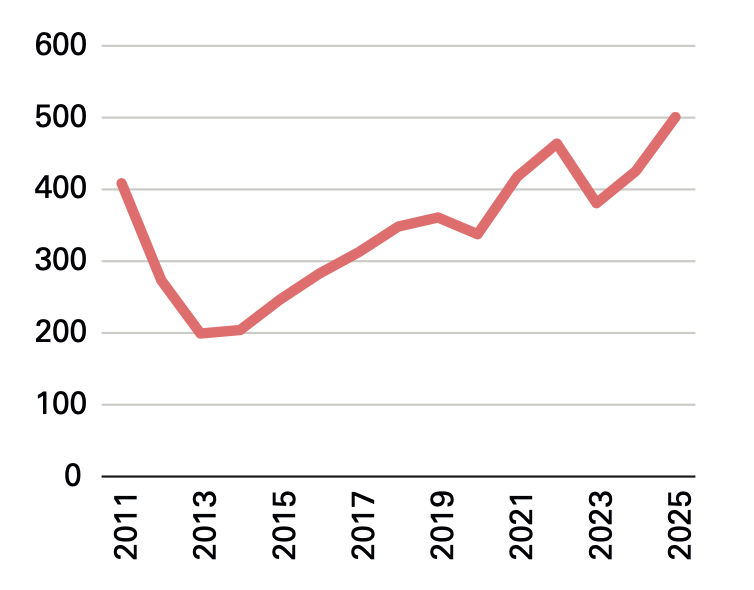
\includegraphics[width=0.6\linewidth]{hipotecas-en-miles.png}}
\end{figure}

\paragraph*{Series temporales multivariables}\mbox{}

Existen problemas de series temporales que no se pueden describir únicamente con una variable, sino que es necesario el uso de múltiples variables que \textit{pueden} estar correlacionadas. Este tipo de series temporales se denominan \textit{series temporales multivariadas}, denotadas por el vector $\{\mathbf{X}_t\}$, en la que no solo existe dependencia dentro de cada componente $\{X_{ti}\}$, sino también interdependencia entre distintos componentes de la serie, $\{X_{ti}\}$ y $\{X_{tj}\}$, con $i \neq j$. Gran parte de la teoría de series temporales univariantes se extiende casi de forma natural al caso multivariante \cite{Brockwell2006}. Expandiendo las componentes podemos escribir la serie como:
$$
    \mathbf{X}_t =
    \begin{pmatrix}
        X_{t1} \\
        X_{t2} \\
        \vdots \\
        X_{tp}
    \end{pmatrix},
    \qquad t \in \mathcal{T}
$$

donde cada componente $X_{ti}$ representa la variable aleatoria $i$-ésima observada en el instante $t$, para $i = 1, 2, \ldots, p$.

\begin{figure}[H]
    \ffigbox[\FBwidth] {
        \caption[Ejemplo de serie temporal multivariante]{Ejemplo de serie temporal multivariante: tasa de cambio de los pares EUR/USD y GBP/USD del 01/01/2024 al 01/01/2026 \cite{tradingview_eurusd_gbpusd_2026}.}
    }
    {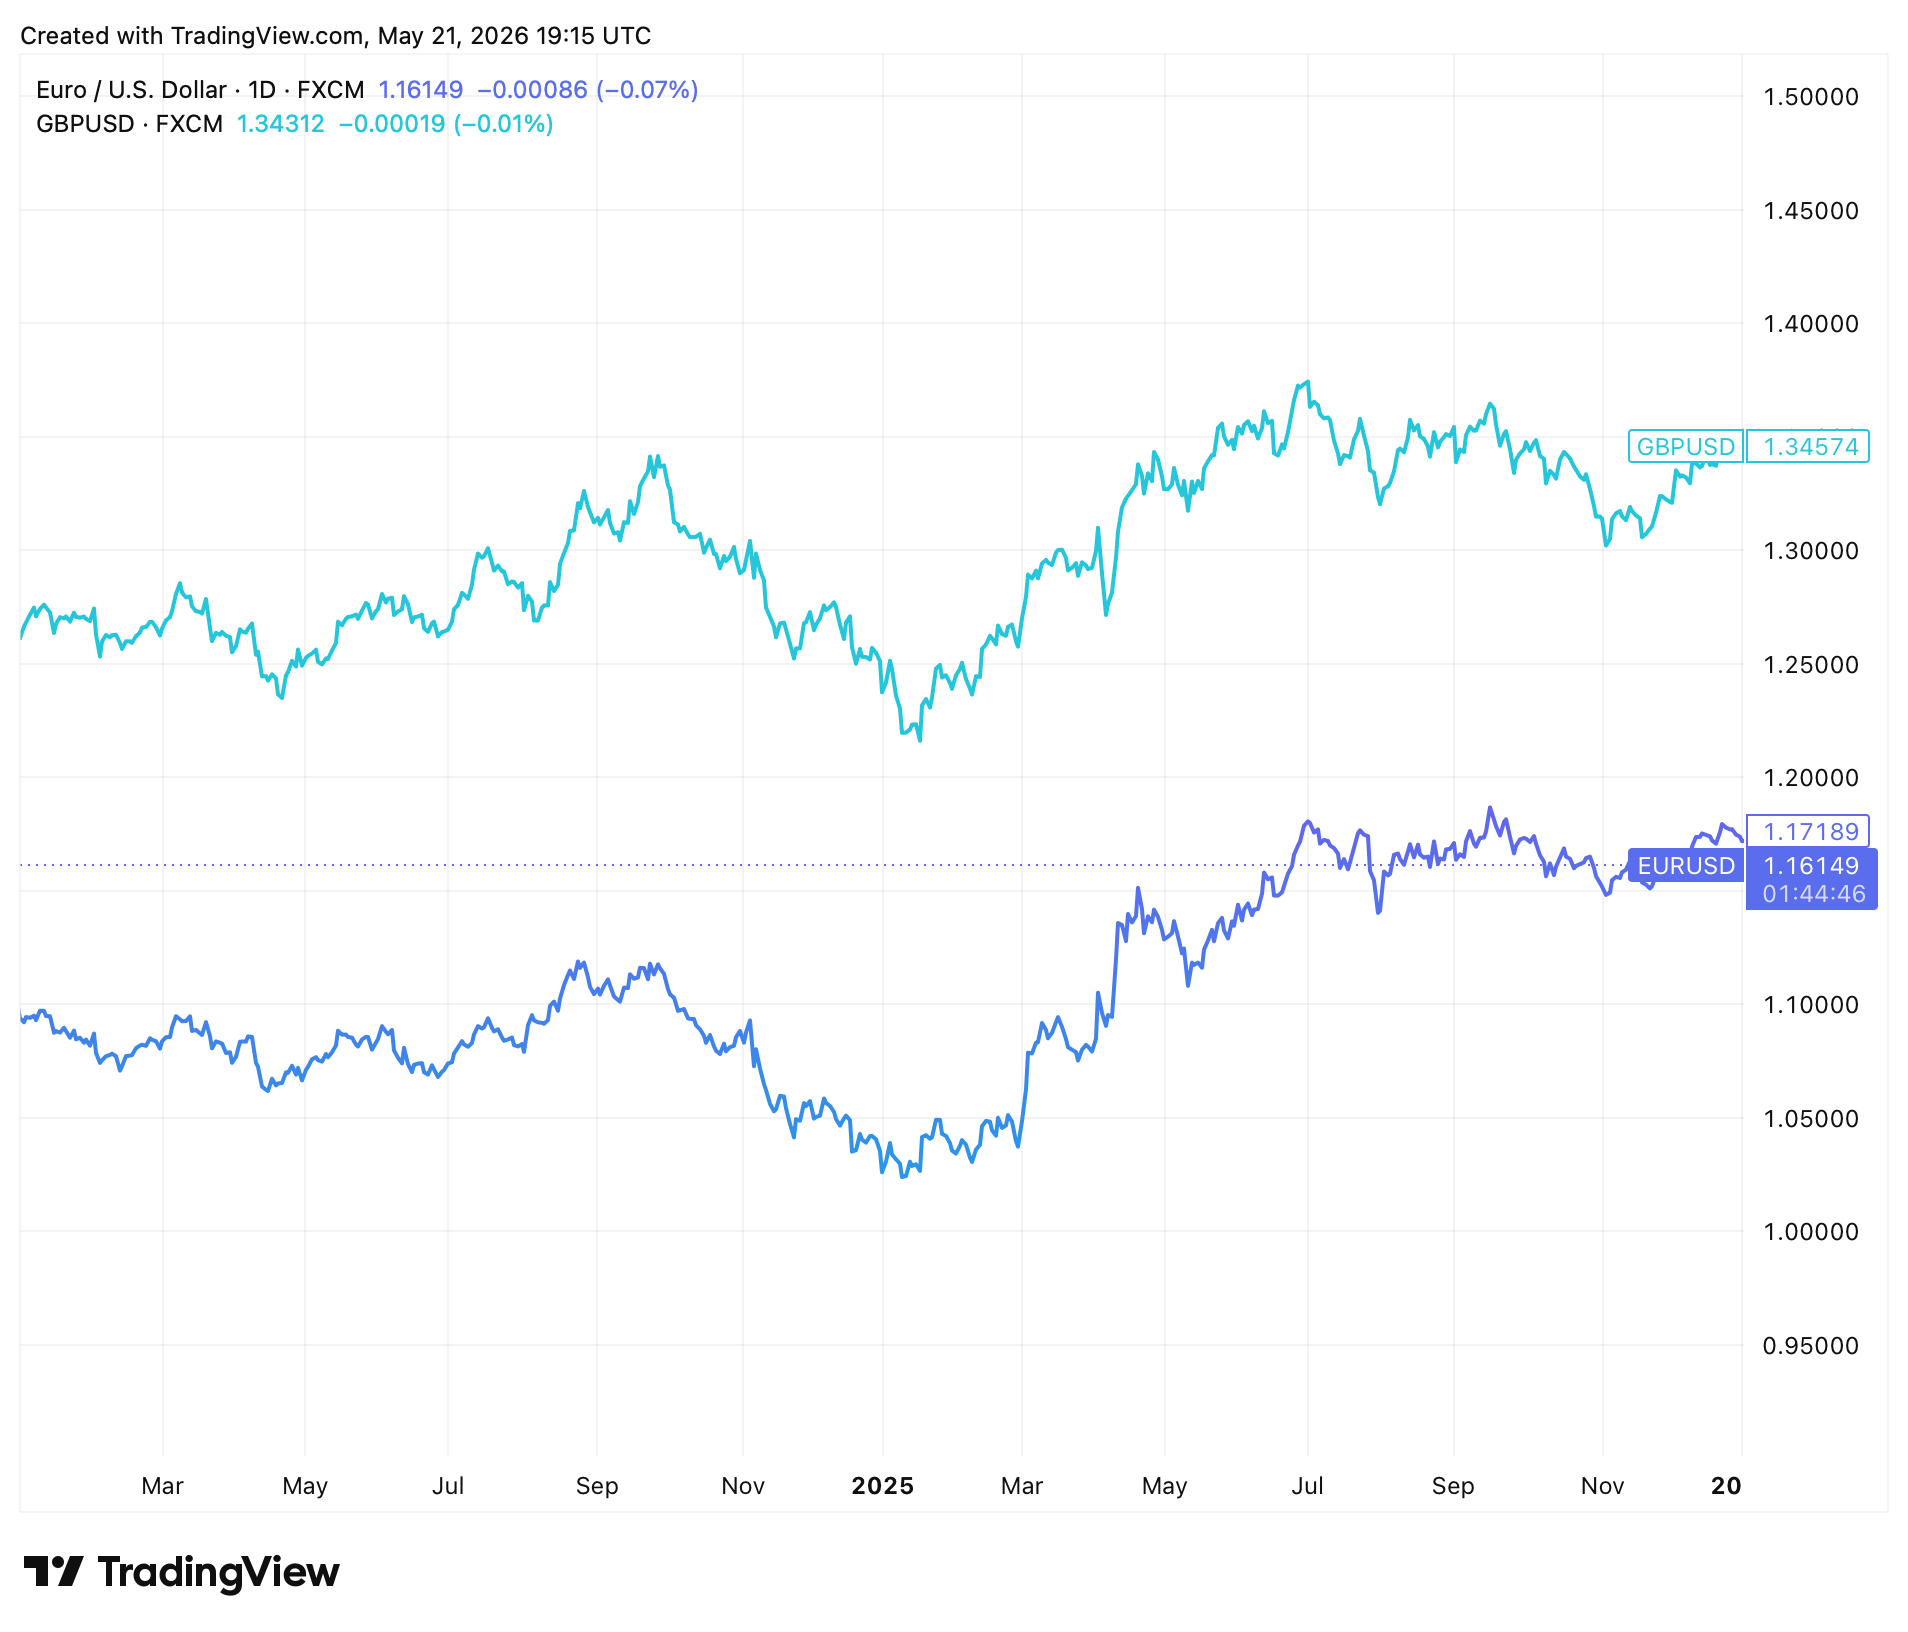
\includegraphics[width=0.8\linewidth]{EURUSD_2026-05-21_21-15-14.png}}
\end{figure}

\subsection{Taxonomía de problemas en series temporales}

Las series temporales como dato pueden ser de interés desde múltiples perspectivas: predecir la evolución de la serie, comparar varias series, decidir si un punto en una serie es una anomalía, etc. Esta taxonomía se recoge de \cite{Fu2011}, \cite{Esling2012}, \cite{Ding2008} y \cite{Anderson1994}.

Para todos y cada unos de los siguientes tipos de problemas, se pueden encontrar formulación en el caso univariante como el multivariante.
\paragraph{Regresión}\mbox{}

La regresión es una tarea supervisada cuyo objetivo consiste en predecir el valor de una variable de interés a partir de una o varias variables explicativas. En el contexto de las series temporales, este planteamiento permite relacionar la evolución en el tiempo para una magnitud objetivo, con información observada en instantes anteriores. Por ejemplo, puede resultar útil explicar las ventas mensuales a partir del gasto publicitario, o anticipar la demanda eléctrica diaria a partir de la temperatura. La variable que se desea pronosticar suele denominarse variable dependiente, respuesta o explicada, mientras que las variables utilizadas para construir la predicción se conocen como regresores o variables explicativas.

Desde el punto de vista estadístico, la regresión en series temporales busca aproximar la dependencia entre la variable objetivo y sus variables explicativas mediante una relación funcional suficientemente simple como para ser interpretable y suficientemente flexible como para proporcionar buenas predicciones \cite{Hyndman2021}. Dependiendo del horizonte considerado, el problema puede plantearse como una predicción de un solo paso o como una predicción de varios pasos hacia delante.

\textbf{Regresión lineal simple.} El caso más elemental aparece cuando se utiliza un único predictor. Entonces la relación entre la variable objetivo $y$ y la variable explicativa $x$ puede escribirse como:
$$
    y_t = \beta_0 + \beta_1 x_t + \varepsilon_t
$$
En esta expresión, $\beta_0$ representa el intercepto y $\beta_1$ la pendiente de la recta de regresión. El primero indica el valor esperado de $y_t$ cuando $x_t = 0$, mientras que el segundo recoge la variación media esperada en $y_t$ ante un aumento unitario de $x_t$. El término $\varepsilon_t$ agrupa la parte no explicada por el modelo; no debe interpretarse como un error en sentido coloquial, sino como la contribución de todos aquellos factores que influyen en la varianza de $y_t$ y que no han quedado incorporados explícitamente en la ecuación, incluyendo el ruido.

\textbf{Regresión lineal múltiple.} Cuando la predicción depende de varias variables explicativas, la especificación anterior se extiende de forma natural a
\begin{equation}
    y_t = \beta_0 + \beta_1 x_{1,t} + \beta_2 x_{2,t} + \cdots + \beta_k x_{k,t} + \varepsilon_t,
    \label{eq:multiple_linear_regression}
\end{equation}
donde $x_{1,t}, \ldots, x_{k,t}$ son variables numéricas observadas en el instante $t$. En este caso, cada coeficiente $\beta_j$ debe interpretarse como el efecto marginal del predictor correspondiente una vez controlado el efecto del resto de variables incluidas en el modelo, es decir manteniendo constantes las demás variables.

\textbf{Supuestos del modelo.} La utilidad de la regresión lineal depende de varios supuestos:
\begin{itemize}
    \item La relación lineal propuesta sea una aproximación razonable del fenómeno estudiado.
    \item Los errores $(\varepsilon_1, \ldots, \varepsilon_T)$ tengan media cero.
    \item Los errores no presenten autocorrelación.
    \item Los errores sean independientes de las variables explicativas.
    \item Los errores sigan una distribución normal con varianza constante $\sigma^2$.
\end{itemize}

Si estas condiciones no se cumplen, las estimaciones pueden resultar sesgadas o ineficientes, y parte de la estructura presente en los datos quedaría sin modelizar. En particular, la hipótesis de normalidad con varianza constante simplifica la construcción de intervalos de predicción, que no deben confundirse con los intervalos de confianza.

Por último, el modelo lineal clásico trata las variables explicativas como variables fijadas externamente. En experimentos controlados esta hipótesis es natural, pero con datos observacionales, como ocurre en muchas aplicaciones económicas y empresariales, los valores de las variables explicativas no se controlan sino que simplemente se observan. En consecuencia, dicho supuesto debe entenderse como una idealización analítica que facilita el estudio del problema, no como una descripción literal del proceso generador de los datos.

\textbf{Predicción con modelos lineales.}

Una vez estimados los coeficientes del modelo (por ejemplo, mediante mínimos cuadrados ordinarios), la predicción puntual de la variable objetivo puede obtenerse sustituyendo las estimaciones y los valores observados de las variables explicativas en la ecuación de regresión. En el caso de un modelo lineal múltiple, la predicción ajustada viene dada por
\begin{equation}
    \hat{y}_t = \hat{\beta}_0 + \hat{\beta}_1 x_{1,t} + \hat{\beta}_2 x_{2,t} + \cdots + \hat{\beta}_k x_{k,t},
    \label{eq:linear_fitted_values}
\end{equation}
donde el término de error no aparece porque la predicción trabaja con el valor esperado condicional de $y_t$. Si esta expresión se evalúa para $t = 1, \ldots, T$ usando los valores observados de las variables explicativas en la muestra, se obtienen los valores ajustados del conjunto de entrenamiento. Sin embargo, en series temporales el interés principal no suele estar en reproducir la muestra histórica, sino en anticipar valores futuros de la variable objetivo \cite{Hyndman2021}.

\textbf{Predicciones \textit{ex ante} y \textit{ex post}.} En regresión para series temporales conviene distinguir entre dos tipos de predicción según la información disponible en el momento de calcularlas. Las predicciones \textit{ex ante} se elaboran utilizando únicamente la información conocida con anterioridad al periodo que se quiere pronosticar; por tanto, constituyen predicciones genuinas. Su principal dificultad es que requieren disponer también de valores futuros para las variables explicativas, lo que obliga a pronosticar esos regresores con modelos adicionales o a recurrir a proyecciones externas. En cambio, las predicciones \textit{ex post} se calculan una vez conocidos los valores efectivamente observados de las variables explicativas. No son pronósticos genuinos, pero resultan útiles para estudiar el comportamiento del modelo y descomponer el origen de los errores de predicción.

La comparación entre predicciones \textit{ex ante} y \textit{ex post} es especialmente útil porque permite separar dos fuentes de incertidumbre: la incertidumbre asociada al propio modelo de regresión y la derivada de tener que pronosticar las variables explicativas.

Un ejemplo de esta diferencia se encuentra en los modelos que predicen precipitaciones. Una predicción \textit{ex ante} nos permite predecir la lluvia del siguiente periodo. Una predicción \textit{ex post} nos permite, usando valores históricos, comparar la predicción con la cantidad real de lluvia, para poder dar una estimación de cuánto se desvía la lluvia actual respecto a lo esperado; es una de las formas de medir los efectos del cambio climático.

\textbf{Modelos predictivos con retardos.} Una forma habitual de hacer la regresión consiste en emplear como regresores valores retardados de las variables explicativas. Si el objetivo es obtener una predicción a $h$ pasos, una formulación natural es
\begin{equation}
    y_{t+h} = \beta_0 + \beta_1 x_{1,t} + \cdots + \beta_k x_{k,t} + \varepsilon_{t+h},
    \qquad h \geq 1
    \label{eq:lagged_predictive_regression}
\end{equation}
En esta especificación, las variables explicativas se observan $h$ periodos antes que la variable que se desea pronosticar. Esto tiene una ventaja práctica importante: al proyectar el modelo más allá del final de la muestra, los valores de entrada ya son conocidos y no es necesario predecir simultáneamente todas las variables explicativas. Además, esta formulación suele ser más verosímil ya que muchos efectos no se materializan de forma instantánea, sino con cierto retraso \cite{Anderson1994}. Cuando incluso esta estrategia resulta insuficiente, puede recurrirse a análisis por escenarios, fijando trayectorias plausibles para las variables explicativas y evaluando cómo cambian las predicciones del modelo bajo cada una de ellas.

\textbf{Intervalos de predicción.} Junto a la predicción puntual, en la práctica interesa cuantificar su incertidumbre. En el caso de la regresión lineal simple, y bajo el supuesto de errores normales, un intervalo de predicción aproximado al $95\%$ para una nueva observación puede expresarse como
\begin{equation}
    \hat{y} \pm 1.96\,\hat{\sigma}_e\sqrt{1 + \frac{1}{T} + \frac{(x - \bar{x})^2}{(T-1)s_x^2}}
    \label{eq:simple_regression_prediction_interval}
\end{equation}
donde $T$ es el tamaño muestral, $\bar{x}$ es la media observada del predictor, $s_x$ es su desviación típica y $\hat{\sigma}_e$ es el error estándar residual. Para niveles de cobertura distintos basta con reemplazar el valor $1.96$ por el cuantil correspondiente. Esta expresión muestra además que la incertidumbre de la predicción crece cuando el valor del predictor se aleja de su media muestral, lo que refleja que el modelo predice con mayor precisión en regiones del espacio de entrada bien representadas por los datos observados \cite{Hyndman2021}.

\textbf{Forma matricial.} En problemas con múltiples observaciones y varias variables explicativas, resulta conveniente escribir el modelo en forma matricial. Sea
$$
    \mathbf{y} = (y_1, \ldots, y_T)^\top
    \qquad
    \boldsymbol{\varepsilon} = (\varepsilon_1, \ldots, \varepsilon_T)^\top
    \qquad
    \boldsymbol{\beta} = (\beta_0, \beta_1, \ldots, \beta_k)^\top
$$
y sea además la matriz de datos $X$ de dimensión $T \times (k+1)$, donde la primera columna es un vector de unos para el intercepto y las siguientes columnas contienen los valores de las variables explicativas para cada observación:
$$
    X =
    \begin{pmatrix}
        1      & x_{1,1} & x_{2,1} & \cdots & x_{k,1} \\
        1      & x_{1,2} & x_{2,2} & \cdots & x_{k,2} \\
        \vdots & \vdots  & \vdots  & \ddots & \vdots  \\
        1      & x_{1,T} & x_{2,T} & \cdots & x_{k,T}
    \end{pmatrix}
$$
Con esta notación, el modelo de regresión lineal puede escribirse de forma compacta como
\begin{equation}
    \mathbf{y} = X\boldsymbol{\beta} + \boldsymbol{\varepsilon}
    \label{eq:matrix_regression_model}
\end{equation}
donde se asume que $\mathbb{E}[\boldsymbol{\varepsilon}] = \mathbf{0}$ y $\operatorname{Var}(\boldsymbol{\varepsilon}) = \sigma^2 I$. La matriz $X$ tiene $T$ filas, una por observación, y $k+1$ columnas, correspondientes al intercepto y a las $k$ variables explicativas incluidas en el modelo.

\textbf{Estimación por mínimos cuadrados.} En esta formulación, la estimación por mínimos cuadrados ordinarios se obtiene minimizando la suma de cuadrados residual,
$$
    \boldsymbol{\varepsilon}^\top \boldsymbol{\varepsilon}
    =
    (\mathbf{y} - X\boldsymbol{\beta})^\top (\mathbf{y} - X\boldsymbol{\beta}).
$$
La solución del problema viene dada por la ecuación:
\begin{equation}
    \hat{\boldsymbol{\beta}} = (X^\top X)^{-1} X^\top \mathbf{y}.
    \label{eq:normal_equation}
\end{equation}
Esta expresión requiere que $X$ tenga rango columna completo (por el Teorema de Rouché-Frobenius); de lo contrario, si la matriz $X^\top X$ es singular (no invertible) entonces el modelo no puede estimarse de forma única. Este problema aparece, por ejemplo, cuando se incluyen variables indicadoras redundantes y se incurre en la denominada \textit{dummy variable trap}. La varianza residual puede estimarse mediante
\begin{equation}
    \hat{\sigma}_e^2 = \frac{1}{T-k-1}(\mathbf{y} - X\hat{\boldsymbol{\beta}})^\top (\mathbf{y} - X\hat{\boldsymbol{\beta}}).
    \label{eq:residual_variance_matrix}
\end{equation}

\textbf{Valores ajustados y validación cruzada.} La ecuación permite expresar los valores ajustados como
\begin{equation}
    \hat{\mathbf{y}} = X\hat{\boldsymbol{\beta}} = X(X^\top X)^{-1}X^\top \mathbf{y} = H\mathbf{y},
    \label{eq:hat_matrix}
\end{equation}
donde $H = X(X^\top X)^{-1}X^\top$ se conoce como matriz sombrero, ya que transforma $\mathbf{y}$ en $\hat{\mathbf{y}}$. Si se denotan por $h_1, \ldots, h_T$ los elementos diagonales de $H$, el estadístico de validación cruzada de tipo \textit{leave-one-out} puede calcularse como
\begin{equation}
    \operatorname{CV} = \frac{1}{T}\sum_{t=1}^{T}\left(\frac{e_t}{1-h_t}\right)^2,
    \label{eq:cv_hat_matrix}
\end{equation}
donde $e_t$ es el residuo obtenido al ajustar el modelo con las $T$ observaciones. Esta identidad evita tener que reestimar el modelo $T$ veces para evaluar el error de predicción fuera de muestra (\textit{out-of-sample})\cite{Hyndman2021}.

\textbf{Predicción e intervalos en forma matricial.} Sea $\mathbf{x}_*$ un vector fila que contiene los valores de las variables explicativas, con el mismo formato que las filas de $X$, para los que se desea obtener una predicción. Entonces, la predicción puntual viene dada por
\begin{equation}
    \hat{y}_* = \mathbf{x}_*\hat{\boldsymbol{\beta}} = \mathbf{x}_*(X^\top X)^{-1}X^\top \mathbf{y}
    \label{eq:forecast_matrix_form}
\end{equation}
y la varianza estimada de predicción puede escribirse como
\begin{equation}
    \hat{\sigma}_e^2\left[1 + \mathbf{x}_*(X^\top X)^{-1}\mathbf{x}_*^\top\right]
    \label{eq:forecast_variance_matrix}
\end{equation}
Bajo el supuesto de errores normales, un intervalo de predicción aproximado al $95\%$ adopta la forma
\begin{equation}
    \hat{y}_* \pm 1.96\,\hat{\sigma}_e\sqrt{1 + \mathbf{x}_*(X^\top X)^{-1}\mathbf{x}_*^\top}
    \label{eq:forecast_prediction_interval_matrix}
\end{equation}
Este intervalo incorpora tanto la incertidumbre asociada al término de error como la incertidumbre causada por estimar los coeficientes del modelo. Sin embargo, no recoge la incertidumbre adicional procedente de posibles errores en los valores futuros de las variables explicativas.

\textbf{Correlación, causalidad y predicción.} En modelos predictivos (tanto si son de series temporales como si no lo son) es necesario distinguir entre correlación, causalidad y poder de predicción. Que una variable $x$ resulte útil para predecir otra variable $y$ no implica, por sí mismo, que $x$ cause a $y$. La relación observada puede deberse a una causalidad en sentido contrario ($y$ causa a $x$) o a la presencia de una tercera variable omitida que influya simultáneamente sobre ambas; un factor de confusión. Un ejemplo clásico es la asociación entre las ventas de helados y el número de ahogamientos en una zona costera \cite{pearl2017}: ambas variables pueden moverse juntas sin que exista una relación causal directa entre ellas, simplemente porque las dos aumentan cuando sube la temperatura. En este caso, la temperatura actúa como variable de confusión, es decir, como una variable no incluida en el modelo que influye tanto sobre la respuesta como sobre al menos una de las variables explicativas.

Tampoco debe identificarse causalidad con dirección de predicción. Es posible construir un modelo predictivo razonable incluso cuando la relación causal relevante apunta en sentido opuesto al modelo de predicción. Por ejemplo, un descenso inusual en el número de ciclistas por la mañana puede anticipar lluvia por la tarde, no porque los ciclistas modifiquen el tiempo atmosférico, sino porque la previsión meteorológica influye previamente sobre la decisión de desplazarse en bicicleta. En consecuencia, las correlaciones pueden ser valiosas para predecir aun cuando no exista un vínculo causal directo, cuando la causalidad sea inversa o cuando intervengan factores de confusión.

\textbf{Predictores correlacionados.} Cuando dos o más variables explicativas están muy correlacionadas, resulta difícil separar con precisión sus efectos individuales. Esta situación no impide necesariamente obtener buenas predicciones, porque el modelo puede seguir explotando la información conjunta contenida en esas variables, pero sí complica tareas como la predicción por escenarios o el análisis de la contribución de cada variable (análisis de sensibilidades), ya que cualquier cambio hipotético en una variable debería ser coherente con su relación histórica con las demás.

\textbf{Multicolinealidad.} Un caso especialmente relevante de esta dificultad es la multicolinealidad, que aparece cuando dos o más variables explicativas aportan información muy similar dentro de un modelo de regresión múltiple. Puede manifestarse porque dos variables estén altamente correlacionadas entre sí, o porque una combinación lineal de algunas variables esté casi perfectamente relacionada con otra combinación lineal distinta. El ejemplo más conocido es la \textit{dummy variable trap}: si se incluyen variables indicadoras para todas las categorías de una variable cualitativa junto con un intercepto, una de ellas queda determinada exactamente por las demás y aparece una dependencia lineal perfecta.

\paragraph*{Clusterización}\mbox{}

La tarea de clusterización trata de encontrar agrupaciones (\textit{clusters}) de series temporales similares entre sí. Este tipo de problemas se considera de información completa y son problemas no supervisados, ya se basa en usar una función de homogeneidad que agrupe series lo más similares entre sí y lo más distintas entre grupos. Un ejemplo típico en finanzas es clusterizar los movimientos de pares de monedas, y descubrir si ciertos pares de monedas se mueven respecto a una moneda "base", para conocer si se agrupan entorno a los movimiento del dólar, el euro o el yen.

\paragraph*{Similaridad}\mbox{}

La tarea de similaridad consiste en cuantificar hasta qué punto dos series temporales se asemejan, mediante una función de distancia $\operatorname{Dist}(T, T')$. Se trata de un problema no supervisado, ya que no depende de etiquetas, sino de cómo se define la proximidad entre secuencias posiblemente ruidosas, desalineadas en el tiempo o incluso muestreadas a ritmos distintos \cite{Ding2008,Fu2011}. Una clasificación habitual distingue entre medidas de tipo \textit{lock-step}, que comparan el punto $i$-ésimo de una serie con el punto $i$-ésimo de la otra, y medidas elásticas, que permiten tanto correspondencias de uno a muchos como deformaciones temporales \cite{Ding2008}.

Dentro del primer grupo destacan las distancias inducidas por normas $L_p$, y en particular la distancia euclídea $L_2$, por su simplicidad, coste lineal y facilidad de indexación, aunque son sensibles al ruido y a los desfases locales \cite{Faloutsos1994}. Entre las medidas elásticas, \textit{dynamic time warping} (DTW) permite comprimir o estirar localmente una serie para mejorar el emparejamiento \cite{BerndtClifford1994}, mientras que la familia de distancias basadas en edición, como LCSS, EDR y ERP, tolera huecos, emparejamientos parciales y discrepancias locales \cite{Ding2008,ChenOzsuOria2005,ChenNg2004}.

Si $T = (x_1, \ldots, x_n)$ y $T' = (x'_1, \ldots, x'_n)$ son dos series de igual longitud, una familia clásica de medidas \textit{lock-step} viene dada por las distancias inducidas por normas $L_p$:
$$
    d_p(T, T') = \left(\sum_{i=1}^{n} |x_i - x'_i|^p\right)^{1/p}, \qquad p \geq 1.
$$
Como casos particulares se obtienen la distancia Manhattan, $d_1$, la distancia euclídea, $d_2$, y la distancia máxima,
$$
    d_{\infty}(T, T') = \max_{1 \leq i \leq n} |x_i - x'_i|.
$$
Estas medidas son atractivas por su simplicidad, coste lineal y facilidad de indexación, aunque resultan sensibles al ruido y a los desfases locales \cite{Faloutsos1994}.

Entre las medidas elásticas, DTW (\textit{Dynamic Time Warping}) permite comprimir o estirar localmente una serie para mejorar el emparejamiento \cite{BerndtClifford1994}. Si $T = (x_1, \ldots, x_n)$ y $T' = (x'_1, \ldots, x'_m)$, con $n \neq m$, la distancia se expresa como:
$$
    \operatorname{DTW}(T, T') = D(n,m),
$$
$$
    D(0,0)=0, \qquad D(i,0)=D(0,j)=+\infty,
$$
$$
    D(i,j) = |x_i - x'_j| + \min\{D(i-1,j), D(i,j-1), D(i-1,j-1)\},
$$
para $1 \leq i \leq n$ y $1 \leq j \leq m$. Por su parte, una forma normalizada de la medida LCSS (\textit{Longest Common Subsequence}) puede escribirse como
$$
    d_{\mathrm{LCSS}}(T, T') = 1 - \frac{\mathrm{LCSS}_{\varepsilon,\delta}(T, T')}{\min(n,m)},
$$
donde $\varepsilon$ controla la tolerancia en amplitud y $\delta$ la tolerancia temporal. Esta familia de distancias basadas en edición, junto con EDR (\textit{Edit Distance on Real sequence}) y ERP (\textit{Edit Distance with Real Penalty}), tolera huecos, emparejamientos parciales y discrepancias locales \cite{Ding2008,ChenOzsuOria2005,ChenNg2004,Morse2007}.

Existen además propuestas más especializadas, como TQuEST (\textit{Threshold Query based Similarity Search}), basada en intervalos de cruce de umbral, o SpADe (\textit{Shape-based Pattern Detection}), orientada a detectar patrones con desplazamientos y escalados en tiempo y amplitud \cite{Assfalg2006,Chen2007SpADe}. En la práctica, la elección de la medida de similaridad depende del equilibrio deseado entre robustez frente a desalineaciones, número de parámetros, interpretabilidad y coste computacional \cite{Ding2008}.

\paragraph{Clasificación}\mbox{}

La clasificación de series temporales trata de asignar una etiqueta (\textit{label}) a la serie. Este tipo de problemas se considera de información completa, ya que se dispone de la serie completa para tomar la decisión. Por ejemplo, clasificar una serie temporal de temperatura como \textit{cómoda} o \textit{incómoda}. Entra dentro de la clase de problemas supervisados, ya que se dispone de un conjunto de entrenamiento con series temporales etiquetadas.

Dentro de la tarea de clasificación se pueden distinguir dos subtipos de problemas:
\begin{itemize}
    \item Clasificación de series temporales completas, donde se asigna una etiqueta a toda la serie.
    \item Clasificación de instantes temporales, donde se asigna una etiqueta a un único instante temporal de la serie. Dentro de subtipo se encuentra la tarea de detección de anomalías, donde se asigna una etiqueta de \textit{normal} o \textit{anómalo} a cada instante temporal de la serie.
\end{itemize}

Las técnicas principales para clasificar series temporales se pueden diferenciar entre \cite{faouzi:hal-03558165}:
\begin{itemize}
    \item Basadas en métricas: \textit{knn} con distancia DTW
    \item Basadas en kernel: \textit{SVM}.
    \item Basados en deep learning: modelos de redes de neuronas, en cualquiera de sus arquitecturas.
\end{itemize}

\paragraph*{Segmentación}\mbox{}

También conocido como resumen, tiene por objetivo crear una nueva serie temporal, derivada de la original, usando la menor cantidad de datos posibles y conservando la mayor cantidad de información posible. Se considera un subproblema del problema de la discretización, dado que se busca reducir la cantidad de datos a través de la creación de segmentos o resúmenes de la serie temporal original.

\section{Causalidad \textit{Pearliana}}

El estudio de la causalidad permite interpretar los datos (observaciones) más allá de simples relaciones entre variables, dado un modelo causal.
También ayuda a estimar efectos concretos, como el impacto del tabaco, políticas públicas, etc.
A diferencia de la estadística clásica, la causalidad \textit{añade} un marco conceptual capaz de describir relaciones de causa y efecto que el lenguaje estadístico estándar no puede expresar por sí solo. El lenguaje causal descrito por \textit{Pearl} amplía las respuestas allí donde las herramientas estadísticas tradicionales no son capaces de llegar.

Una de las mejores metáforas sobre la relación de las causas y efectos, y nuestro conocimiento sobre estos, se encuentra en el libro divulgativo \textit{The book of why} del propio Judea Pearl. En él se explica la \textit{La escalera de la causalidad}, una metáfora en la que se según se sube la escalera, más seguros podemos encontrarnos de que las causas y efectos son reales, siendo los peldaños la \textbf{asociación}, la \textbf{intervención} y los \textbf{contrafactuales}; cada peldaño requiere herramientas matemáticas distintas y responde a preguntas diferentes \cite{pearl2017}.

Para motivar el estudio de la causalidad Pearliana se suele usar la paradoja de Simpson, popularizada por Edward Simpson: a un grupo de pacientes enfermos se les ofrece la posibilidad de probar un nuevo fármaco. Entre quienes toman el medicamento, el porcentaje de recuperación es \textit{menor} que entre quienes no lo toman. Sin embargo, al desagregar los datos por sexo, se observa que se recuperan más hombres que toman el fármaco que hombres que no lo toman, y también se recuperan más mujeres que toman el fármaco que mujeres que no lo toman. En otras palabras, el medicamento parece beneficiar tanto a hombres como a mujeres, pero \textit{perjudicar a toda población} considerada en conjunto \cite{Simpson1951}. El resultado parece absurdo, o incluso imposible, y precisamente por eso se considera una paradoja.

Un ejemplo con datos continuos más relacionado con el campo de la informática: a los usuarios que se les muestra más un anuncio publicitario, se les observa una menor tasa de conversión (por ejemplo, comprar un producto). Sin embargo, al desagregar por edad, se observa que en cada grupo de edad, los usuarios que ven más el anuncio tienen una mayor tasa de conversión. En este caso, la variable de confusión es la edad: los usuarios más jóvenes son más propensos a comprar el producto, independientemente de la cantidad de publicidad; existe un sesgo de variable omitida, que ha provocado que el coeficiente de la regresión tenga signo contrario.

\begin{figure}[H]
    \centering
    \begin{minipage}[t]{0.44\textwidth}
        \centering
        
\includegraphics[width=\linewidth]{conversion_publicidad_1.png}
    \end{minipage}
    \hfill
    \begin{minipage}[t]{0.51\textwidth}
        \centering
        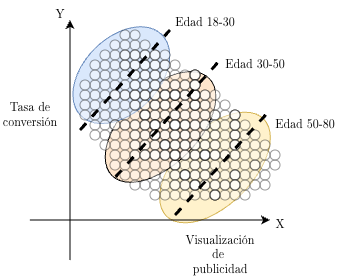
\includegraphics[width=\linewidth]{conversion_publicidad_2.png}
    \end{minipage}
    \caption{Ejemplo de la paradoja de Simpson. Elaboración propia.}
    \label{fig:simpson_paradox_conversion}
\end{figure}

\subsection{Grafos causales como lenguaje matemático}

La paradoja de Simpson muestra que, en problemas causales, los datos observados no siempre bastan para tomar decisiones correctas: es necesario incorporar hipótesis sobre el proceso generador de los datos (DPG, \textit{Data Generating Process}). Ese proceso puede expresarse de forma compacta mediante grafos causales dirigidos acíclicos (DAG, \textit{Directed Acyclic Graphs}) \cite{Pearl2016-nx}.

Un grafo $G=(V,E)$ está formado por un conjunto de nodos $V$ (variables) y un conjunto de aristas $E$ (relaciones). En causalidad, las aristas son dirigidas y se interpretan como influencias causales directas. Si existe una flecha $X \to Y$, entonces $X$ es \textit{padre} de $Y$ y $Y$ es \textit{hijo} de $X$.

Un \textbf{camino} es una secuencia de nodos conectados por aristas. Un \textbf{camino dirigido} sigue la orientación de las flechas. Si existe un camino dirigido de $X$ a $Y$, decimos que $X$ es ancestro de $Y$ y $Y$ descendiente de $X$. Cuando no hay caminos dirigidos que vuelvan al nodo de origen, el grafo es acíclico.

Este lenguaje permite distinguir:
\begin{itemize}
    \item relaciones causales directas (flechas presentes),
    \item asociaciones espurias por confusión (caminos de retroceso o \textit{backdoor}),
    \item y conjuntos de ajuste para estimar efectos causales.
\end{itemize}

En el ejemplo de conversión, se consideran tres variables:
\begin{itemize}
    \item $A$: edad del usuario,
    \item $P$: exposición publicitaria,
    \item $C$: conversión (p.ej., compra).
\end{itemize}

La historia causal compatible con la paradoja de Simpson es:
\begin{itemize}
    \item la edad influye en la exposición ($A \to P$), ya que los más jóvenes no necesitan tanta publicidad para comprar el producto, y viceversa.
    \item la edad influye en la conversión ($A \to C$), ya que los más jóvenes son más propensos a comprar el producto, y viceversa.
    \item y la exposición puede influir causalmente en la conversión ($P \to C$).
\end{itemize}

El DAG correspondiente es:

\begin{figure}[H]
    \centering
    \begingroup
    \shorthandoff{<>}
    \begin{tikzpicture}[node distance=3.1cm]
        \node (UA) [draw, circle, dashed, minimum size=10mm] at (0, 1.9) {$U_A$};
        \node (UP) [draw, circle, dashed, minimum size=10mm] at (3.1, 1.9) {$U_P$};
        \node (UC) [draw, circle, dashed, minimum size=10mm] at (6.2, 1.9) {$U_C$};
        \node (A) [draw, circle, minimum size=10mm] {$A$};
        \node (P) [draw, circle, right=of A, minimum size=10mm] {$P$};
        \node (C) [draw, circle, right=of P, minimum size=10mm] {$C$};

        \draw[-{Latex}, thick, dashed] (UA) -- (A);
        \draw[-{Latex}, thick, dashed] (UP) -- (P);
        \draw[-{Latex}, thick, dashed] (UC) -- (C);
        \draw[-{Latex}, thick] (A) -- (P);
        \draw[-{Latex}, thick, bend left=22] (A) to (C);
        \draw[-{Latex}, thick] (P) -- (C);
    \end{tikzpicture}
    \endgroup
    \caption[DAG de conversión publicitaria]{DAG para el ejemplo de conversión publicitaria. $U_A$, $U_P$ y $U_C$ representan factores exógenos no observados; $A$: edad, $P$: exposición publicitaria, $C$: conversión.}
    \label{fig:dag_conversion_publicidad}
\end{figure}

Este grafo hace explícito un \textit{factor de confusión} entre $P$ y $C$:
$$
P \leftarrow A \rightarrow C
$$

\subsection{Modelos causales estructurales}

Un \textbf{modelo causal estructural} (MCE, o SCM \textit{Structural Causal Model}) describe cómo un modelo causal asigna valores a las variables de interés. Consta de dos conjuntos de variables $U$ y $V$, y un conjunto de funciones $\mathbf{f}$:
\begin{itemize}
    \item Las variables de $U$ son \textbf{exógenas}: externas al modelo, sin ancestros, representadas como nodos raíz en el grafo.
    \item Las variables de $V$ son \textbf{endógenas}: cada una recibe su valor de una función $f_i \in \mathbf{f}$ que depende de otras variables del modelo.
\end{itemize}

Una variable $X$ es \textbf{causa directa} de $Y$ si $X$ aparece en $f_Y$; es \textbf{causa} de $Y$ si lo es de forma directa o a través de otras causas. El grafo asociado al MCE contiene un nodo por variable y una arista dirigida $Y \to X$ siempre que $Y$ aparezca en $f_X$; trabajaremos con MCE cuyo grafo sea un DAG.

El modelo gráfico resulta útil porque, aunque contiene menos información que el MCE completo (no especifica la forma funcional de cada $f_i$), permite razonar sobre la estructura causal de forma intuitiva con solo inspeccionar las aristas.

En el ejemplo de conversión, el MCE es:
\begin{equation}
    \begin{cases}
        A := U_A \\
        P := f_P(A,\,U_P) \\
        C := f_C(P,\,A,\,U_C)
    \end{cases}
    \label{eq:scm_conversion}
\end{equation}
donde $U_A$, $U_P$ y $U_C$ son factores exógenos no observados (características demográficas no capturadas, ruido en la asignación publicitaria e influencias externas sobre la compra). La edad $A$ es exógena: no puede ser causada por $P$ ni por $C$. El grafo asociado coincide con el DAG de la Figura~\ref{fig:dag_conversion_publicidad}.

Gracias al MCE, la pregunta causal queda bien definida: intervenir $do(P=p)$ elimina $f_P$ y fija $P$ exógenamente, bloqueando el camino de confusión $P \leftarrow A \rightarrow C$.

\textbf{Criterio de ajuste por \textit{backdoor}.} Un conjunto de variables $\mathbf{Z}$ satisface el criterio \textit{backdoor} respecto del par $(P, C)$ en un DAG $G$ si:
\begin{enumerate}
    \item Ninguna variable de $\mathbf{Z}$ es descendiente de $P$, y
    \item $\mathbf{Z}$ bloquea todos los caminos de retroceso entre $P$ y $C$, es decir, todos los caminos que comienzan con una arista dirigida hacia $P$.
\end{enumerate}
Cuando $\mathbf{Z}$ satisface el criterio \textit{backdoor}, el efecto causal de $P$ sobre $C$ es identificable a partir de datos observacionales mediante la fórmula de ajuste:
\begin{equation}
    \mathbb{P}(C \mid do(P=p))
    = \sum_{a} \mathbb{P}(C \mid P=p,\, A=a)\,\mathbb{P}(A=a), a \in \{"18-30", "30-50", "50-80"\}
    \label{eq:backdoor_scm_conversion}
\end{equation}
En el ejemplo, $\mathbf{Z} = \{A\}$ satisface ambas condiciones: la edad no es descendiente de la exposición publicitaria, y bloquea el único camino de retroceso $P \leftarrow A \rightarrow C$. La fórmula promedia la relación exposición-conversión dentro de cada estrato de edad usando la distribución marginal de $A$, recuperando así el efecto causal neto de $P$ sobre $C$ y evitando la inversión de signo característica de la paradoja de Simpson.

\subsection{Intervenciones}

El objetivo último de muchos estudios estadísticos es predecir los efectos de las intervenciones. De hecho muchas \textit{respuestas} que dan las herramientas estadísticas no responden a la pregunta correcta; continuando con nuestro ejemplo de la conversión, el técnico de marketing no está interesado en conocer el efecto promedio, sino en el efecto de intervenir sobre la exposición publicitaria. No es lo mismo preguntar \textit{¿qué ocurre con la variable Y si cambia X?} que la pregunta \textit{¿qué ocurre con la variable Y si fijo X a un valor que yo decido?}. Cuando se recogen datos sobre factores asociados a la conversión, se busca en realidad algo sobre lo que intervenir para aumentar su frecuencia. Cuando se realiza un estudio sobre un nuevo fármaco contra el cáncer, se trata de identificar cómo responde la enfermedad de un paciente cuando se interviene medicándolo.

Una mera asociación entre dos variables no significa necesariamente que una de ellas cause a la otra. Esta es una de las razones por las que un experimento controlado aleatorizado (\textit{Randomized Controlled Trial}, RCT) se considera el mejor procedimiento para la investigación causal: en un experimento correctamente aleatorizado, todos los factores que influyen en la variable de resultado o bien son estáticos o bien varían aleatoriamente, excepto uno, de modo que cualquier cambio en la variable de resultado debe atribuirse a ese único factor de entrada.

Desafortunadamente, muchas preguntas de interés no se prestan a experimentos controlados aleatorizados; no es posible encerrar a los usuarios de la web en una sala y asignarles aleatoriamente una cantidad de publicidad.

En los casos en que los experimentos controlados aleatorizados no son factibles, se pueden realizar estudios observacionales, en los que simplemente registran los datos sin controlarlos. El problema de este tipo de estudios es que resulta difícil separar lo causal de lo meramente correlacional. Por eso es necesario contar con un modelo causal previo a la toma de datos.

\textbf{Intervención frente a condicionamiento.} La diferencia entre intervenir sobre una variable y condicionar sobre ella es fundamental. Cuando se interviene sobre una variable en un modelo, se fija su valor: se modifica el sistema y los valores de otras variables cambian como consecuencia. Cuando se condiciona sobre una variable, no se modifica nada; simplemente se restringe la atención al subconjunto de casos en que la variable toma el valor de interés. Lo que cambia en este caso es nuestra percepción del mundo, no el mundo en sí mismo.

Formalmente, esta distinción se refleja en la notación $do$, creada por Pearl. Se distingue entre el caso en que una variable $X$ toma el valor $x$ de forma natural y el caso en que se fija $X = x$ mediante una intervención, denotando este último como $do(X = x)$. Así, $\mathbb{P}(Y = y \mid X = x)$ es la probabilidad de que $Y = y$ condicionada a observar $X = x$, mientras que $\mathbb{P}(Y \mid do(X = x))$ es la probabilidad de $Y = y$ cuando se interviene para hacer $X = x$. En terminología distribucional, $\mathbb{P}(Y = y \mid X = x)$ refleja la distribución poblacional de $Y$ entre los individuos cuyo valor de $X$ es $x$, mientras que $\mathbb{P}(Y = y \mid do(X = x))$ representa la distribución poblacional de $Y$ si el valor de $X$ se fijara en $x$ para \textbf{todos y cada uno} de los individuos de la población. No estamos hablando de un subconjunto de la población, sino de la población completa bajo una intervención.

\textbf{Cirugía sobre el grafo.} Cuando se interviene sobre una variable, se anula su tendencia natural a variar en respuesta a otras variables del sistema. Esto equivale a realizar una \textit{cirugía} sobre el grafo causal: se eliminan todas las aristas dirigidas hacia esa variable. En el ejemplo de conversión, intervenir sobre $P$ para fijarlo en un valor específico implica eliminar la flecha $A \to P$, lo que bloquea el factor de confusión $P \leftarrow A \rightarrow C$ y permite estimar el efecto causal neto de $P$ sobre $C$.

La Figura~\ref{fig:dag_conversion_publicidad_intervenido} muestra esta cirugía sobre el ejemplo anterior. Tras la intervención $do(P=p)$, la exposición publicitaria deja de venir determinada por sus causas habituales y pasa a quedar fijada externamente. Ni $A$ ni $U_P$ influyen ahora sobre $P$.

\begin{figure}[H]
    \centering
    \begingroup
    \shorthandoff{<>}
    \begin{tikzpicture}[node distance=3.1cm]
        \node (UA) [draw, circle, dashed, minimum size=10mm] at (0, 1.9) {$U_A$};
        \node (UC) [draw, circle, dashed, minimum size=10mm] at (6.2, 1.9) {$U_C$};
        \node (A) [draw, circle, minimum size=10mm] {$A$};
        \node (P) [draw, circle, fill=gray!15, minimum size=12mm] at (3.1, 0) {$p$};
        \node (C) [draw, circle, minimum size=10mm] at (6.2, 0) {$C$};
        \node at (3.1, -0.9) {$do(P=p)$};

        \draw[-{Latex}, thick, dashed] (UA) -- (A);
        \draw[-{Latex}, thick, dashed] (UC) -- (C);
        \draw[-{Latex}, thick, bend left=22] (A) to (C);
        \draw[-{Latex}, thick] (P) -- (C);
    \end{tikzpicture}
    \endgroup
    \caption[DAG intervenido de conversión publicitaria]{Grafo causal intervenido para el ejemplo de conversión publicitaria tras aplicar $do(P=p)$. La intervención elimina las aristas entrantes a $P$ y fija externamente su valor.}
    \label{fig:dag_conversion_publicidad_intervenido}
\end{figure}

Una de las suposiciones implícitas es que la intervención no tiene \textit{efectos secundarios no especificados}, es decir, que asignar el valor $X=x$ para un individuo no altera directamente las variables posteriores de forma distinta a la recogida en el modelo. Gráficamente correspondaría a que fuera del modelo no existen aristas adicionales que conecten $X$ con otras variables posteriores; cuando existen efectos secundarios, deben especificarse explícitamente en el modelo causal.

\subsection{Mediación}

Con frecuencia una variable no afecta a otra de una única forma, sino por varias vías simultáneas. Una parte del efecto puede ser directa, y otra parte puede transmitirse indirectamente a través de una variable intermedia, denominada variable \textbf{mediadora}. Distinguir entre ambos mecanismos es útil porque permite entender no solo si una intervención funciona, sino también \textit{cómo} funciona.

En el ejemplo de conversión publicitaria, la exposición a publicidad $P$ puede influir directamente sobre la conversión $C$, pero también puede hacerlo de forma indirecta a través de una variable mediadora $M$, como el recuerdo de marca. En ese caso, el efecto total de $P$ sobre $C$ se descompone en una vía directa $P \to C$ y una vía indirecta $P \to M \to C$.

\begin{figure}[H]
    \centering
    \begingroup
    \shorthandoff{<>}
    \begin{tikzpicture}[node distance=3.1cm]
        \node (P) [draw, circle, minimum size=10mm] {$P$};
        \node (M) [draw, circle, right=of P, minimum size=10mm] {$M$};
        \node (C) [draw, circle, right=of M, minimum size=10mm] {$C$};

        \draw[-{Latex}, thick] (P) -- (M);
        \draw[-{Latex}, thick] (M) -- (C);
        \draw[-{Latex}, thick, bend left=25] (P) to (C);
    \end{tikzpicture}
    \endgroup
    \caption[DAG de mediación publicitaria]{Ejemplo de mediación en conversión publicitaria. La exposición $P$ puede afectar a la conversión $C$ de forma directa y también indirecta a través de la variable mediadora $M$, que puede interpretarse como recuerdo de marca.}
    \label{fig:dag_mediacion_publicidad}
\end{figure}

En principio, podría parecer que para aislar el efecto directo basta con condicionar sobre la variable mediadora. Siguiendo con el ejemplo, una idea ingenua sería comparar la conversión entre usuarios con distinto nivel de exposición publicitaria pero con el mismo nivel de recuerdo de marca. Sin embargo, este razonamiento deja de ser válido cuando existen variables que confunden la relación entre el mediador y el resultado.

Por ejemplo, supóngase que existe una variable $I$ que representa la intención previa de compra. Los usuarios con mayor afinidad pueden recordar mejor el anuncio y, al mismo tiempo, tener mayor probabilidad de convertir. En ese caso, $I$ actúa como factor de confusión entre $M$ y $C$. Entonces, condicionar sobre $M$ no aísla limpiamente el efecto directo de $P$ sobre $C$, porque puede abrir caminos espurios y mezclar dependencia causal con dependencia inducida por selección.

\begin{figure}[H]
    \centering
    \begingroup
    \shorthandoff{<>}
    \begin{tikzpicture}[node distance=3.1cm]
        \node (I) [draw, circle, minimum size=10mm] at (3.1, 1.9) {$I$};
        \node (P) [draw, circle, minimum size=10mm] {$P$};
        \node (M) [draw, circle, right=of P, minimum size=10mm] {$M$};
        \node (C) [draw, circle, right=of M, minimum size=10mm] {$C$};

        \draw[-{Latex}, thick] (P) -- (M);
        \draw[-{Latex}, thick] (M) -- (C);
        \draw[-{Latex}, thick, bend left=25] (P) to (C);
        \draw[-{Latex}, thick] (I) -- (M);
        \draw[-{Latex}, thick] (I) -- (C);
    \end{tikzpicture}
    \endgroup
    \caption[DAG de mediación con confusión]{Ejemplo de mediación con confusión entre el mediador $M$ y el resultado $C$. La variable $I$ representa intención previa de compra o afinidad con la marca.}
    \label{fig:dag_mediacion_publicidad_confundido}
\end{figure}

La dificultad de la mediación consiste en definir qué significa mantener fija la variable mediadora sin introducir sesgos adicionales. La solución causal consiste en no condicionar sobre el mediador, sino \textbf{intervenir} sobre él \cite{Pearl2016-nx}. Si en lugar de restringirnos a usuarios con un mismo valor de $M$, fijamos teóricamente el valor del mediador mediante $do(M=m)$, entonces desaparecen las aristas entrantes a $M$ y se evita que la dependencia espuria pase a través de ellas, incluso cuando las aristas sean desconocidas.

Esto permite definir el \textbf{efecto directo controlado} (\textit{Controlled Direct Effect}, CDE) de cambiar el valor de $P$ desde $p$ hasta $p'$ manteniendo fijo el mediador en $m$:

\begin{equation}
    \operatorname{CDE}(m)
    = \mathbb{P}(C = c \mid do(P=p), do(M=m))
    - \mathbb{P}(C = c \mid do(P=p'), do(M=m))
    \label{eq:cde_publicidad}
\end{equation}

Esta definición expresa la idea de comparar dos mundos posibles que solo difieren en el nivel de exposición publicitaria, mientras el mediador se mantiene constante por intervención. Su ventaja frente al condicionamiento es que sigue siendo válida incluso cuando la relación entre el mediador y el resultado está confundida, siempre que las probabilidades intervenidas sean identificables a partir de los datos observados.

En general, el efecto directo puede depender del valor fijado para el mediador. En el ejemplo publicitario, podría ocurrir que la publicidad tenga poco efecto directo cuando el recuerdo de marca ya es alto, pero un efecto mayor cuando dicho recuerdo es bajo. Por tanto, para describir completamente el efecto directo controlado conviene estudiar varios valores relevantes de $m$; fijar el mediador a distintos valores.

Para identificar este efecto a partir de datos observacionales, la estrategia sigue la misma lógica que en el ajuste por \textit{backdoor}. Primero, se intenta eliminar el operador $do(P=p)$ ajustando por un conjunto que bloquee los caminos de retroceso desde $P$ hasta $C$ una vez intervenido el mediador. Después, se intenta eliminar $do(M=m)$ ajustando por un conjunto que bloquee los caminos de retroceso entre $M$ y $C$. Si ambas operaciones son posibles, el efecto directo controlado puede estimarse a partir de probabilidades condicionales ordinarias.

La mediación indirecta es todavía más delicada que la directa, porque no existe una forma simple de ``apagar'' solo el efecto directo sin afectar simultáneamente a otras partes del sistema. En modelos lineales, a veces se identifica el efecto indirecto como la diferencia entre el efecto total y el efecto directo. Sin embargo, en modelos no lineales esta resta puede dejar de tener una interpretación causal clara, especialmente cuando existen interacciones entre la exposición y el mediador.

La inferencia causal formaliza los efectos de mediación mediante \emph{resultados potenciales} \cite{Muthn2014}. Se denota $C(p, M(p^{*}))$ la conversión que se observaría si la exposición publicitaria fuera $P = p$ pero el recuerdo de marca $M$ tomara el valor que habría asumido bajo $P = p^{*}$. Con esta notación el efecto total se descompone como:
\begin{align}
    \mathrm{TE}   &= \mathbb{E}[C(1) - C(0)], \label{eq:te_cf} \\
    \mathrm{PNDE} &= \mathbb{E}[C(1,\,M(0)) - C(0,\,M(0))], \label{eq:pnde} \\
    \mathrm{TNIE} &= \mathbb{E}[C(1,\,M(1)) - C(1,\,M(0))], \label{eq:tnie}
\end{align}
de modo que $\mathrm{TE} = \mathrm{PNDE} + \mathrm{TNIE}$. El \textbf{PNDE} (\textit{Pure Natural Direct Effect}) mide el impacto directo de la publicidad sobre la conversión cuando el recuerdo de marca se fija al nivel que habría tenido \emph{sin} publicidad, es decir, bloqueando la vía $P \to M \to C$. El \textbf{TNIE} (\textit{Total Natural Indirect Effect}) mide el cambio en conversión atribuible únicamente al cambio que la publicidad induce en el recuerdo de marca, manteniendo fijo el nivel de exposición en $P = 1$.

Considerando el modelo lineal sin interacción entre publicidad y recuerdo de marca,
\begin{align*}
    C_i &= \beta_0 + \beta_1 M_i + \beta_2 P_i + \varepsilon_{1i}, \\
    M_i &= \gamma_0 + \gamma_1 P_i + \varepsilon_{2i},
\end{align*}
los efectos naturales toman la forma \cite{Muthn2014}:
\begin{equation}
    \mathrm{PNDE} = \beta_2, \qquad
    \mathrm{TNIE} = \beta_1\gamma_1. \label{eq:pnde_tnie_lin}
\end{equation}

El efecto indirecto es el producto del efecto de la publicidad sobre el recuerdo de marca ($\gamma_1$) y del efecto del recuerdo de marca sobre la conversión ($\beta_1$). La Figura~\ref{fig:dag_mediacion_efectos} ilustra esta descomposición. Esta distinción entre PNDE y TNIE será fundamental en el capítulo de Propuesta, donde los retardos intermedios de un sistema dinámico actúan como mediadores y el sesgo del estimador MCO corresponde exactamente a recuperar el PNDE en lugar del efecto total TE.

\begin{figure}[H]
    \ffigbox[\FBwidth]{
        \caption[Descomposición del efecto total en PNDE y TNIE]{Descomposición del efecto total (TE) en efecto directo natural puro (PNDE) y efecto indirecto natural total (TNIE) para el ejemplo de conversión publicitaria sin interacción. La flecha azul continua representa el PNDE: el impacto directo de $P$ sobre $C$ con coeficiente $\beta_2$. Las flechas grises discontinuas representan el TNIE: la cadena $P \xrightarrow{\gamma_1} M \xrightarrow{\beta_1} C$ cuyo producto $\beta_1\gamma_1$ recoge el efecto mediado por el recuerdo de marca. El efecto total es $\mathrm{TE} = \mathrm{PNDE} + \mathrm{TNIE} = \beta_2 + \beta_1\gamma_1$.}
        \label{fig:dag_mediacion_efectos}
    }{
        \begin{tikzpicture}[
                node distance=32mm,
                nodo/.style={circle, draw=azulUC3M, very thick, minimum size=12mm, font=\small},
                pnde/.style={-{Stealth[length=2.6mm]}, very thick, azulUC3M},
                tnie/.style={-{Stealth[length=2.6mm]}, thick, gray45, densely dashed}
            ]
            \node[nodo] (P) {$P$};
            \node[nodo, right=of P] (M) {$M$};
            \node[nodo, right=of M] (C) {$C$};

            % TNIE path: P → M → C
            \draw[tnie] (P) -- node[midway, above, font=\scriptsize] {$\gamma_1$} (M);
            \draw[tnie] (M) -- node[midway, above, font=\scriptsize] {$\beta_1$} (C);

            % PNDE: direct arc P → C
            \draw[pnde] (P) to[bend right=38]
                node[midway, below, font=\scriptsize] {$\beta_2\ (\mathrm{PNDE})$} (C);

            % Annotations
            \node[font=\scriptsize, gray45, above=4mm of M] {TNIE $= \beta_1\gamma_1$};
        \end{tikzpicture}
    }
\end{figure}

\subsection{Causalidad en series temporales}

Los grafos causales y los modelos causales estructurales presentados hasta ahora describen sistemas \emph{estáticos}: cada variable se considera en una única instancia temporal. Cuando los datos provienen de una serie temporal, la misma magnitud se observa repetidamente a lo largo del tiempo y su valor en un instante puede depender de su propio pasado y del de las demás variables (si la serie es multivariada). El mismo formalismo causal se puede extender al caso dinámico, con especial atención a los procesos \emph{autorregresivos}. Combinamos dos perspectivas complementarias: la de los \emph{grafos de series temporales}, que despliegan el proceso instante a instante~\cite{Runge2023}, y la de los \emph{modelos causales recursivos}, que formalizan la factorización de un sistema generado secuencialmente~\cite{Kiiveri_Speed_Carlin_1984}.

\textbf{Modelo causal estructural temporal.} Sea un proceso multivariante $\mathbf{Z}_t = (Z^1_t, \ldots, Z^n_t)^\top$ observado en instantes discretos $t \in \mathbb{Z}$. Un modelo causal estructural temporal asigna a cada variable $Z^j_t$ una ecuación generadora
\begin{equation}
    Z^j_t := f^j\!\left(\mathrm{pa}(Z^j_t),\, \varepsilon^j_t\right), \qquad j = 1, \ldots, n,
    \label{eq:temporal_scm}
\end{equation}
donde $f^j$ es el mecanismo que produce la $j$-ésima coordenada, $\mathrm{pa}(Z^j_t)$ es su conjunto de \emph{padres causales} y $\boldsymbol{\varepsilon}_t = (\varepsilon^1_t, \ldots, \varepsilon^n_t)^\top$ son ruidos exógenos mutuamente independientes y a lo largo del tiempo. La diferencia esencial con el caso estático es que los padres pueden situarse en el instante actual o en instantes anteriores, pero \emph{nunca} en el futuro:
\begin{equation}
    \mathrm{pa}(Z^j_t) \subseteq \left\{ Z^i_{t-\tau} : 1 \le i \le n,\; 0 \le \tau \le \tau_{\max} \right\} \setminus \{Z^j_t\},
    \label{eq:parents_window}
\end{equation}
donde $\tau_{\max}$ es el retardo máximo del sistema. La restricción $\tau \ge 0$ codifica el principio de que \emph{el futuro no causa el pasado}; los padres con $\tau = 0$ son enlaces \emph{contemporáneos} y los de $\tau \ge 1$ son enlaces \emph{retardados}.

\textbf{Estacionariedad causal.} Supondremos que la estructura causal es \emph{estacionaria}: los mecanismos $f^j$, las distribuciones de los ruidos $\varepsilon^j_t$ y el patrón de padres $\mathrm{pa}(Z^j_t)$ no dependen del instante $t$, sino únicamente de los retardos relativos. Esta hipótesis es la que justifica que un \emph{único} modelo ajustado sobre una ventana deslizante describa la dinámica en cualquier instante.

\textbf{Grafo de series temporales y grafo resumen.} La estructura de la ecuación~\eqref{eq:temporal_scm} se representa mediante el \emph{grafo de series temporales}, un grafo dirigido cuyos nodos son pares (variable, instante) y cuyas aristas conectan cada padre con su hijo:
\begin{equation}
    Z^i_{t-\tau} \rightarrow Z^j_t \quad \Longleftrightarrow \quad Z^i_{t-\tau} \in \mathrm{pa}(Z^j_t).
    \label{eq:ts_edges}
\end{equation}
Como las aristas solo avanzan en el tiempo (o permanecen en el mismo instante, en sentido único), el grafo de series temporales desplegado sobre una ventana finita es \emph{acíclico}, lo que lo convierte en un grafo causal admisible al que se aplican directamente los conceptos de las secciones anteriores. La Figura~\ref{fig:ts_graph_var} muestra este despliegue para un sistema autorregresivo bivariante. Si colapsamos todos los instantes en un único nodo por variable obtenemos el grafo de la Figura~\ref{fig:ts_summary_var}: una representación compacta que, a diferencia del grafo desplegado, sí puede contener ciclos y bucles propios, pues recoge la realimentación entre variables a lo largo del tiempo.

\begin{figure}[H]
    \centering
    \begingroup
    \shorthandoff{<>}
    \begin{tikzpicture}[
        var/.style={draw, circle, minimum size=12mm, inner sep=1pt, font=\small},
        auto/.style={-{Latex}, thick},
        cruz/.style={-{Latex}, thick, gray45}
    ]
        % nodos
        \node (x2) [var] at (0, 1.9)   {$X_{t-2}$};
        \node (x1) [var] at (3.4, 1.9) {$X_{t-1}$};
        \node (x0) [var] at (6.8, 1.9) {$X_{t}$};
        \node (y2) [var] at (0, 0)     {$Y_{t-2}$};
        \node (y1) [var] at (3.4, 0)   {$Y_{t-1}$};
        \node (y0) [var] at (6.8, 0)   {$Y_{t}$};
        \node (xd) at (-1.7, 1.9) {$\cdots$};
        \node (yd) at (-1.7, 0)   {$\cdots$};
        % autorregresion retardo 1
        \draw[auto] (x2) -- (x1);
        \draw[auto] (x1) -- node[above, font=\scriptsize] {$a_1$} (x0);
        \draw[auto] (y2) -- (y1);
        \draw[auto] (y1) -- node[below, font=\scriptsize] {$d_1$} (y0);
        % autorregresion retardo 2
        \draw[auto, bend left=26] (x2) to node[above, font=\scriptsize] {$a_2$} (x0);
        \draw[auto, bend right=26] (y2) to node[below, font=\scriptsize] {$d_2$} (y0);
        % efectos cruzados retardo 1
        \draw[cruz] (x1) -- node[pos=0.26, right, font=\scriptsize] {$c$} (y0);
        \draw[cruz] (y1) -- node[pos=0.26, right, font=\scriptsize] {$b$} (x0);
        % pasado infinito
        \draw[auto, dashed, gray75] (xd) -- (x2);
        \draw[auto, dashed, gray75] (yd) -- (y2);
    \end{tikzpicture}
    \endgroup
    \caption[Grafo de series temporales de un proceso autorregresivo bivariante]{Grafo de series temporales del sistema autorregresivo bivariante de la ecuación~\eqref{eq:var2_bivariate}, con variables $X$ e $Y$ y retardo máximo $\tau_{\max} = 2$. Las aristas negras representan la dinámica autorregresiva propia (retardos $1$ y $2$) y las grises los efectos cruzados retardados $Y_{t-1} \rightarrow X_t$ (coeficiente $b$) y $X_{t-1} \rightarrow Y_t$ (coeficiente $c$). Por estacionariedad causal el patrón se repite idéntico en cada instante; la ausencia de aristas cruzadas a retardo~$2$ refleja los ceros fuera de la diagonal de $A_2$.}
    \label{fig:ts_graph_var}
\end{figure}

\begin{figure}[H]
    \centering
    \begingroup
    \shorthandoff{<>}
    \begin{tikzpicture}[
        var/.style={draw, circle, minimum size=11mm, font=\small},
        ar/.style={-{Latex}, thick}
    ]
        \node (X) [var] at (0,0) {$X$};
        \node (Y) [var] at (3.6,0) {$Y$};
        \draw[ar, bend left=18] (X) to node[above, font=\scriptsize] {$\tau=1$} (Y);
        \draw[ar, bend left=18] (Y) to node[below, font=\scriptsize] {$\tau=1$} (X);
        \draw[ar] (X) to[out=125, in=55, looseness=6] node[above, font=\scriptsize] {$\tau=1,2$} (X);
        \draw[ar] (Y) to[out=125, in=55, looseness=6] node[above, font=\scriptsize] {$\tau=1,2$} (Y);
    \end{tikzpicture}
    \endgroup
    \caption[Grafo resumen del proceso autorregresivo bivariante]{Grafo resumen obtenido al colapsar todos los instantes del grafo de la Figura~\ref{fig:ts_graph_var}. A diferencia del grafo desplegado, contiene un ciclo de realimentación $X \rightleftarrows Y$ y bucles propios de autocorrelación; las etiquetas indican los retardos a los que actúa cada enlace. El ciclo es admisible porque, en el grafo desplegado, todos los enlaces que lo forman están retardados.}
    \label{fig:ts_summary_var}
\end{figure}

\textbf{Caso autorregresivo lineal.} El caso más sencillo de este tipo de grafos se obtiene al considerar mecanismos $f^j$ lineales. Separando los padres contemporáneos de los retardados, el modelo estructural~\eqref{eq:temporal_scm} se escribe como un \emph{modelo autorregresivo estructural} (SVAR):
\begin{equation}
    \mathbf{Z}_t = A_0\,\mathbf{Z}_t + \sum_{\tau=1}^{\tau_{\max}} A_\tau\,\mathbf{Z}_{t-\tau} + \boldsymbol{\varepsilon}_t,
    \label{eq:svar}
\end{equation}
donde la matriz $A_0$ (de diagonal nula) recoge los efectos contemporáneos y cada $A_\tau$ los efectos al retardo $\tau$. Cuando no hay enlaces contemporáneos ($A_0 = 0$) el sistema se reduce a un modelo \emph{vectorial autorregresivo} (VAR) puro,
\begin{equation}
    \mathbf{Z}_t = \sum_{\tau=1}^{\ell} A_\tau\,\mathbf{Z}_{t-\tau} + \boldsymbol{\varepsilon}_t,
    \label{eq:var_p}
\end{equation}
que coincide exactamente con la ecuación~\eqref{eq:formal_varp} desarrollada más adelante, identificando el retardo máximo $\tau_{\max}$ con el orden $\ell$ del VAR. La conexión entre coeficientes y aristas es directa: la entrada $(u,v)$ de la matriz de retardo, $[A_\tau]_{uv}$, es el peso de la arista $Z^v_{t-\tau} \rightarrow Z^u_t$. Por tanto, el patrón de ceros de las matrices $A_\tau$ se identifica con las aristas \emph{ausentes} del grafo de series temporales: un cero estructural es una independencia causal.

Como ejemplo, el sistema bivariante de la Figura~\ref{fig:ts_graph_var}, con $\mathbf{Z}_t = (X_t, Y_t)^\top$, corresponde a las ecuaciones
\begin{equation}
    \begin{aligned}
        X_t &:= a_1\,X_{t-1} + a_2\,X_{t-2} + b\,Y_{t-1} + \varepsilon^X_t, \\
        Y_t &:= c\,X_{t-1} + d_1\,Y_{t-1} + d_2\,Y_{t-2} + \varepsilon^Y_t,
    \end{aligned}
    \label{eq:var2_bivariate}
\end{equation}
es decir, un VAR(2) con matrices de retardo
\begin{equation*}
    A_1 = \begin{pmatrix} a_1 & b \\ c & d_1 \end{pmatrix}, \qquad
    A_2 = \begin{pmatrix} a_2 & 0 \\ 0 & d_2 \end{pmatrix}.
\end{equation*}
Aquí $n = 2$ variables y $\tau_{\max} = 2$ retardos, de modo que predecir el instante actual a partir de la ventana pasada requiere $n \times \tau_{\max} = 4$ entradas ---las coordenadas $X_{t-1}, X_{t-2}, Y_{t-1}, Y_{t-2}$--- para producir las $2$ salidas $X_t, Y_t$.

\textbf{El desdoblamiento como modelo causal recursivo.} Desplegar el proceso sobre una ventana temporal finita produce un grafo dirigido acíclico finito, y todo grafo de este tipo define un \emph{modelo causal recursivo} en el sentido de Kiiveri, Speed y Carlin~\cite{Kiiveri_Speed_Carlin_1984}: existe un orden de las variables (el orden temporal, refinado por el orden contemporáneo) compatible con las aristas, de manera que la densidad conjunta se factoriza como producto de condicionales locales,
\begin{equation}
    \mathbb{P}\!\left(\mathbf{z}_{t-\tau_{\max}:\,t}\right) = \prod_{t'}\,\prod_{j=1}^{n} \mathbb{P}\!\left(z^j_{t'} \mid \mathrm{pa}(z^j_{t'})\right).
    \label{eq:recursive_factorization}
\end{equation}
Esta factorización recursiva es la que legitima trasladar al dominio temporal toda la maquinaria causal estática: la \emph{condición de Markov}, los criterios de separación, y los procedimientos de ajuste por puerta trasera (\textit{backdoor}) para identificar efectos a partir de datos observacionales. En el caso lineal, los condicionales de la ecuación~\eqref{eq:recursive_factorization} son exactamente las filas de la ecuación~\eqref{eq:var_p}.

\textbf{Intervenciones y efectos a lo largo del tiempo.} Una intervención $do(Z^j_{t'} = z)$ se modela, igual que en el caso estático, mediante \emph{cirugía} sobre el grafo desplegado: se sustituye la ecuación generadora de $Z^j_{t'}$ por el valor fijado y se eliminan sus aristas entrantes, dejando intactas las demás. Su efecto se propaga entonces hacia los instantes futuros a través de las aristas que salen de $Z^j_{t'}$. En un sistema lineal, el efecto total de $Z^v_{t-\tau}$ sobre $Z^u_t$ se obtiene por el \emph{método de las trayectorias}: sumar, sobre todas las trayectorias dirigidas que conectan ambos nodos, el producto de los coeficientes de sus aristas,
\begin{equation}
    \frac{\partial\, \mathbb{E}\!\left[Z^u_t \mid do(Z^v_{t-\tau})\right]}{\partial\, Z^v_{t-\tau}} \;=\; \sum_{\pi\,:\,Z^v_{t-\tau} \rightsquigarrow Z^u_t}\ \prod_{e \in \pi} [\,A_{\tau(e)}\,]_{e}.
    \label{eq:ts_path_method}
\end{equation}

\begin{figure}[H]
    \centering
    \begingroup
    \shorthandoff{<>}
    \begin{tikzpicture}[
        var/.style   = {draw, circle, minimum size=14mm, inner sep=2pt, font=\small},
        src/.style   = {draw, circle, minimum size=14mm, inner sep=2pt, font=\small,
                        fill=blue!15, thick},
        tgt/.style   = {draw, circle, minimum size=14mm, inner sep=2pt, font=\small,
                        fill=red!15, thick},
        ar/.style    = {-{Latex}, thick, gray!60},
        pi1/.style   = {-{Latex}, very thick, blue!70!black},
        pi2/.style   = {-{Latex}, very thick, orange!80!black},
    ]
        % ---- nodos: columnas separadas 6 cm, filas separadas 2.8 cm ----
        \node (X2) [var] at (0,   2.8) {$X_{t-2}$};
        \node (Y2) [src] at (0,   0)   {$Y_{t-2}$};
        \node (X1) [var] at (6,   2.8) {$X_{t-1}$};
        \node (Y1) [var] at (6,   0)   {$Y_{t-1}$};
        \node (Xt) [tgt] at (12,  2.8) {$X_t$};
        \node (Yt) [var] at (12,  0)   {$Y_t$};

        % ---- aristas lag-1 propias (gris) ----
        \draw[ar] (X2) -- node[above, font=\scriptsize] {$a_1$} (X1);
        \draw[ar] (X1) -- node[above, font=\scriptsize] {$a_1$} (Xt);
        \draw[ar] (Y1) -- node[below, font=\scriptsize] {$d_1$} (Yt);

        % ---- aristas lag-2: curvas por encima / por debajo ----
        \draw[ar] (X2) to[out=30, in=150]
            node[above, font=\scriptsize] {$a_2$} (Xt);
        \draw[ar] (Y2) to[out=-30, in=210]
            node[below, font=\scriptsize] {$d_2$} (Yt);

        % ---- aristas cruzadas lag-1 (gris) ----
        \draw[ar] (X2) -- node[above, font=\scriptsize, sloped] {$c$}  (Y1);
        \draw[ar] (X1) -- node[above, font=\scriptsize, sloped] {$c$}  (Yt);

        % ---- trayectoria π1: Y_{t-2} →^{b} X_{t-1} →^{a_1} X_t (azul) ----
        \draw[pi1] (Y2) -- node[above, font=\scriptsize, sloped,
            text=blue!70!black] {$b$} (X1);
        \draw[pi1] (X1) -- node[above, font=\scriptsize,
            text=blue!70!black] {$a_1$} (Xt);

        % ---- trayectoria π2: Y_{t-2} →^{d_1} Y_{t-1} →^{b} X_t (naranja) ----
        \draw[pi2] (Y2) -- node[below, font=\scriptsize,
            text=orange!80!black] {$d_1$} (Y1);
        \draw[pi2] (Y1) -- node[above, font=\scriptsize, sloped,
            text=orange!80!black] {$b$} (Xt);

        % ---- leyenda / fórmula ----
        \node[align=center, font=\small] at (6, -3.8) {%
            \textcolor{blue!70!black}{$\pi_1$: $Y_{t-2}\!\xrightarrow{b}\!X_{t-1}\!\xrightarrow{a_1}\!X_t$}
            \qquad
            \textcolor{orange!80!black}{$\pi_2$: $Y_{t-2}\!\xrightarrow{d_1}\!Y_{t-1}\!\xrightarrow{b}\!X_t$}\\[6pt]
            $\displaystyle\frac{\partial\,\mathbb{E}[X_t \mid do(Y_{t-2})]}{\partial\,Y_{t-2}}
             = b\,a_1 + d_1\,b = b\,(a_1+d_1)$
        };
    \end{tikzpicture}
    \endgroup
    \caption[Método de las trayectorias: efecto causal total de $Y_{t-2}$ sobre $X_t$]{%
        Aplicación de la ecuación~\eqref{eq:ts_path_method} al VAR(2) bivariante de la
        ecuación~\eqref{eq:var2_bivariate}. El nodo fuente $Y_{t-2}$ (azul) y el nodo
        destino $X_t$ (rojo) están conectados por dos trayectorias dirigidas.
        La trayectoria \textcolor{blue!70!black}{$\pi_1$} (azul) pasa directamente por
        $X_{t-1}$ con contribución $b\cdot a_1$; la trayectoria
        \textcolor{orange!80!black}{$\pi_2$} (naranja) pasa por $Y_{t-1}$ con
        contribución $d_1\cdot b$. El efecto causal total es la suma de ambas
        contribuciones: $b(a_1+d_1)$.}
    \label{fig:ts_path_method_example}
\end{figure}

Este sumatorio de productos se organiza de forma matricial en las matrices de efecto total $\mathbf{T}^{(h)}$ que se desarrollan formalmente más adelante (ecuación~\eqref{eq:formal_total_lag_effect}). La distinción es importante: el coeficiente de retardo aislado $[A_\tau]_{uv}$ es solo el efecto \emph{directo}, mientras que el efecto total acumula además todas las rutas \emph{mediadas} por instantes intermedios. Una regresión ingenua de $Z^u_t$ sobre $Z^v_{t-\tau}$ no recupera ninguno de los dos de forma limpia, pues mezcla mediación y confusión a través del pasado común; esta es precisamente la brecha que motiva un tratamiento causal explícito de los efectos directos y mediados.

\section{Instancias contrafactuales}

\subsection{Explicaciones contrafactuales}

\section{Optimización multi-objetivo}

\chapter{Objetivos}

\chapter{Estado del arte}
\section{Explicaciones contrafactuales}

\section{Explicaciones contrafactuales en series temporales}

\chapter{Análisis del problema}

El problema que aborda CFGTS puede formularse del siguiente modo: dado un modelo autorregresivo multi-salida ya ajustado $\hat{f}: \mathbb{R}^{n_{\text{In}}} \rightarrow \mathbb{R}^{D}$, una única instancia original $\mathbf{x}_0$ y un objetivo contrafactual $\mathbf{y}^{*} \in \mathbb{R}^{D}$, se desea encontrar las perturbaciones de $\mathbf{x}_0$ que satisfagan simultáneamente cuatro requisitos:

\begin{enumerate}
    \item No depender del conjunto de entrenamiento original, ya que el escenario de uso asume acceso únicamente a un modelo ya ajustado (\textit{fitted}) y a una observación individual.
    \item Aproximar un objetivo contrafactual vectorial en las $D$ salidas del modelo, no solo en una variable escalar aislada.
    \item Respetar la estructura temporal codificada en los retardos de entrada, de forma que las modificaciones propuestas sigan siendo coherentes con la dinámica de la serie temporal.
    \item Incorporar una puntuación de calidad causal que compare, para cada salida, el cambio esperado según un modelo causal auxiliar con el cambio real inducido por el predictor, agregando después esa consistencia en una puntuación media global.
\end{enumerate}

Este planteamiento es más restrictivo que la generación de contrafactuales en datos tabulares estáticos. En primer lugar, la plausibilidad no puede contrastarse directamente contra una nube de ejemplos observados porque CFGTS no dispone de los datos de entrenamiento; el objetivo es explotar la información temporal contenida en el modelo. En su lugar, debe reconstruir una región local de interés a partir del propio modelo, la instancia original y el objetivo contrafactual. En segundo lugar, las variables de entrada representan retardos temporales, por lo que una modificación arbitraria puede romper dependencias entre instantes consecutivos aunque el vector resultante siga perteneciendo al espacio de búsqueda, es una regla universal que el futuro no causa el pasado.

Además, el problema se sitúa con frecuencia en la frontera de la distribución inducida por el modelo. El objetivo $\mathbf{y}^{*}$ puede quedar lejos de la predicción original $\hat{\mathbf{y}}_0 = \hat{f}(\mathbf{x}_0)$ o cerca del borde de las salidas alcanzables mediante perturbaciones locales de $\mathbf{x}_0$. En esas regiones la información es escasa y la respuesta del modelo puede ser heterogénea entre salidas. Por esta razón, CFGTS no se limita a optimizar candidatos contrafactuales: también construye un conjunto de cobertura alrededor del trayecto entre $\hat{\mathbf{y}}_0$ y $\mathbf{y}^{*}$ y lo enriquece con pasos de \textit{forward walking}, es decir ejecutar el modelo hacia delante de forma autorregresiva, con el fin de estimar efectos causales (respecto a $\hat{f}$) más estables sin requerir acceso al conjunto de entrenamiento.

\chapter{Propuesta}

En este capítulo se presenta CFGTS (\textit{CounterFactual Generation for Time Series}), un algoritmo de generación de explicaciones contrafactuales para modelos predictivos de series temporales. El algoritmo se estructura en tres fases secuenciales: (1) generación de candidatos contrafactuales mediante optimización multi-objetivo, (2) generación de un conjunto de cobertura para enriquecer el espacio muestral, y (3) evaluación causal de cada contrafactual generado.

Conceptualmente, CFGTS opera en dos espacios acoplados. En el espacio de entrada busca perturbaciones plausibles de la instancia original; en el espacio de salida construye una vecindad alrededor de la predicción original y del objetivo contrafactual, y sobre esa vecindad estima un modelo causal auxiliar. La calidad final de cada contrafactual se mide por el grado de alineación entre el cambio esperado según ese modelo causal y el cambio realmente inducido por el predictor en todas sus salidas.


\section{Notación}

Sea $\hat{f}: \mathbb{R}^{n_{\text{In}}} \rightarrow \mathbb{R}^{D}$ un modelo autorregresivo ajustado que, dada una observación $\mathbf{x} \in \mathbb{R}^{n_{\text{In}}}$, produce un vector de predicción $\hat{\mathbf{y}} = \hat{f}(\mathbf{x})$. En el caso de interés, las $n_{\text{In}} = D \times T$ entradas del modelo son variables temporales retardadas; por ejemplo, $X_{t-1}$, $X_{t-2}$, $Y_{t-1}$ y $Y_{t-2}$. Por su parte, las $D$ salidas corresponden a las variables en el instante actual; por ejemplo, $X_t$ e $Y_t$.

Se define:
\begin{itemize}
    \item $\mathbf{x}_0 \in \mathbb{R}^{n_{\text{In}}}$: la instancia original para la que se desea generar la explicación.
    \item $\mathbf{y}^{*} \in \mathbb{R}^{D}$: el vector objetivo contrafactual deseado para las salidas del modelo.
    \item $\hat{\mathbf{y}}_0 = \hat{f}(\mathbf{x}_0)$: la predicción del modelo para la instancia original.
    \item $W \subseteq \{1, \ldots, n_{\text{In}}\}$: el conjunto de índices de variables modificables (\textit{whitelist}). Si no se especifica, $W = \{1, \ldots, n_{\text{In}}\}$.
    \item $[r_{\min}, r_{\max}] \subset \mathbb{R}$: el rango de búsqueda para cada variable.
    \item $n_{\text{walk}} \in \mathbb{N}$: el número de pasos de avance temporal utilizados por la implementación para enriquecer el conjunto de validación causal.
\end{itemize}


\section{Formalización}

Para el desarrollo del algoritmo CFGTS primero se presenta mediante una formalización de propiedades principales. Cada componente del algoritmo (objetivo contrafactual, objetivo de cobertura, grafo causal y puntuación de calidad) se describe por separado. Cada subsección incluye definiciones y demostraciones (que se desarrolla en el Anexo E), las cuales servirán de base para la implementación del algoritmo.

\subsection{Formalización del objetivo contrafactual}

Este módulo formaliza la Fase~1 del algoritmo: la generación de candidatos contrafactuales mediante optimización bi-objetivo.

\subsubsection{Espacio de características y modelo}

\begin{itemize}
    \item Sean $n_{\text{In}} \in \mathbb{N}$ la dimensión del espacio de entrada y $D \in \mathbb{N}$ la dimensión de salida del modelo.
    \item Un \textbf{punto} en el espacio de entrada es un vector $\mathbf{x} \in \mathbb{R}^{n_{\text{In}}}$, representado como una función $\mathbf{x}: \{0, \ldots, n_{\text{In}}-1\} \to \mathbb{R}$.
    \item Un \textbf{valor objetivo} es un vector $\mathbf{y}^* \in \mathbb{R}^D$, representado como una función $\mathbf{y}^*: \{0, \ldots, D-1\} \to \mathbb{R}$.
    \item Un \textbf{modelo autorregresivo ajustado} es una función arbitraria $\hat{f}: \mathbb{R}^{n_{\text{In}}} \to \mathbb{R}^D$, que toma $n_{\text{In}} = D \times T$ entradas (para $D$ variables y $T$ retardos temporales) y produce $D$ predicciones.
\end{itemize}

Obsérvese que no se impone ninguna restricción sobre la forma funcional de $\hat{f}$ ---puede ser un modelo lineal, un \textit{Random Forest}, una red neuronal, etc.---, lo que refleja la generalidad del algoritmo CFGTS.

\subsubsection{Región factible}

La \textbf{región factible} es el conjunto de puntos cuyas coordenadas están acotadas por los límites de búsqueda:

\begin{equation}
    \mathcal{F}(r_{\min}, r_{\max}) = \left\{ \mathbf{x} \in \mathbb{R}^{n_{\text{In}}} \;\middle|\; r_{\min} \leq x_i \leq r_{\max},\; \forall\, i \in \{0, \ldots, n_{\text{In}}-1\} \right\}
    \label{eq:feasible_region}
\end{equation}

Esto corresponde al hipercubo $[r_{\min}, r_{\max}]^{n_{\text{In}}}$.

\subsubsection{Funciones objetivo}

Se definen las dos funciones objetivo a minimizar simultáneamente:

\begin{enumerate}
    \item \textbf{Error relativo de predicción} ($J_1$): mide la suma de errores relativos por componente de salida entre la predicción del modelo y el valor objetivo $\mathbf{y}^* \in \mathbb{R}^D$:
          \begin{equation}
              J_1(\mathbf{x}') = \sum_{k=0}^{D-1} \frac{|y^*_k - f_k(\mathbf{x}')|}{|y^*_k|}
              \label{eq:formal_j1}
          \end{equation}

    \item \textbf{Distancia euclídea} ($J_2$): mide la proximidad del candidato $\mathbf{x}'$ a la instancia original $\mathbf{x}$ en el espacio de entrada $\mathbb{R}^{n_{\text{In}}}$:
          \begin{equation}
              J_2(\mathbf{x}') = \|\mathbf{x} - \mathbf{x}'\|_2 = \sqrt{\sum_{i=0}^{n_{\text{In}}-1} (x_i - x'_i)^2}
              \label{eq:formal_j2}
          \end{equation}
\end{enumerate}

\subsubsection{Dominancia de Pareto}

\begin{definition}[Dominancia de Pareto]
    Dados $\mathbf{x}', \mathbf{x}'' \in \mathbb{R}^{n_{\text{In}}}$, decimos que $\mathbf{x}'$ \textbf{domina en el sentido de Pareto} a $\mathbf{x}''$ (respecto de $\hat{f}$, $\mathbf{y}^*$ y $\mathbf{x}$) si y solo si:
    \begin{enumerate}
        \item $J_1(\mathbf{x}') \leq J_1(\mathbf{x}'')$
        \item $J_2(\mathbf{x}') \leq J_2(\mathbf{x}'')$
        \item Al menos una de las dos desigualdades anteriores es estricta.
    \end{enumerate}
    Escribimos $\mathbf{x}' \succ_P \mathbf{x}''$.
\end{definition}

\begin{definition}[Optimalidad de Pareto]
    Un punto $\mathbf{x}' \in \mathcal{F}(r_{\min}, r_{\max})$ es \textbf{Pareto-óptimo} si no existe ningún $\mathbf{x}'' \in \mathcal{F}(r_{\min}, r_{\max})$ que lo domine:
    $$\nexists\; \mathbf{x}'' \in \mathcal{F}(r_{\min}, r_{\max}) : \mathbf{x}'' \succ_P \mathbf{x}'$$
\end{definition}

\subsubsection{Contrafactual válido}

\begin{definition}[Contrafactual válido]
    Un punto $\mathbf{x}' \in \mathbb{R}^{n_{\text{In}}}$ es un \textbf{contrafactual válido} con tolerancia $\varepsilon \geq 0$ si:
    \begin{enumerate}
        \item $\mathbf{x}' \in \mathcal{F}(r_{\min}, r_{\max})$ \quad (factibilidad)
        \item $\forall\, k \in \{0, \ldots, D-1\},\; |f_k(\mathbf{x}') - y^*_k| \leq \varepsilon$ \quad (cada componente de la predicción está dentro de la tolerancia)
    \end{enumerate}
\end{definition}

\begin{definition}[Problema contrafactual completo]
    El \textbf{problema contrafactual} consiste en encontrar $\mathbf{x}'$ que sea simultáneamente un contrafactual válido y Pareto-óptimo.
\end{definition}

\subsubsection{Propiedades demostradas}

A continuación se enuncian las propiedades principales demostradas para esta formalización.

\paragraph{Propiedades de las funciones objetivo}

\begin{theorem}[No negatividad de la distancia]\label{thm:cf-j2-nonneg}
    Para todo $\mathbf{x}, \mathbf{x}' \in \mathbb{R}^{n_{\text{In}}}$:
    $$J_2(\mathbf{x}') = \|\mathbf{x} - \mathbf{x}'\|_2 \geq 0$$
\end{theorem}

\begin{theorem}[No negatividad del error relativo]\label{thm:cf-j1-nonneg}
    Para todo modelo $\hat{f}$, valor objetivo $\mathbf{y}^* \in \mathbb{R}^D$ y punto $\mathbf{x}' \in \mathbb{R}^{n_{\text{In}}}$:
    $$J_1(\mathbf{x}') \geq 0$$
\end{theorem}

\begin{theorem}[Predicción exacta implica error cero]\label{thm:cf-j1-zero-exact}
    Si $f_k(\mathbf{x}') = y^*_k$ para todo $k \in \{0, \ldots, D-1\}$, entonces $J_1(\mathbf{x}') = 0$.
\end{theorem}

\begin{theorem}[Distancia cero del punto consigo mismo]\label{thm:cf-j2-zero-self}
    Para todo $\mathbf{x} \in \mathbb{R}^{n_{\text{In}}}$, se cumple $J_2(\mathbf{x}) = \|\mathbf{x} - \mathbf{x}\|_2 = 0$.
\end{theorem}

\begin{theorem}[Irreflexividad de la dominancia de Pareto]\label{thm:cf-pareto-irrefl}
    Ningún punto se domina a sí mismo en el sentido de Pareto:
    $$\neg\;(\mathbf{x}' \succ_P \mathbf{x}')$$
\end{theorem}

\paragraph{Propiedades de la región factible}

\begin{theorem}[No vacuidad de la región factible]\label{thm:cf-feasible-nonempty}
    Si $r_{\min} \leq r_{\max}$, entonces $\mathcal{F}(r_{\min}, r_{\max}) \neq \emptyset$.
\end{theorem}
\begin{proof}[Argumento]
    El punto constante $\mathbf{x} = (r_{\min}, \ldots, r_{\min})$ pertenece a $\mathcal{F}(r_{\min}, r_{\max})$.
\end{proof}

\begin{theorem}[Monotonía de la región factible]\label{thm:cf-feasible-mono}
    Si $r_{\min} \leq r'_{\min}$ y $r'_{\max} \leq r_{\max}$, entonces:
    $$\mathcal{F}(r'_{\min}, r'_{\max}) \subseteq \mathcal{F}(r_{\min}, r_{\max})$$
\end{theorem}
Es decir, restringir los límites de búsqueda produce una región factible más pequeña.

\begin{theorem}[Punto constante en la región factible]\label{thm:cf-feasible-const}
    Si $r_{\min} \leq c \leq r_{\max}$, entonces el punto constante $(c, c, \ldots, c) \in \mathcal{F}(r_{\min}, r_{\max})$.
\end{theorem}

\paragraph{Propiedades del contrafactual}

\begin{theorem}[Monotonía de la tolerancia]\label{thm:cf-valid-eps-mono}
    Si $\varepsilon_1 \leq \varepsilon_2$ y $\mathbf{x}'$ es un contrafactual válido con tolerancia $\varepsilon_1$, entonces $\mathbf{x}'$ es también un contrafactual válido con tolerancia $\varepsilon_2$. Es decir, relajar la tolerancia amplía el conjunto de contrafactuales válidos.
\end{theorem}

\begin{theorem}[La instancia original como contrafactual]\label{thm:cf-instance-valid}
    Si la instancia $\mathbf{x}$ pertenece a la región factible y $f_k(\mathbf{x}) = y^*_k$ para todo $k \in \{0, \ldots, D-1\}$, entonces $\mathbf{x}$ es un contrafactual válido con tolerancia $\varepsilon = 0$. Es decir, si el modelo ya predice el valor objetivo para la instancia original en todas las componentes, no se necesita modificación alguna.
\end{theorem}

\begin{theorem}[Contrafactual perfecto]\label{thm:cf-perfect}
    Si $f_k(\mathbf{x}) = y^*_k$ para todo $k \in \{0, \ldots, D-1\}$, entonces $J_1(\mathbf{x}) = 0$ y $J_2(\mathbf{x}) = 0$ simultáneamente. Un contrafactual que coincide con la instancia original y cuya predicción iguala el objetivo en todas las componentes alcanza el mínimo en ambos objetivos.
\end{theorem}

\begin{theorem}[Invariancia de escala de $J_1$]\label{thm:cf-j1-scale-invariant}
    Para todo $c \neq 0$, si $g_k(\mathbf{x}) = c \cdot f_k(\mathbf{x})$ para todo $k$, entonces:
    $$J_1^{(g, c \cdot \mathbf{y}^*)}(\mathbf{x}') = J_1^{(\hat{f}, \mathbf{y}^*)}(\mathbf{x}')$$
    Es decir, escalar simultáneamente cada componente del modelo y del valor objetivo por un mismo factor no cambia el error relativo.
\end{theorem}

\subsection{Formalización del objetivo de cobertura}

Este módulo formaliza la Fase~2 del algoritmo: la generación del conjunto de cobertura mediante la minimización de la discrepancia estelar centrada $L^2$ para un modelo multi-salida $\hat{f}: \mathbb{R}^{n_{\text{In}}} \to \mathbb{R}^{D}$.

\subsubsection{Intervalo de cobertura}

Dados el vector de predicción actual $\hat{\mathbf{y}} = \hat{f}(\mathbf{x}) \in \mathbb{R}^{D}$ y el objetivo $\hat{\mathbf{y}}' \in \mathbb{R}^{D}$, se define un \textbf{intervalo de cobertura por componente}. Para cada $d \in \{0, \ldots, D-1\}$:

\begin{equation}
    \mathcal{I}_d(\hat{\mathbf{y}}, \hat{\mathbf{y}}') = \left[\min(\hat{y}_d, \hat{y}'_d) - |\hat{y}_d - \hat{y}'_d|,\;\; \max(\hat{y}_d, \hat{y}'_d) + |\hat{y}_d - \hat{y}'_d|\right]
    \label{eq:formal_coverage_interval}
\end{equation}

Estos intervalos se agrupan en una familia $\boldsymbol{\mathcal{I}} = (\mathcal{I}_d)_{d=0}^{D-1}$, uno por cada salida del modelo. Cada intervalo queda determinado por sus extremos $(a_d, b_d)$ con la restricción $a_d \leq b_d$.

\subsubsection{Normalización a \texorpdfstring{$[0, 1]$}{[0, 1]}}

Para aplicar la fórmula de discrepancia, las predicciones dentro del intervalo se normalizan al intervalo unitario mediante la transformación afín:

\begin{equation}
    \tilde{y} = \varphi_{a,b}(y) = \frac{y - a}{b - a}
    \label{eq:formal_rescale}
\end{equation}

donde $a$ y $b$ son los extremos del intervalo de cobertura con $a < b$.

\subsubsection{Discrepancia estelar centrada \texorpdfstring{$L^2$}{L²}}

La calidad de la cobertura se mide mediante la discrepancia estelar centrada $L^2$, que cuantifica la desviación respecto de una distribución uniforme en $[0, 1]$.

Se define el \textbf{núcleo elemental}:
\begin{equation}
    k(u) = 1 + \frac{1}{2}\left|u - \frac{1}{2}\right| - \frac{1}{2}\left|u - \frac{1}{2}\right|^2
    \label{eq:formal_disc_kernel}
\end{equation}

y el \textbf{núcleo por pares}:
\begin{equation}
    K(u_i, u_j) = 1 + \frac{1}{2}\left|u_i - \frac{1}{2}\right| + \frac{1}{2}\left|u_j - \frac{1}{2}\right| - \frac{1}{2}|u_i - u_j|
    \label{eq:formal_pair_kernel}
\end{equation}

La \textbf{discrepancia estelar centrada $L^2$} de una muestra $\{u_1, \ldots, u_m\} \subset [0, 1]$ se define como:
\begin{equation}
    D^2(\mathcal{S}) = \frac{13}{12} - \frac{2}{m}\sum_{i=1}^{m} k(u_i) + \frac{1}{m^2}\sum_{i=1}^{m}\sum_{j=1}^{m} K(u_i, u_j)
    \label{eq:formal_discrepancy}
\end{equation}

\subsubsection{Conjunto de cobertura y objetivo}

\begin{definition}[Conjunto de cobertura]
    Un \textbf{conjunto de cobertura} de tamaño $m$ es una colección de $m$ puntos en $\mathbb{R}^{n_{\text{In}}}$:
    $$\mathcal{S} = \{\mathbf{x}_1, \ldots, \mathbf{x}_m\} \subset \mathbb{R}^{n_{\text{In}}}$$
\end{definition}

\begin{definition}[Región factible de cobertura]
    El conjunto de cobertura debe residir en el hipercubo factible:
    $$\mathcal{S} \subseteq [r_{\min}, r_{\max}]^{n_{\text{In}}}$$
\end{definition}

\begin{definition}[Objetivo de cobertura por componente]
    Fijado un objetivo $d$, sea $\mathcal{S}_{\mathcal{I}_d} = \{k : a_d \leq f_d(\mathbf{x}_k) \leq b_d\}$ el subconjunto de índices cuyas predicciones caen en el intervalo $\mathcal{I}_d = [a_d, b_d]$, con $p_d = |\mathcal{S}_{\mathcal{I}_d}| > 0$. El objetivo de cobertura por componente es:
    $$\operatorname{Cov}_d(\mathcal{S}) = D^2\!\left(\left\{\varphi_{a_d,b_d}(f_d(\mathbf{x}_k)) : k \in \mathcal{S}_{\mathcal{I}_d}\right\}\right)$$
\end{definition}

\begin{definition}[Objetivo medio de cobertura]
    El objetivo global minimizado por CFGTS es la media de las discrepancias de cobertura a través de las $D$ salidas:
    $$\operatorname{MeanCov}(\mathcal{S}) = \frac{1}{D}\sum_{d=0}^{D-1} \operatorname{Cov}_d(\mathcal{S})$$
    Esta definición corresponde a la media de las discrepancias por componente.
\end{definition}

\begin{definition}[Optimalidad de cobertura]
    Un conjunto de cobertura factible $\mathcal{S}^*$ es \textbf{óptimo} si para todo otro conjunto de cobertura factible $\mathcal{S}'$ se cumple:
    $$\operatorname{MeanCov}(\mathcal{S}^*) \leq \operatorname{MeanCov}(\mathcal{S}')$$
    Es decir, ningún otro conjunto factible logra menor discrepancia media sobre las $D$ salidas.
\end{definition}

\subsubsection{Propiedades demostradas}

\paragraph{Propiedades del intervalo de cobertura}

\begin{theorem}[Diámetro del intervalo de cobertura por componente]
    \label{thm:cov_diameter}
    Para cada $d$, el diámetro del intervalo de cobertura es exactamente $3|\hat{y}_d - \hat{y}'_d|$:
    $$\max(\hat{y}_d, \hat{y}'_d) + |\hat{y}_d - \hat{y}'_d| - \left(\min(\hat{y}_d, \hat{y}'_d) - |\hat{y}_d - \hat{y}'_d|\right) = 3|\hat{y}_d - \hat{y}'_d|$$
\end{theorem}

\begin{theorem}[Contenencia por componente]
    Para cada $d$, el intervalo de cobertura correspondiente contiene ambos valores de predicción:
    $$\hat{y}_d \in \mathcal{I}_d(\hat{\mathbf{y}}, \hat{\mathbf{y}}') \quad \text{y} \quad \hat{y}'_d \in \mathcal{I}_d(\hat{\mathbf{y}}, \hat{\mathbf{y}}')$$
\end{theorem}

\begin{theorem}[Anchura positiva]
    Si $\hat{y}_d \neq \hat{y}'_d$, el intervalo de cobertura $\mathcal{I}_d$ tiene anchura estrictamente positiva:
    $$\hat{y}_d \neq \hat{y}'_d \implies a_d < b_d$$
    donde $(a_d, b_d)$ son los extremos de $\mathcal{I}_d(\hat{\mathbf{y}}, \hat{\mathbf{y}}')$.
\end{theorem}

\paragraph{Propiedades de la normalización}

\begin{theorem}[Imagen en los extremos]
    Para $a < b$:
    $$\varphi_{a,b}(a) = 0 \qquad \text{y} \qquad \varphi_{a,b}(b) = 1$$
\end{theorem}

\begin{theorem}[Monotonía de la normalización]
    Si $a < b$ e $y_1 \leq y_2$, entonces $\varphi_{a,b}(y_1) \leq \varphi_{a,b}(y_2)$.
\end{theorem}

\begin{theorem}[Imagen en el intervalo unitario]
    Si $a < b$ e $y \in [a, b]$, entonces $\varphi_{a,b}(y) \in [0, 1]$.
\end{theorem}

\begin{theorem}[Punto medio normalizado]
    El punto medio del intervalo se normaliza al centro del intervalo unitario:
    $$\varphi_{a,b}\!\left(\frac{a+b}{2}\right) = \frac{1}{2}$$
\end{theorem}

\paragraph{Propiedades de la discrepancia}

\begin{theorem}[Valor del núcleo en el centro]
    El núcleo elemental evaluado en $u = 1/2$ vale exactamente~$1$:
    $$k\!\left(\frac{1}{2}\right) = 1$$
\end{theorem}

\begin{theorem}[Simetría del núcleo por pares]
    El núcleo por pares es simétrico:
    $$K(u, v) = K(v, u), \quad \forall\, u, v \in \mathbb{R}$$
\end{theorem}

\paragraph{Propiedades del conjunto de cobertura}

\begin{theorem}[Cobertura completa por componente]
    Para un objetivo fijo $d$, si todas las $m$ predicciones caen dentro del intervalo de cobertura correspondiente, es decir, $f_d(\mathbf{x}_k) \in [a_d, b_d]$ para todo $k$, entonces existe una biyección entre los índices del conjunto de cobertura y los índices filtrados de esa componente. En particular, $p_d = m$ y no se descarta ninguna muestra para el objetivo $d$.
\end{theorem}

\subsection{Formalización del grafo causal y puntuación de calidad}

Este módulo formaliza la Fase~3 del algoritmo para el caso multi-salida: la construcción de un grafo dirigido acíclico (DAG) causal a partir de las variables temporales, la validación de la \textit{whitelist}, la puntuación de consistencia causal por objetivo y su agregación media, y la comparación formal entre una estimación causal basada en el DAG y una regresión lineal ajustada que, en sistemas dinámicos, bloquea trayectorias mediadas y por tanto cambia el estimando.

\subsubsection{Grafo dirigido acíclico causal}

\begin{definition}[DAG causal]
    Un \textbf{grafo dirigido acíclico causal} sobre un conjunto de vértices $\{0, \ldots, V-1\}$ consiste en una relación binaria $E \subseteq V \times V$ que satisface la condición de no tener auto-bucles:
    $$\forall\, v \in V,\; (v, v) \notin E$$
    donde $(i, j) \in E$ se interpreta como ``$i$ influye causalmente en $j$''.
\end{definition}

El conjunto de vértices del grafo CFGTS está formado por $n_{\text{In}} + D$ nodos: $n_{\text{In}}$ variables de entrada $X_0, \ldots, X_{n_{\text{In}}-1}$ y $D$ variables de salida $Y_0, \ldots, Y_{D-1}$.

\subsubsection{Estructura temporal}

Cada variable explicativa puede tener una estructura temporal asociada, descrita por un par $(\text{id}_{\text{base}}, \text{lag})$ donde $\text{id}_{\text{base}}$ identifica la variable base y $\text{lag} \geq 0$ indica el retardo temporal (e.g., \texttt{X\_t-2} tiene $\text{lag} = 2$).

\begin{definition}[Causalidad temporal]
    Sean $\text{tf}_1$ y $\text{tf}_2$ dos variables con estructura temporal. Decimos que $\text{tf}_1$ \textbf{causa temporalmente} a $\text{tf}_2$ si:
    $$\text{lag}(\text{tf}_1) > \text{lag}(\text{tf}_2)$$
    Es decir, una variable en un instante pasado puede causar una variable en un instante más reciente.
\end{definition}

\subsubsection{Construcción del grafo CFGTS}

Las aristas del grafo causal CFGTS se construyen según dos reglas:
\begin{enumerate}
    \item \textbf{Aristas hacia todas las salidas}: toda variable de entrada $X_i$ se conecta con cada salida $Y_d$:
          $$\forall\, i \in \{0, \ldots, n_{\text{In}}-1\},\; \forall\, d \in \{0, \ldots, D-1\},\quad (X_i, Y_d) \in E$$
    \item \textbf{Aristas temporales entre entradas}: para cada par de variables explicativas $X_i, X_j$ con $i \neq j$, si $\text{lag}(X_i) > \text{lag}(X_j)$, entonces:
          $$(X_i, X_j) \in E$$
\end{enumerate}

\subsubsection{Whitelist}

\begin{definition}[Whitelist]
    Una \textbf{whitelist} $W \subseteq \{0, \ldots, n_{\text{In}}-1\}$ es un subconjunto de índices de variables que el optimizador puede modificar.
\end{definition}

\begin{definition}[Respeto a la whitelist]
    Un contrafactual $\mathbf{x}'$ \textbf{respeta la whitelist} $W$ respecto de $\mathbf{x}$ si solo difiere de $\mathbf{x}$ en las variables de $W$:
    $$\forall\, i \notin W,\quad x'_i = x_i$$
\end{definition}

\subsubsection{Efectos causales, efecto total y cambio esperado}

\begin{definition}[Sistema dinámico lineal de orden $\ell$]
    Sea $n \in \mathbb{N}$ el número de variables observadas. Un sistema dinámico lineal con $\ell$ retardos se escribe como
    \begin{equation}
        \mathbf{Z}_t = A_1 \mathbf{Z}_{t-1} + A_2 \mathbf{Z}_{t-2} + \cdots + A_\ell \mathbf{Z}_{t-\ell} + \boldsymbol{\varepsilon}_t,
        \qquad A_{\ell} \in \mathbb{R}^{n \times n}.
        \label{eq:formal_varp}
    \end{equation}
    La entrada $(u,v)$ de $A_{\ell}$ cuantifica el efecto \emph{directo} de la variable $v$ en el instante $t-\ell$ sobre la variable $u$ en el instante $t$.
\end{definition}

\begin{definition}[Efecto total dinámico por horizonte]
    Se define recursivamente la familia de matrices de \textbf{efecto total} $(\mathbf{T}^{(h)})_{h \geq 0}$ por
    \begin{equation}
        \mathbf{T}^{(0)} = I_n,
        \qquad
        \mathbf{T}^{(h+1)} = \sum_{j=0}^{h} A_{j+1}\,\mathbf{T}^{(h-j)},
        \label{eq:formal_total_lag_effect}
    \end{equation}
    con la convención $A_q = 0$ cuando $q > \ell$. La matriz $\mathbf{T}^{(h+1)}$ agrega \textbf{todas} las trayectorias dirigidas que conectan el instante $t-(h+1)$ con el instante $t$.
\end{definition}

\begin{definition}[Efecto directo y efecto mediado]
    Para cada horizonte $h+1 \geq 1$ se define
    \begin{equation}
        \mathbf{D}^{(h+1)} = A_{h+1},
        \qquad
        \mathbf{M}^{(h+1)} = \sum_{j=0}^{h-1} A_{j+1}\,\mathbf{T}^{(h-j)}.
        \label{eq:formal_direct_mediated}
    \end{equation}
    Así, $\mathbf{D}^{(h+1)}$ recoge únicamente la contribución directa del retardo $h+1$, mientras que $\mathbf{M}^{(h+1)}$ recoge las contribuciones que atraviesan al menos un nodo intermedio.
\end{definition}

\begin{definition}[Efectos causales por objetivo]
    Para cada salida $d \in \{0, \ldots, D-1\}$ denotamos por $\boldsymbol{\tau}^{(d)} \in \mathbb{R}^{n_{\text{In}}}$ el vector de \textbf{efecto total} relevante para la puntuación causal de $Y_d$. En un sistema dinámico, sus componentes son las entradas adecuadas de las matrices $\mathbf{T}^{(h)}$ asociadas a los distintos retardos presentes en la representación de entrada del modelo.

    Una estimación concreta usada para puntuar el contrafactual se representa por un vector $\widehat{\boldsymbol{\beta}}^{(d)} \in \mathbb{R}^{n_{\text{In}}}$. El caso ideal corresponde a $\widehat{\boldsymbol{\beta}}^{(d)} = \boldsymbol{\tau}^{(d)}$.
\end{definition}

\begin{definition}[Cambio esperado y cambio real por objetivo]
    Para un contrafactual $\mathbf{x}'$ respecto de la instancia $\mathbf{x}$ y una salida fija $d$:
    \begin{align}
        \Delta y_d^{\text{esperado}}\!\left(\widehat{\boldsymbol{\beta}}^{(d)}\right)
         & = \sum_{i=0}^{n_{\text{In}}-1} \widehat{\beta}_i^{(d)} \cdot (x'_i - x_i), \label{eq:formal_expected_delta} \\
        \Delta y_d^{\text{real}}
         & = f_d(\mathbf{x}') - f_d(\mathbf{x}). \label{eq:formal_actual_delta}
    \end{align}
\end{definition}

\subsubsection{Puntuación de consistencia causal}

\begin{definition}[Puntuación de consistencia causal por objetivo]
    La \textbf{puntuación de consistencia causal} para una salida fija $d$ y una estimación $\widehat{\boldsymbol{\beta}}^{(d)}$ mide la alineación entre el cambio predicho y el cambio real del modelo:
    \begin{equation}
        s_d\!\left(\mathbf{x}'; \widehat{\boldsymbol{\beta}}^{(d)}\right)
        = 1 - \frac{\left|\Delta y_d^{\text{esperado}}\!\left(\widehat{\boldsymbol{\beta}}^{(d)}\right) - \Delta y_d^{\text{real}}\right|}{\left|\Delta y_d^{\text{esperado}}\!\left(\widehat{\boldsymbol{\beta}}^{(d)}\right)\right| + |\Delta y_d^{\text{real}}| + \varepsilon}
        \label{eq:formal_causal_score}
    \end{equation}
    donde $\varepsilon > 0$ es una constante de regularización para estabilidad numérica.
\end{definition}

\begin{definition}[Puntuación media de consistencia causal]
    Sea $\widehat{\boldsymbol{\beta}} = (\widehat{\boldsymbol{\beta}}^{(0)}, \ldots, \widehat{\boldsymbol{\beta}}^{(D-1)})$. La puntuación global del contrafactual se obtiene promediando las puntuaciones por salida:
    $$s(\mathbf{x}'; \widehat{\boldsymbol{\beta}}) = \frac{1}{D}\sum_{d=0}^{D-1} s_d\!\left(\mathbf{x}'; \widehat{\boldsymbol{\beta}}^{(d)}\right)$$
    Esta es la cantidad que se toma como puntuación media global del contrafactual.
\end{definition}

\subsubsection{Modelo lineal y consistencia con el DAG}

\begin{definition}[Modelo lineal por objetivo]
    Fijada una salida $d$, la componente $f_d$ del modelo es \textbf{lineal} con pesos $\mathbf{w}^{(d)} \in \mathbb{R}^{n_{\text{In}}}$ e intercepto $b_d \in \mathbb{R}$ si:
    $$f_d(\mathbf{x}) = \sum_{i=0}^{n_{\text{In}}-1} w_i^{(d)} \cdot x_i + b_d$$
    Aquí $\mathbf{w}^{(d)}$ son los \textbf{coeficientes internos del modelo} para la salida $d$ (cómo $f_d$ calcula su salida), no necesariamente los efectos causales reales del proceso generador de datos.
\end{definition}

\begin{definition}[Consistencia con el DAG]
    Fijada una salida $d$, los efectos estimados $\boldsymbol{\beta}^{(d)}$ son \textbf{consistentes con el DAG} respecto de los pesos del modelo $\mathbf{w}^{(d)}$ y el conjunto de padres $P \subseteq \{0, \ldots, n_{\text{In}}-1\}$ si:
    \begin{enumerate}
        \item $\forall\, i \in P,\quad \beta_i^{(d)} = w_i^{(d)}$ \quad (coincidencia en padres)
        \item $\forall\, i \notin P,\quad \beta_i^{(d)} = 0$ \quad (cero fuera de padres)
    \end{enumerate}
\end{definition}

\begin{definition}[Error de predicción por objetivo]
    Fijada una salida $d$, dados dos vectores de coeficientes $\boldsymbol{\gamma}^{(d)}, \boldsymbol{\theta}^{(d)} \in \mathbb{R}^{n_{\text{In}}}$, se define el \textbf{error de predicción} relativo a la perturbación $\mathbf{x}' - \mathbf{x}$ por
    $$E_d(\boldsymbol{\gamma}^{(d)}, \boldsymbol{\theta}^{(d)}, \mathbf{x}, \mathbf{x}') = \sum_{i=0}^{n_{\text{In}}-1} (\gamma_i^{(d)} - \theta_i^{(d)}) \cdot (x'_i - x_i).$$
    Los vectores $\boldsymbol{\gamma}^{(d)}$ y $\boldsymbol{\theta}^{(d)}$ juegan roles asimétricos: $\boldsymbol{\gamma}^{(d)}$ es el vector de coeficientes \emph{estimado} que se evalúa, mientras que $\boldsymbol{\theta}^{(d)}$ es el vector de \emph{referencia} contra el que se compara. La expresión $(\gamma_i^{(d)} - \theta_i^{(d)})(x'_i - x_i)$ mide la discrepancia entre el cambio esperado según $\boldsymbol{\gamma}$ y el cambio esperado según $\boldsymbol{\theta}$, proyectada sobre la perturbación real $\mathbf{x}' - \mathbf{x}$:
    $$E_d(\boldsymbol{\gamma}^{(d)}, \boldsymbol{\theta}^{(d)}, \mathbf{x}, \mathbf{x}') = \underbrace{\sum_i \gamma_i^{(d)}(x'_i - x_i)}_{\Delta y^{\text{esperado según }\boldsymbol{\gamma}}} - \underbrace{\sum_i \theta_i^{(d)}(x'_i - x_i)}_{\Delta y^{\text{esperado según }\boldsymbol{\theta}}}.$$
    En particular, $E_d = 0$ siempre que $\boldsymbol{\gamma}^{(d)} = \boldsymbol{\theta}^{(d)}$, con independencia de la perturbación. Esta definición se instanciará de dos formas en lo que sigue: con $\boldsymbol{\theta}^{(d)} = \mathbf{w}^{(d)}$ para resultados relativos a un modelo lineal genérico, y con $\boldsymbol{\theta}^{(d)} = \boldsymbol{\tau}^{(d)}$ para comparar CausalModel frente a MCO respecto del \emph{efecto total}.
\end{definition}

\subsubsection{Sesgo dinámico por bloqueo de mediación}

En esta formulación del sesgo del MCO no se identifica con un error aditivo arbitrario respecto de un coeficiente directo, sino con el \textbf{sesgo por bloqueo de trayectorias mediadas} en sistemas dinámicos. Para un horizonte $h+1$ se define el sesgo matricial del MCO ajustado por
\begin{equation}
    \mathbf{B}_{\mathrm{MCO}}^{(h+1)} = \mathbf{D}^{(h+1)} - \mathbf{T}^{(h+1)}.
    \label{eq:formal_mco_bias_matrix}
\end{equation}

En otras palabras, la regresión lineal ajustada por todos los retardos estima el \emph{efecto directo} y no el \emph{efecto total}; la diferencia entre ambos es exactamente la contribución mediada omitida.

\subsubsection{CausalModel vs LinearRegression}

Fijada una salida $d$, la comparación correcta se formula respecto del \textbf{efecto total} $\boldsymbol{\tau}^{(d)}$, no respecto del coeficiente directo condicionado. En la implementación Python se consideran dos estimadores alternativos:

\begin{itemize}
    \item \textbf{CausalModel} (con DAG y criterio de puerta trasera):
          $$\widehat{\boldsymbol{\beta}}_{\text{causal}}^{(d)} = \boldsymbol{\tau}^{(d)}.$$
          Es el estimador alineado con el efecto total que se quiere puntuar.
    \item \textbf{LinearRegression} (MCO ajustado, pero sin usar el DAG):
          $$\widehat{\boldsymbol{\beta}}_{\text{mco}}^{(d)} = \boldsymbol{\tau}^{(d)} + \mathbf{b}^{(d)},$$
          donde $\mathbf{b}^{(d)} \in \mathbb{R}^{n_{\text{In}}}$ es el vector de sesgo. En sistemas longitudinales, sus componentes recogen precisamente la parte mediada que queda bloqueada al condicionar sobre retardos intermedios.
\end{itemize}

\subsubsection{Propiedades demostradas}

\paragraph{Propiedades del grafo causal}

\begin{theorem}[Ausencia de auto-bucles en el grafo CFGTS]
    El grafo causal construido por CFGTS no contiene auto-bucles:
    $$\forall\, v,\quad (v, v) \notin E$$
\end{theorem}
\begin{proof}[Argumento]
    Si $v$ es una variable de entrada, la regla~(a) requiere que el destino sea alguna salida $Y_d \neq v$; la regla~(b) requiere $i \neq j$. Si $v$ es una salida $Y_d$, no existe ninguna regla que genere aristas salientes desde las salidas.
\end{proof}

\paragraph{Propiedades de la causalidad temporal}

\begin{theorem}[Irreflexividad de la causalidad temporal]
    Ninguna variable se causa a sí misma temporalmente: $\neg\,(\text{tf} \xrightarrow{t} \text{tf})$.
\end{theorem}

\begin{theorem}[Asimetría de la causalidad temporal]
    Si $\text{tf}_1 \xrightarrow{t} \text{tf}_2$, entonces $\neg\,(\text{tf}_2 \xrightarrow{t} \text{tf}_1)$.
\end{theorem}

\begin{theorem}[Transitividad de la causalidad temporal]
    Si $\text{tf}_1 \xrightarrow{t} \text{tf}_2$ y $\text{tf}_2 \xrightarrow{t} \text{tf}_3$, entonces $\text{tf}_1 \xrightarrow{t} \text{tf}_3$.
\end{theorem}

Estas tres propiedades implican que la relación de causalidad temporal es un \textbf{orden estricto}, lo que garantiza la aciclicidad del grafo temporal.

\paragraph{Propiedades de la whitelist}

\begin{theorem}[Whitelist universal]
    Si $W = \{0, \ldots, n_{\text{In}}-1\}$ (todas las variables de entrada), todo contrafactual respeta la whitelist.
\end{theorem}

\begin{theorem}[Reflexividad del respeto a la whitelist]
    Para toda whitelist $W$, el punto $\mathbf{x}$ respeta $W$ respecto de sí mismo ($\mathbf{x}' = \mathbf{x}$).
\end{theorem}

\paragraph{Propiedades de la puntuación causal por objetivo}

\begin{theorem}[Cota superior por objetivo]
    Para toda salida fija $d$ y todo contrafactual: $s_d(\mathbf{x}') \leq 1$.
\end{theorem}

\begin{theorem}[Positividad estricta por objetivo]
    Para toda salida fija $d$ y todo contrafactual: $s_d(\mathbf{x}') > 0$.
\end{theorem}
\begin{proof}[Argumento]
    Por la desigualdad triangular $|a - b| \leq |a| + |b|$, la fracción en la definición de $s$ es estrictamente menor que~$1$ gracias al término $\varepsilon > 0$ en el denominador.
\end{proof}

\begin{theorem}[Puntuación máxima por alineación perfecta]
    Si para una salida fija $d$ se cumple $\Delta y_d^{\text{esperado}} = \Delta y_d^{\text{real}}$, entonces $s_d(\mathbf{x}') = 1$.
\end{theorem}

\begin{theorem}[Puntuación de la instancia original]
    Si $\mathbf{x}' = \mathbf{x}$, entonces para toda salida $d$ ambos deltas son cero y $s_d(\mathbf{x}) = 1$.
\end{theorem}

\begin{theorem}[Desalineación implica puntuación sub-óptima]
    Si para una salida fija $d$ se cumple $\Delta y_d^{\text{esperado}} \neq \Delta y_d^{\text{real}}$, entonces $s_d(\mathbf{x}') < 1$.
\end{theorem}

\paragraph{Propiedades de la puntuación media}

\begin{theorem}[Cota superior de la puntuación media]
    Si $D > 0$, entonces para todo contrafactual se cumple $s(\mathbf{x}') \leq 1$.
\end{theorem}

\begin{theorem}[Puntuación media de la instancia original]
    Si $D > 0$ y $\mathbf{x}' = \mathbf{x}$, entonces $s(\mathbf{x}) = 1$.
\end{theorem}

\begin{theorem}[Positividad de la puntuación media]
    Si $D > 0$, entonces para todo contrafactual se cumple $s(\mathbf{x}') > 0$.
\end{theorem}

\paragraph{Propiedades del cambio esperado}

\begin{theorem}[Linealidad del cambio esperado]
    Para una salida fija $d$, el cambio esperado es lineal en la perturbación: si $\mathbf{x}'' - \mathbf{x} = (\mathbf{x}' - \mathbf{x}) + (\mathbf{x}'' - \mathbf{x}')$ coordenada a coordenada, entonces:
    $$\Delta y_d^{\text{esperado}}(\mathbf{x}, \mathbf{x}'') = \Delta y_d^{\text{esperado}}(\mathbf{x}, \mathbf{x}') + \Delta y_d^{\text{esperado}}(\mathbf{x}', \mathbf{x}'')$$
\end{theorem}

\begin{theorem}[Cambio esperado nulo fuera del soporte]
    Para una salida fija $d$, si $\mathbf{x}'$ solo modifica variables $i$ con $\beta_i^{(d)} = 0$, entonces $\Delta y_d^{\text{esperado}} = 0$.
\end{theorem}

\begin{theorem}[Reducción por whitelist]
    Para una salida fija $d$, si $\mathbf{x}'$ respeta la whitelist $W$, el cambio esperado se reduce a las variables de $W$:
    $$\Delta y_d^{\text{esperado}} = \sum_{i \in W} \beta_i^{(d)} \cdot (x'_i - x_i)$$
\end{theorem}

\paragraph{Propiedades para modelos lineales}

\begin{theorem}[Coincidencia de deltas para modelo lineal]
    Fijada una salida $d$, si $f_d$ es lineal con pesos $\mathbf{w}^{(d)}$ y $\boldsymbol{\beta}^{(d)} = \mathbf{w}^{(d)}$ (es decir, se recuperan exactamente los coeficientes del modelo), entonces:
    $$\Delta y_d^{\text{esperado}} = \Delta y_d^{\text{real}}$$
\end{theorem}

\begin{theorem}[Puntuación perfecta para modelo lineal calibrado]
    Fijada una salida $d$, si $f_d$ es lineal con pesos $\mathbf{w}^{(d)}$ y $\boldsymbol{\beta}^{(d)} = \mathbf{w}^{(d)}$ (efectos correctamente calibrados respecto del modelo), la puntuación es $s_d = 1$.
\end{theorem}

\begin{theorem}[Descomposición de la discrepancia]
    Para una salida fija $d$ y un modelo lineal $f_d$ con pesos $\mathbf{w}^{(d)}$:
    $$\Delta y_{d,\beta}^{\text{esperado}} - \Delta y_d^{\text{real}} = E_d(\boldsymbol{\beta}^{(d)}, \mathbf{w}^{(d)}, \mathbf{x}, \mathbf{x}')$$
    Es decir, la discrepancia entre predicción causal y cambio real es exactamente el error de predicción.
\end{theorem}

\begin{theorem}[Error nulo con efectos consistentes con el DAG]
    Fijada una salida $d$, si $\boldsymbol{\beta}^{(d)}$ es consistente con el DAG respecto de $(P, \mathbf{w}^{(d)})$ y $w_i^{(d)} = 0$ para $i \notin P$ (el modelo no depende de variables fuera de $P$), entonces $E_d(\boldsymbol{\beta}^{(d)}, \mathbf{w}^{(d)}, \mathbf{x}, \mathbf{x}') = 0$.
\end{theorem}

\begin{theorem}[Puntuación máxima con efectos consistentes con el DAG]
    Fijada una salida $d$, si se cumplen las condiciones del teorema anterior, entonces $s_d = 1$.
\end{theorem}

\begin{theorem}[Error no nulo implica puntuación sub-óptima]
    Fijada una salida $d$, si $E_d(\boldsymbol{\beta}^{(d)}, \mathbf{w}^{(d)}, \mathbf{x}, \mathbf{x}') \neq 0$, entonces $s_d(\mathbf{x}') < 1$.
\end{theorem}

\begin{theorem}[Dominancia del DAG sobre efectos mal calibrados]
    \label{thm:dag_dominates}
    Fijada una salida $d$, para un modelo lineal $f_d$ con pesos $\mathbf{w}^{(d)}$ y conjunto de padres $P$: si $\boldsymbol{\beta}^{(d)}_{\text{dag}}$ es consistente con el DAG y $\boldsymbol{\beta}^{(d)}_{\text{otro}}$ tiene error de predicción no nulo respecto de $f_d$, entonces:
    $$s_{d,\boldsymbol{\beta}_{\text{otro}}}(\mathbf{x}') < s_{d,\boldsymbol{\beta}_{\text{dag}}}(\mathbf{x}') = 1$$
\end{theorem}

\paragraph{Efectos dinámicos totales y sesgo de mediación}

\begin{theorem}[Descomposición en efecto directo y mediado]
    Para todo horizonte $h+1 \geq 1$:
    $$\mathbf{T}^{(h+1)} = \mathbf{D}^{(h+1)} + \mathbf{M}^{(h+1)}.$$
    Es decir, el efecto total es la suma del efecto directo y de todas las trayectorias mediadas.
\end{theorem}

\begin{theorem}[Sesgo del MCO plenamente ajustado]
    Para todo horizonte $h+1 \geq 1$:
    $$\mathbf{B}_{\mathrm{MCO}}^{(h+1)} = -\mathbf{M}^{(h+1)}.$$
    En particular, el sesgo del MCO es exactamente la contribución mediada omitida con signo negativo.
\end{theorem}

Para $h+1=2$, la descomposición $\mathbf{T}^{(2)} = \mathbf{D}^{(2)} + \mathbf{M}^{(2)}$ produce exactamente los términos mediados $A_1^2$ en el caso matricial y $\phi_1^2$ en el caso escalar. Los dos corolarios siguientes son, por tanto, especializaciones explícitas de esa identidad general.

\begin{corollary}[Caso VAR(2)]
    Si el sistema dinámico tiene orden $2$, entonces el efecto total a dos retardos satisface
    $$\mathbf{T}^{(2)} = A_2 + A_1^2,$$
    mientras que el sesgo del MCO plenamente ajustado sobre el retardo $2$ viene dado por
    $$\mathbf{B}_{\mathrm{MCO}}^{(2)} = -A_1^2.$$
\end{corollary}
\begin{proof}[Derivación]
    Aplicamos primero el teorema de descomposición en efecto directo y mediado al horizonte $h+1=2$, es decir, con $h=1$:
    $$\mathbf{T}^{(2)} = \mathbf{D}^{(2)} + \mathbf{M}^{(2)}.$$
    Por definición del efecto directo,
    $$\mathbf{D}^{(2)} = A_2.$$
    Por definición del efecto mediado,
    $$\mathbf{M}^{(2)} = \sum_{j=0}^{0} A_{j+1}\,\mathbf{T}^{(1-j+1-1)} = A_1\,\mathbf{T}^{(1)}.$$
    Para ver de forma explícita de dónde procede este término mediado, escribimos las dos ecuaciones dinámicas consecutivas del sistema VAR(2):
    $$\mathbf{Z}_t = A_1\mathbf{Z}_{t-1} + A_2\mathbf{Z}_{t-2} + \boldsymbol{\varepsilon}_t,$$
    $$\mathbf{Z}_{t-1} = A_1\mathbf{Z}_{t-2} + A_2\mathbf{Z}_{t-3} + \boldsymbol{\varepsilon}_{t-1}.$$
    Sustituyendo la segunda en la primera, obtenemos
    $$\mathbf{Z}_t = A_1\bigl(A_1\mathbf{Z}_{t-2} + A_2\mathbf{Z}_{t-3} + \boldsymbol{\varepsilon}_{t-1}\bigr) + A_2\mathbf{Z}_{t-2} + \boldsymbol{\varepsilon}_t,$$
    y, agrupando el coeficiente de $\mathbf{Z}_{t-2}$,
    $$\mathbf{Z}_t = (A_2 + A_1^2)\mathbf{Z}_{t-2} + A_1A_2\mathbf{Z}_{t-3} + A_1\boldsymbol{\varepsilon}_{t-1} + \boldsymbol{\varepsilon}_t.$$
    Por tanto, el efecto total de retardo $2$ es la suma de la arista directa $A_2$ y de la trayectoria mediada $A_1^2$. Equivalentemente, como
    $$\mathbf{T}^{(1)} = \mathbf{D}^{(1)} = A_1,$$
    se obtiene
    $$\mathbf{M}^{(2)} = A_1\,\mathbf{T}^{(1)} = A_1^2.$$
    Sustituyendo en la descomposición anterior,
    $$\mathbf{T}^{(2)} = A_2 + A_1^2.$$

    Para el sesgo del MCO ajustado, aplicamos el teorema anterior de sesgo de mediación en el mismo horizonte:
    $$\mathbf{B}_{\mathrm{MCO}}^{(2)} = -\mathbf{M}^{(2)} = -A_1^2.$$
\end{proof}

\begin{corollary}[Caso AR(2) escalar]
    Para el proceso escalar
    $$X_t = \phi_1 X_{t-1} + \phi_2 X_{t-2} + \varepsilon_t,$$
    el efecto total del retardo $2$ es
    $$\tau^{(2)} = \phi_2 + \phi_1^2,$$
    y el sesgo del MCO ajustado es
    $$\operatorname{Bias}_{\mathrm{MCO}}^{(2)} = -\phi_1^2.$$
\end{corollary}
\begin{proof}[Derivación]
    Este resultado es la especialización escalar del caso VAR(2). En dimensión $n=1$, las matrices dinámicas se reducen a matrices $1 \times 1$:
    $$A_1 = [\phi_1], \qquad A_2 = [\phi_2].$$
    En consecuencia,
    $$A_1^2 = [\phi_1^2].$$
    El corolario anterior da, en notación matricial,
    $$\mathbf{T}^{(2)} = A_2 + A_1^2 = [\phi_2] + [\phi_1^2] = [\phi_2 + \phi_1^2].$$
    Al identificar la única entrada de esta matriz $1 \times 1$ con el efecto total escalar, obtenemos
    $$\tau^{(2)} = \phi_2 + \phi_1^2.$$

    De forma análoga,
    $$\mathbf{B}_{\mathrm{MCO}}^{(2)} = -A_1^2 = [-\phi_1^2],$$
    y por tanto el sesgo escalar asociado al retardo $2$ es
    $$\operatorname{Bias}_{\mathrm{MCO}}^{(2)} = -\phi_1^2.$$
\end{proof}

\paragraph{CausalModel vs LinearRegression por objetivo}

\begin{theorem}[Error de predicción del MCO]
    Fijada una salida $d$, el error de predicción de los coeficientes MCO respecto del efecto total es exactamente la contribución del sesgo sobre la perturbación:
    $$E_d\!\left(\widehat{\boldsymbol{\beta}}^{(d)}_{\text{mco}}, \boldsymbol{\tau}^{(d)}, \mathbf{x}, \mathbf{x}'\right) = \sum_{i=0}^{n_{\text{In}}-1} b_i^{(d)} \cdot (x'_i - x_i).$$
\end{theorem}

\begin{theorem}[Error nulo del backdoor]
    Fijada una salida $d$, el estimador basado en puerta trasera recupera exactamente el efecto total, por lo que
    $$E_d\!\left(\widehat{\boldsymbol{\beta}}^{(d)}_{\text{causal}}, \boldsymbol{\tau}^{(d)}, \mathbf{x}, \mathbf{x}'\right) = 0.$$
\end{theorem}

\begin{theorem}[Puntuación máxima del CausalModel]
    Fijada una salida $d$, si $f_d$ es lineal con vector de coeficientes $\boldsymbol{\tau}^{(d)}$ e intercepto $b_d$, entonces el CausalModel satisface
    $$s_d\!\left(\mathbf{x}'; \widehat{\boldsymbol{\beta}}^{(d)}_{\text{causal}}\right) = 1.$$
\end{theorem}

\begin{theorem}[Dominancia estricta: perturbación de una sola variable]
    \label{thm:single_feature}
    Fijada una salida $d$, si $\mathbf{x}'$ difiere de $\mathbf{x}$ en exactamente una variable $j$, con $b_j^{(d)} \neq 0$ y $x'_j \neq x_j$, entonces:
    $$s_d\!\left(\mathbf{x}'; \widehat{\boldsymbol{\beta}}^{(d)}_{\text{mco}}\right) < s_d\!\left(\mathbf{x}'; \widehat{\boldsymbol{\beta}}^{(d)}_{\text{causal}}\right) = 1.$$
\end{theorem}

\begin{theorem}[Dominancia estricta: contrafactual general]
    \label{thm:general_dominance}
    Fijada una salida $d$, si
    $$\sum_{i=0}^{n_{\text{In}}-1} b_i^{(d)} \cdot (x'_i - x_i) \neq 0,$$
    entonces
    $$s_d\!\left(\mathbf{x}'; \widehat{\boldsymbol{\beta}}^{(d)}_{\text{mco}}\right) < s_d\!\left(\mathbf{x}'; \widehat{\boldsymbol{\beta}}^{(d)}_{\text{causal}}\right) = 1.$$
\end{theorem}

\begin{theorem}[Dominancia débil: siempre]
    Fijada una salida $d$, para cualquier contrafactual:
    $$s_d\!\left(\mathbf{x}'; \widehat{\boldsymbol{\beta}}^{(d)}_{\text{mco}}\right) \leq s_d\!\left(\mathbf{x}'; \widehat{\boldsymbol{\beta}}^{(d)}_{\text{causal}}\right) = 1.$$
\end{theorem}

\begin{theorem}[Condición necesaria y suficiente de igualdad]
    \label{thm:equality_iff}
    Fijada una salida $d$, las puntuaciones del CausalModel y del MCO coinciden si y solo si la contribución total del sesgo sobre la perturbación es nula:
    $$s_d\!\left(\mathbf{x}'; \widehat{\boldsymbol{\beta}}^{(d)}_{\text{mco}}\right) = s_d\!\left(\mathbf{x}'; \widehat{\boldsymbol{\beta}}^{(d)}_{\text{causal}}\right)
        \iff
        \sum_{i=0}^{n_{\text{In}}-1} b_i^{(d)} \cdot (x'_i - x_i) = 0.$$
\end{theorem}

Este último resultado caracteriza exactamente cuándo la regresión lineal ajustada puede igualar a la estimación causal basada en el DAG: solo cuando la contribución total del sesgo sobre la perturbación se anula. En general, la diferencia entre ambos métodos no es un caso de \emph{omitted variable bias}, sino de \textbf{sesgo por bloqueo de mediación}: al condicionar sobre retardos intermedios, MCO reemplaza el efecto total por un efecto directo controlado.

\paragraph{Resultados agregados multi-salida}

\begin{theorem}[Puntuación media máxima del CausalModel]
    Si $D > 0$ y cada componente $f_d$ es lineal con vector de efecto total $\boldsymbol{\tau}^{(d)}$, entonces
    $$s\!\left(\mathbf{x}'; \widehat{\boldsymbol{\beta}}_{\text{causal}}\right) = 1.$$
\end{theorem}

\begin{theorem}[Dominancia débil agregada del CausalModel]
    Si $D > 0$, la puntuación media obtenida con CausalModel y ajuste \textit{backdoor} es siempre al menos tan alta como la obtenida con la regresión lineal ajustada:
    $$s\!\left(\mathbf{x}'; \widehat{\boldsymbol{\beta}}_{\text{mco}}\right) \leq s\!\left(\mathbf{x}'; \widehat{\boldsymbol{\beta}}_{\text{causal}}\right).$$
\end{theorem}

Es importante recalcar que todos los resultados de esta sección son \textbf{relativos al modelo ajustado} $\hat{f}$: la formalización demuestra que el DAG permite puntuar contrafactuales usando el \emph{efecto total dinámico} inducido por el modelo, mientras que la regresión lineal ajustada introduce un sesgo exactamente igual a la parte mediada omitida. La formalización no afirma que estos coeficientes coincidan con los efectos estructurales del proceso generador de datos real; afirma únicamente que son los coeficientes correctos para describir, de manera causalmente coherente, el comportamiento del predictor ajustado.


\section{Entradas del algoritmo}

El algoritmo recibe como entrada la tupla:
$$\langle \hat{f},\; \mathbf{x}_0,\; \mathbf{y}^{*},\; W,\; r_{\min},\; r_{\max},\; n_{\text{walk}} \rangle$$

donde $\hat{f}$ debe ser un modelo ya ajustado (\textit{fitted}), $\mathbf{x}_0$ es una única observación (una fila), $\mathbf{y}^{*}$ es el vector de salidas deseado para la explicación contrafactual y $n_{\text{walk}}$ controla el enriquecimiento temporal usado durante la validación causal.

\section{Salidas del algoritmo}

El algoritmo produce un conjunto de instancias contrafactuales:
$$\mathcal{C} = \{(\mathbf{x}'_k,\; \hat{\mathbf{y}}'_k,\; s_k)\}_{k=1}^{K}$$

donde para cada contrafactual $k$:
\begin{itemize}
    \item $\mathbf{x}'_k \in \mathbb{R}^{n_{\text{In}}}$ es el vector de variables modificado.
    \item $\hat{\mathbf{y}}'_k = \hat{f}(\mathbf{x}'_k) \in \mathbb{R}^{D}$ es el vector de predicciones del modelo para dicho contrafactual.
    \item $s_k \in (0, 1]$ es la puntuación media de calidad causal del contrafactual a través de las $D$ salidas.
\end{itemize}

\section{Algoritmo de explicación contrafactual}

El algoritmo CFGTS se ejecuta en tres fases secuenciales, formalizadas a continuación.

\subsection{Fase 1: Generación de candidatos contrafactuales}

La generación de candidatos se formula como un problema de optimización bi-objetivo. Para cada candidato $\mathbf{x}' \in [r_{\min}, r_{\max}]^{n_{\text{In}}}$ y un objetivo contrafactual $\mathbf{y}^{*} \in \mathbb{R}^{D}$ se definen dos funciones objetivo a minimizar simultáneamente:

\begin{equation}
    f_1(\mathbf{x}') = \sum_{k=1}^{D} \frac{|y^{*}_k - f_k(\mathbf{x}')|}{|y^{*}_k|}
    \label{eq:obj1}
\end{equation}

\begin{equation}
    f_2(\mathbf{x}') = \|\mathbf{x}' - \mathbf{x}_0\|_2
    \label{eq:obj2}
\end{equation}

La primera función (\ref{eq:obj1}) agrega el error relativo de las $D$ salidas del modelo respecto del objetivo deseado. La segunda función (\ref{eq:obj2}) mide la distancia euclídea entre el candidato y la instancia original, promoviendo contrafactuales cercanos a la observación real.

El problema de optimización bi-objetivo se resuelve mediante un algoritmo de tipo \textit{Tree-structured Parzen Estimator} (TPE), obteniendo un frente de Pareto:
$$\mathcal{P} = \{\mathbf{x}' : \nexists\; \mathbf{x}'' \text{ tal que } f_i(\mathbf{x}'') \leq f_i(\mathbf{x}')\; \forall i \text{ y } f_j(\mathbf{x}'') < f_j(\mathbf{x}')\; \text{para algún } j\}$$

Las soluciones del frente de Pareto $\mathcal{P}$ constituyen el conjunto inicial de candidatos contrafactuales $\mathcal{C}_0$.

\begin{algorithm}[H]
    \caption{Generación de candidatos contrafactuales}
    \label{alg:counterfactual}
    \KwIn{$\hat{f}$, $\mathbf{x}_0$, $\mathbf{y}^{*}$, $r_{\min}$, $r_{\max}$}
    \KwOut{$\mathcal{C}_0$: conjunto de candidatos contrafactuales}
    Inicializar estudio de optimización bi-objetivo\;
    Muestrear $\mathbf{x}' \sim \text{TPE}([r_{\min}, r_{\max}]^{n_{\text{In}}})$\;
    Calcular $f_1(\mathbf{x}')$ según (\ref{eq:obj1})\;
    Calcular $f_2(\mathbf{x}')$ según (\ref{eq:obj2})\;
    Registrar $(\mathbf{x}', f_1, f_2)$ en el estudio\;

    $\mathcal{C}_0 \leftarrow$ soluciones del frente de Pareto\;
    \ForEach{$\mathbf{x}'_k \in \mathcal{C}_0$}{
        $\hat{y}'_k \leftarrow \hat{f}(\mathbf{x}'_k)$\;
    }
    \Return{$\mathcal{C}_0$}
\end{algorithm}

\subsection{Fase 2: Generación del conjunto de cobertura}

Para poder estimar los efectos causales de cada variable sobre todas las salidas del modelo, es necesario disponer de un conjunto de muestras con suficiente diversidad en el espacio de salida multi-dimensional. Para ello se genera un \textit{conjunto de cobertura} $\mathcal{S}$ cuyas predicciones cubran uniformemente, para cada componente $d \in \{1, \ldots, D\}$, un intervalo alrededor de $\hat{y}_{0,d}$ y $y^{*}_d$.

Para cada componente $d$ se define el intervalo de cobertura:
\begin{equation}
    \mathcal{I}_d = \left[\min(\hat{y}_{0,d}, y^{*}_d) - \Delta y_d,\;\; \max(\hat{y}_{0,d}, y^{*}_d) + \Delta y_d\right]
    \label{eq:interval}
\end{equation}
con $\Delta y_d = |\hat{y}_{0,d} - y^{*}_d|$, de modo que cada intervalo tiene diámetro $3\Delta y_d$.

Para medir la uniformidad de las predicciones dentro de cada $\mathcal{I}_d$, se emplea la discrepancia estelar centrada $L^2$ adaptada a muestras que pueden tener elementos fuera del intervalo. Dada una muestra de predicciones por componente $\{z_{1,d}, \ldots, z_{N,d}\} \subset \mathbb{R}$ y los extremos del intervalo $[a_d, b_d]$, se define:

\begin{enumerate}
    \item Se filtran los puntos dentro del intervalo: $\mathcal{Z}_d = \{z_{i,d} : a_d \leq z_{i,d} \leq b_d\}$, con $n_d = |\mathcal{Z}_d|$.
    \item Se normalizan a $[0,1]$: $\tilde{z}_{i,d} = (z_{i,d} - a_d)/(b_d - a_d)$.
    \item Se calcula la discrepancia centrada por componente:
\end{enumerate}

\begin{equation}
    D_d^{2}(\mathcal{Z}_d) = \left(\frac{13}{12}\right) - \frac{2}{n_d}\sum_{i=1}^{n_d}\left(1 + \frac{1}{2}|\tilde{z}_{i,d} - \tfrac{1}{2}| - \frac{1}{2}|\tilde{z}_{i,d} - \tfrac{1}{2}|^2\right) + \frac{1}{n_d^2}\sum_{i=1}^{n_d}\sum_{j=1}^{n_d} g(\tilde{z}_{i,d}, \tilde{z}_{j,d})
    \label{eq:discrepancy}
\end{equation}

donde:
\begin{equation}
    g(u, v) = 1 + \frac{1}{2}|u - \tfrac{1}{2}| + \frac{1}{2}|v - \tfrac{1}{2}| - \frac{1}{2}|u - v|
\end{equation}

Si $n_d = 0$ (ningún punto dentro del intervalo de la componente $d$), se asigna una penalización grande a esa componente.

La generación del conjunto de cobertura se formula como la minimización de la discrepancia media entre las $D$ salidas:
\begin{equation}
    \mathcal{S}^{*} = \arg\min_{\mathcal{S}} \frac{1}{D}\sum_{d=1}^{D} D_d^{2}(\mathcal{Z}_d)
    \label{eq:coverage_opt}
\end{equation}

donde $\mathcal{S} \subset [r_{\min}, r_{\max}]^{n_{\text{In}}}$ es un conjunto de $N$ muestras. Esta optimización se resuelve igualmente mediante TPE.

\begin{algorithm}[H]
    \caption{Generación del conjunto de cobertura}
    \label{alg:coverage}
    \KwIn{$\hat{f}$, $\mathbf{x}_0$, $\mathbf{y}^{*}$, $r_{\min}$, $r_{\max}$, $N$}
    \KwOut{$\mathcal{S}$: conjunto de cobertura}
    $\hat{\mathbf{y}}_0 \leftarrow \hat{f}(\mathbf{x}_0)$\;
    \For{$d \leftarrow 1$ \KwTo $D$}{
        $\Delta y_d \leftarrow |\hat{y}_{0,d} - y^{*}_d|$\;
        $a_d \leftarrow \min(\hat{y}_{0,d}, y^{*}_d) - \Delta y_d$\;
        $b_d \leftarrow \max(\hat{y}_{0,d}, y^{*}_d) + \Delta y_d$\;
    }
    Inicializar estudio de optimización mono-objetivo\;
    Muestrear $N$ puntos $\{\mathbf{x}^{(1)}, \ldots, \mathbf{x}^{(N)}\} \sim \text{TPE}([r_{\min}, r_{\max}]^{n_{\text{In}}})$\;
    $z_{i,d} \leftarrow f_d(\mathbf{x}^{(i)})$ para $i = 1, \ldots, N$ y $d = 1, \ldots, D$\;
    Calcular $\frac{1}{D}\sum_{d=1}^{D} D_d^{2}(\mathcal{Z}_d)$ según (\ref{eq:discrepancy}) y (\ref{eq:coverage_opt})\;
    Registrar la discrepancia media en el estudio\;

    $\mathcal{S} \leftarrow$ mejor conjunto de $N$ muestras encontrado\;
    \Return{$\mathcal{S}$}
\end{algorithm}

\subsection{Fase 3: Evaluación causal de contrafactuales}

Una vez generados los candidatos contrafactuales $\mathcal{C}_0$ y el conjunto de cobertura $\mathcal{S}$, se construye un modelo causal para evaluar la calidad de cada contrafactual. Esta fase asigna una puntuación por componente $s_{k,d} \in (0, 1]$ y una puntuación media $s_k \in (0, 1]$ a cada contrafactual $\mathbf{x}'_k$.

\subsubsection{Construcción del grafo causal}

Se construye un grafo dirigido acíclico (DAG) $\mathcal{G} = (V, E)$ donde:
\begin{itemize}
    \item $V = \{X_1, \ldots, X_{n_{\text{In}}}, Y_1, \ldots, Y_D\}$ es el conjunto de nodos (variables explicativas más una salida por componente objetivo).
    \item $E$ contiene dos tipos de aristas:
          \begin{enumerate}
              \item \textbf{Aristas de tratamiento}: $X_i \rightarrow Y_d$ para todo $i \in \{1, \ldots, n_{\text{In}}\}$ y todo $d \in \{1, \ldots, D\}$.
              \item \textbf{Aristas temporales}: si las variables siguen una estructura de retardos temporales $X^{(b)}_{t-\ell}$ donde $b$ denota la variable base y $\ell$ el retardo, se añade $X^{(b_1)}_{t-\ell_1} \rightarrow X^{(b_2)}_{t-\ell_2}$ para todo $\ell_1 > \ell_2$, respetando la causalidad temporal.
          \end{enumerate}
\end{itemize}

\subsubsection{Estimación de efectos causales}

Sobre el conjunto de datos $\mathcal{D} = \mathcal{C}_0 \cup \mathcal{S}$, se estima el efecto causal de cada variable $X_j$ sobre cada salida $Y_d$ utilizando el criterio de puerta trasera (\textit{backdoor criterion}). Para cada par $(j, d)$ con $j \in \{1, \ldots, n_{\text{In}}\}$ y $d \in \{1, \ldots, D\}$, se identifica el estimando causal y se estima mediante regresión lineal, obteniendo el coeficiente causal por objetivo:
\begin{equation}
    \beta_j^{(d)} = \mathbb{E}\left[\frac{\partial Y_d}{\partial X_j} \bigg| \text{do}(X_j)\right]
    \label{eq:causal_effect}
\end{equation}

\subsubsection{Puntuación de calidad causal}

Para cada contrafactual $\mathbf{x}'_k$ y cada salida $d$, se calcula el cambio esperado según el modelo causal y el cambio real observado:

\begin{equation}
    \Delta y^{\text{esperado}}_{k,d} = \sum_{j=1}^{n_{\text{In}}} \beta_j^{(d)} \cdot (x'_{k,j} - x_{0,j})
    \label{eq:expected_delta}
\end{equation}

\begin{equation}
    \Delta y^{\text{real}}_{k,d} = f_d(\mathbf{x}'_k) - f_d(\mathbf{x}_0)
    \label{eq:actual_delta}
\end{equation}

La puntuación de calidad causal por componente se define como:
\begin{equation}
    \boxed{s_{k,d} = 1 - \frac{|\Delta y^{\text{esperado}}_{k,d} - \Delta y^{\text{real}}_{k,d}|}{|\Delta y^{\text{esperado}}_{k,d}| + |\Delta y^{\text{real}}_{k,d}| + \varepsilon}}
    \label{eq:score}
\end{equation}

y la puntuación final del contrafactual es la media entre objetivos:
\begin{equation}
    s_k = \frac{1}{D}\sum_{d=1}^{D} s_{k,d}
    \label{eq:score_mean}
\end{equation}

con $\varepsilon = 10^{-10}$ para estabilidad numérica. Esta métrica satisface las siguientes propiedades:

\begin{itemize}
    \item $s_{k,d} \in (0, 1]$ para toda componente $d$, y por tanto $s_k \in (0, 1]$.
    \item $s_{k,d} = 1$ cuando $\Delta y^{\text{esperado}}_{k,d} = \Delta y^{\text{real}}_{k,d}$ (alineación causal perfecta en la salida $d$).
    \item Si $\mathbf{x}'_k = \mathbf{x}_0$, entonces $s_{k,d} = 1$ para todo $d$ y, por consiguiente, $s_k = 1$.
    \item La puntuación media $s_k$ resume la consistencia causal global del contrafactual a través de las $D$ salidas.
\end{itemize}

\begin{algorithm}[H]
    \caption{Evaluación causal de contrafactuales}
    \label{alg:scoring}
    \KwIn{$\mathcal{C}_0$, $\mathcal{S}$, $\hat{f}$, $\mathbf{x}_0$}
    \KwOut{$\mathcal{C}$: contrafactuales con puntuación}
    $\mathcal{D} \leftarrow \mathcal{C}_0 \cup \mathcal{S}$\;
    Construir grafo causal $\mathcal{G}$ a partir de las variables de $\mathcal{D}$\;
    $\hat{\mathbf{y}}_0 \leftarrow \hat{f}(\mathbf{x}_0)$\;
    \For{$d \leftarrow 1$ \KwTo $D$}{
        \ForEach{variable $X_j$, $j = 1, \ldots, n_{\text{In}}$}{
            Estimar $\beta_j^{(d)}$ por regresión lineal con criterio de puerta trasera sobre $\mathcal{G}$\;
        }
    }
    \ForEach{$\mathbf{x}'_k \in \mathcal{C}_0$}{
        \For{$d \leftarrow 1$ \KwTo $D$}{
            $\Delta y^{\text{esperado}}_{k,d} \leftarrow \sum_{j=1}^{n_{\text{In}}} \beta_j^{(d)} \cdot (x'_{k,j} - x_{0,j})$\;
            $\Delta y^{\text{real}}_{k,d} \leftarrow f_d(\mathbf{x}'_k) - \hat{y}_{0,d}$\;
            $s_{k,d} \leftarrow 1 - \dfrac{|\Delta y^{\text{esperado}}_{k,d} - \Delta y^{\text{real}}_{k,d}|}{|\Delta y^{\text{esperado}}_{k,d}| + |\Delta y^{\text{real}}_{k,d}| + \varepsilon}$\;
        }
        $s_k \leftarrow \dfrac{1}{D}\sum_{d=1}^{D} s_{k,d}$\;
    }
    $\mathcal{C} \leftarrow \{(\mathbf{x}'_k, \hat{f}(\mathbf{x}'_k), s_k)\}_{k=1}^{K}$\;
    \Return{$\mathcal{C}$}
\end{algorithm}

\subsection{Algoritmo completo}

Las tres fases se componen secuencialmente en el Algoritmo~\ref{alg:cfgts}.

En la implementación de referencia, entre la generación del conjunto de cobertura y la puntuación causal se añade además un paso de \textit{forward walking}: a partir de cada contrafactual y de cada punto de cobertura, el modelo se recorre recurrentemente durante $n_{\text{walk}}$ pasos para generar observaciones adicionales. Estas observaciones se incorporan al conjunto usado para estimar los efectos causales, pero no modifican la definición matemática de los objetivos ni de la puntuación causal.

\begin{algorithm}[H]
    \caption{CFGTS: Generación de explicaciones contrafactuales para series temporales}
    \label{alg:cfgts}
    \KwIn{$\hat{f}$, $\mathbf{x}_0$, $\mathbf{y}^{*}$, $W$, $r_{\min}$, $r_{\max}$, $N$, $n_{\text{walk}}$}
    \KwOut{$\mathcal{C}$: contrafactuales puntuados}
    \textbf{Fase 1:} $\mathcal{C}_0 \leftarrow \text{GenerarContrafactuales}(\hat{f}, \mathbf{x}_0, \mathbf{y}^{*}, r_{\min}, r_{\max})$ \tcp*{Alg.~\ref{alg:counterfactual}}
    \textbf{Fase 2:} $\mathcal{S} \leftarrow \text{GenerarCobertura}(\hat{f}, \mathbf{x}_0, \mathbf{y}^{*}, r_{\min}, r_{\max}, N)$ \tcp*{Alg.~\ref{alg:coverage}}
    \textbf{Fase 3:} $\mathcal{C} \leftarrow \text{EvaluarCausal}(\mathcal{C}_0, \mathcal{S}, \hat{f}, \mathbf{x}_0, n_{\text{walk}})$ \tcp*{Alg.~\ref{alg:scoring}}
    \Return{$\mathcal{C}$}
\end{algorithm}

\section{Implementación}

El algoritmo descrito en las secciones anteriores se ha materializado en \texttt{cfgts}, un paquete de Python de código abierto distribuido bajo licencia Creative Commons BY-NC-ND. En esta sección se describen los principios de diseño que guían la implementación, la arquitectura interna del paquete, el proceso de instalación y un ejemplo completo de uso.

\subsection{Principios de diseño}

La implementación de CFGTS se rige por los siguientes principios:

\begin{enumerate}
    \item \textbf{API de clase única.} Todo el algoritmo se encapsula en una única clase pública, \texttt{CFGTS}. El usuario interactúa exclusivamente con el constructor ---donde se especifican el modelo, la instancia y los parámetros de configuración--- y con el método \texttt{run()}, que ejecuta las tres fases del algoritmo y el paso auxiliar de \textit{forward walking} de forma secuencial.

    \item \textbf{Modelo pre-ajustado de scikit-learn.} El parámetro principal es un modelo de regresión que implemente la interfaz \texttt{RegressorMixin} de scikit-learn. El modelo \textbf{debe estar previamente ajustado} (\textit{fitted}): durante la instanciación, CFGTS invoca \texttt{check\_is\_fitted()} de scikit-learn y lanza una excepción si el modelo no ha sido entrenado. Esta decisión permite que CFGTS sea agnóstico al tipo de regresor utilizado (regresión lineal, \textit{Random Forest}, redes neuronales envueltas en scikit-learn, etc.), siempre que exponga el método \texttt{predict()}. Cuando el problema tiene varias salidas, el modelo puede ser nativamente multi-salida o estar envuelto, por ejemplo, en \texttt{MultiOutputRegressor}.

    \item \textbf{Polars como estructura de datos principal.} Tanto la instancia de entrada como el valor contrafactual objetivo se representan mediante \texttt{DataFrame} de Polars. Esta elección se justifica por las ventajas de rendimiento de Polars frente a pandas ---ejecución \textit{lazy}, paralelismo nativo y menor consumo de memoria--- especialmente relevantes cuando el número de variables explicativas es elevado.

    \item \textbf{Verbosidad configurable.} El nivel de registro (\textit{logging}) se controla mediante el argumento opcional \texttt{verbose}, que acepta cualquier nivel estándar de la biblioteca \texttt{logging} de Python (por ejemplo, \texttt{"DEBUG"}, \texttt{"INFO"}, \texttt{"WARNING"}). Cuando se activa, el sistema registra tiempos de ejecución, puntuaciones causales y advertencias sobre variables fuera de la \textit{whitelist}.

    \item \textbf{Objetivos de optimización encapsulados.} Las funciones objetivo se optimizan usando Optuna. Los objetivos se implementan como clases anidadas dentro de \texttt{CFGTS}: \texttt{CounterfactualObjective} para la optimización bi-objetivo de la Fase~1 y \texttt{CoverageObjective} para la optimización mono-objetivo de la Fase~2. La generación del conjunto de avance temporal y la validación causal permanecen como métodos privados separados, lo que facilita la extensibilidad y el testeo unitario de cada etapa.
\end{enumerate}

\subsection{Arquitectura}

\subsubsection{Estructura del paquete}

El paquete \texttt{cfgts} se distribuye como un paquete Python estándar construido con Hatchling. Requiere Python~$\geq$~3.11 y se estructura en los siguientes módulos:

\begin{itemize}
    \item \texttt{cfgts/\_\_init\_\_.py}: punto de entrada del paquete; exporta la clase \texttt{CFGTS} y la versión.
    \item \texttt{cfgts/cfgts.py}: módulo principal que contiene la clase \texttt{CFGTS}, las clases objetivo anidadas y las funciones auxiliares de distancia.
    \item \texttt{cfgts/logger.py}: sistema de registro configurable basado en \texttt{ContextLogger}, un adaptador de \texttt{logging} que incluye un gestor de contexto \texttt{timeit()} para medir tiempos de ejecución.
    \item \texttt{cfgts/\_version.py}: versión del paquete.
    \item \texttt{cfgts/py.typed}: marcador PEP~561 que indica soporte para comprobación estática de tipos.
\end{itemize}

\subsubsection{Dependencias principales}

La Tabla~\ref{tab:dependencies} resume las dependencias externas y su función dentro del algoritmo.

\begin{table}[H]
    \ttabbox[\FBwidth]
    {\caption{Dependencias principales de CFGTS y su función}\label{tab:dependencies}}
    {\begin{tabular}{|p{3cm}|p{9cm}|}
            \hline
            \textbf{Biblioteca} & \textbf{Función}                                                                                  \\
            \hline
            scikit-learn        & Interfaz del modelo (\texttt{RegressorMixin}), validación del ajuste (\texttt{check\_is\_fitted}) \\
            \hline
            Optuna              & Optimización multi-objetivo TPE (Fase~1) y mono-objetivo (Fase~2)                                 \\
            \hline
            DoWhy               & Construcción del modelo causal e identificación/estimación de efectos causales (Fase~3)           \\
            \hline
            NetworkX            & Representación interna del grafo causal dirigido acíclico en formato GML                          \\
            \hline
            Polars              & Estructura de datos principal (\texttt{DataFrame}) para entrada/salida                            \\
            \hline
            NumPy               & Operaciones numéricas vectorizadas                                                                \\
            \hline
            Numba               & Compilación JIT y paralelización del cálculo de distancias mediante \texttt{prange}               \\
            \hline
        \end{tabular}}
\end{table}

\subsubsection{Interfaz de la clase CFGTS}

La clase \texttt{CFGTS} expone un constructor con los parámetros descritos en la Tabla~\ref{tab:params} y dos elementos de la API pública: el método \texttt{run()} y las propiedades \texttt{counterfactuals} y \texttt{study}.

\begin{table}[H]
    \ttabbox[\FBwidth]
    {\caption{Parámetros del constructor de la clase CFGTS}\label{tab:params}}
    {\begin{tabular}{|p{3.5cm}|p{3.2cm}|p{2cm}|p{4.5cm}|}
            \hline
            \textbf{Parámetro}             & \textbf{Tipo}             & \textbf{Defecto} & \textbf{Descripción}                                                                  \\
            \hline
            \texttt{model}                 & \texttt{RegressorMixin}   & ---              & Modelo de regresión de scikit-learn previamente ajustado                              \\
            \hline
            \texttt{instance}              & \texttt{DataFrame}        & ---              & Instancia original $\mathbf{x}_0$ (una fila)                                          \\
            \hline
            \texttt{counterfactual\_value} & \texttt{DataFrame}        & ---              & Vector objetivo $\mathbf{y}^{*}$                                                      \\
            \hline
            \texttt{whitelist}             & \texttt{list[str] | None} & \texttt{None}    & Variables modificables $W$. Si es \texttt{None}, todas las variables son modificables \\
            \hline
            \texttt{timeout}               & \texttt{int}              & \texttt{60}      & Tiempo máximo (en segundos) por fase de optimización                                  \\
            \hline
            \texttt{n\_walk\_steps}        & \texttt{int}              & \texttt{4}       & Número de pasos de avance temporal usados para enriquecer el conjunto causal          \\
            \hline
            \texttt{range\_min}            & \texttt{int}              & \texttt{-10}     & Límite inferior $r_{\min}$ del espacio de búsqueda                                    \\
            \hline
            \texttt{range\_max}            & \texttt{int}              & \texttt{10}      & Límite superior $r_{\max}$ del espacio de búsqueda                                    \\
            \hline
            \texttt{**kwargs}              & \texttt{str}              & ---              & Argumentos opcionales. Clave soportada: \texttt{verbose} (nivel de \textit{logging})  \\
            \hline
        \end{tabular}}
\end{table}

El método \texttt{run()} ejecuta secuencialmente las tres fases del algoritmo y el paso auxiliar de \textit{forward walking}. Al finalizar, la propiedad \texttt{counterfactuals} devuelve un \texttt{DataFrame} de Polars cuyas columnas son las variables explicativas, las columnas objetivo del modelo (por ejemplo, \texttt{X\_t}, \texttt{Y\_t}) y la puntuación media de calidad causal (\texttt{score}). La propiedad \texttt{study} permite acceder al objeto \texttt{Study} de Optuna correspondiente a la Fase~1, lo que facilita la inspección del frente de Pareto y los ensayos realizados.

Internamente, cada fase se implementa como un método privado:
\begin{itemize}
    \item \texttt{\_\_generate\_counterfactuals()}: crea un estudio Optuna bi-objetivo y delega en \texttt{CounterfactualObjective}.
    \item \texttt{\_\_generate\_coverage\_set()}: crea un estudio Optuna mono-objetivo y delega en \texttt{CoverageObjective}.
    \item \texttt{\_\_generate\_forward\_set()}: recorre el modelo hacia delante desde cada contrafactual y punto de cobertura para generar observaciones adicionales en horizontes futuros.
    \item \texttt{\_\_test\_counterfactuals\_validity()}: construye el grafo causal en formato GML, estima los efectos causales con DoWhy y calcula la puntuación media $s_k$ de cada contrafactual a partir de las puntuaciones por salida.
\end{itemize}

\subsection{Instalación}

CFGTS requiere Python~3.11 o superior. La instalación se realiza mediante \texttt{pip}:

\begin{lstlisting}[language=bash, caption={Instalación de CFGTS}]
pip install cfgts
\end{lstlisting}

Para un entorno de desarrollo, se recomienda clonar el repositorio y utilizar las herramientas de desarrollo incluidas:

\begin{lstlisting}[language=bash, caption={Configuración del entorno de desarrollo}]
git clone <repositorio>
cd cfgts
python -m venv .venv
source .venv/bin/activate
uv lock
just install
pre-commit install
\end{lstlisting}

El proyecto utiliza \texttt{uv} como gestor de dependencias, \texttt{just} como ejecutor de tareas (linting, tests, documentación) y \texttt{pre-commit} para validaciones automáticas previas a cada \textit{commit}.

\subsection{Uso}

El Código~\ref{lst:usage} muestra un ejemplo completo de uso de CFGTS con un modelo multi-salida y variables temporales con retardos. La convención de nombres \texttt{X\_t}, \texttt{X\_t-1}, \texttt{Y\_t-1}, etc., es utilizada por el algoritmo para inferir automáticamente las aristas temporales del grafo causal.

\begin{lstlisting}[language=Python, caption={Ejemplo de uso de CFGTS con series temporales}, label={lst:usage}]
from polars import DataFrame
from sklearn.linear_model import LinearRegression
from sklearn.multioutput import MultiOutputRegressor
from cfgts import CFGTS

# 1. Entrenar un modelo autorregresivo multi-salida
X = DataFrame({
    "X_t-1": [0, 1, 2, 3, 4],
    "X_t-2": [0, 0, 1, 2, 3],
    "Y_t-1": [0, 3, 4, 5, 6],
    "Y_t-2": [0, 0, 3, 4, 5],
})
y = DataFrame({
    "X_t": [1, 2, 3, 4, 5],
    "Y_t": [3, 4, 5, 6, 7],
})

model = MultiOutputRegressor(LinearRegression())
model.fit(X, y)

# 2. Definir la instancia original y el objetivo contrafactual
instance = DataFrame({
    "X_t-1": [2], "X_t-2": [1],
    "Y_t-1": [4], "Y_t-2": [3],
})
target = DataFrame({"X_t": [5], "Y_t": [7]})

# 3. Instanciar y ejecutar CFGTS
cfgts = CFGTS(
    model=model,
    instance=instance,
    counterfactual_value=target,
    whitelist=["X_t-1", "Y_t-1"],  # solo modificar los retardos mas recientes
    timeout=30,
    n_walk_steps=2,
    range_min=-10,
    range_max=10,
    verbose="INFO",
)
cfgts.run()

# 4. Acceder a los resultados
print(cfgts.counterfactuals)
# DataFrame con columnas: X_t-1, X_t-2, Y_t-1, Y_t-2, X_t, Y_t, score
\end{lstlisting}

En el ejemplo anterior se observan los siguientes aspectos relevantes:

\begin{itemize}
    \item El modelo se entrena con datos tabulares donde las entradas son variables temporales retardadas y las salidas corresponden al instante actual. CFGTS no impone restricciones sobre el tipo de regresor: cualquier estimador de scikit-learn que implemente \texttt{predict()} y produzca una salida de dimensión $D$ es compatible.
    \item El parámetro \texttt{whitelist} restringe las variables que el optimizador puede modificar. En el ejemplo del Código~\ref{lst:usage}, solo se permiten cambios en los retardos más recientes \texttt{X\_t-1} y \texttt{Y\_t-1}, pero podrían incluirse otros retardos si el caso de uso lo requiere.
    \item Los parámetros \texttt{range\_min} y \texttt{range\_max} delimitan el espacio de búsqueda para todas las variables, correspondiendo a $r_{\min}$ y $r_{\max}$ de la formalización.
    \item Los parámetros \texttt{timeout} y \texttt{n\_walk\_steps} controlan, respectivamente, el tiempo máximo de las fases de optimización y el horizonte usado para generar observaciones adicionales en la validación causal.
    \item El resultado accesible mediante \texttt{cfgts.counterfactuals} es un \texttt{DataFrame} de Polars donde cada fila es un contrafactual del frente de Pareto, con las columnas de las variables explicativas, las columnas objetivo producidas por el modelo y la puntuación media de calidad causal (\texttt{score}).
\end{itemize}

\chapter{Resultados}
% Un modelo lineal debería ser equivalente la explicación
\section{Conjunto de datos sintéticos}

\section{Conjunto de datos reales}

\chapter{Marco regulador}
% El TFG deberá incorporar el desarrollo de uno o varios de los siguientes apartados:
% • Análisis de la legislación aplicable sobre la implementación descrita en el trabajo (riesgos, responsabilidades profesionales, responsabilidades éticas,
% riesgos laborales, privacidad y seguridad, etc.).
% • Estándares técnicos, si son aplicables (sobre tecnología desarrollada, implantada, sobre lenguajes de programación o herramientas utilizados, etc.).
% • Estudio de las cuestiones relacionadas con la propiedad intelectual de la idea (patentabilidad, protección…), por ejemplo, si es un trabajo teórico.
% En la ‘Introducción’ debe quedar indicado claramente cuáles son los apartados en los que se reflejan los contenidos del ‘Marco regulador’, siendo
% recomendable que haya un apartado específico
\section{Legislación}
% Artificial intelligence act de la UE
\subsection{Protección}

\section{Estándares de programación en Python}
\subsection{Construcción de paquetes}
\subsection{Distribución de paquetes}

\chapter{Análisis del entorno}
\section{Entorno socio-económico}
% Hablar de la mejora en la toma de decisiones. Mayor confianza en IA. Mejor depurado de modelos
% Impacto ambiental -> Es necesario realizar ejecuciones del modelo para llegar a la explicación contrafactual, lo que implica mayores emisiones de CO2 y consumo de agua -> Impacto negativo

% El TFG deberá deberá incorporar el desarrollo de los siguientes apartados:
% • Presupuesto de la elaboración del TFG.
% • Impacto socio-económico (impacto económico, social, medioambiental, ético, etc.) esperado de la aplicación del resultado del proyecto, plan de
% explotación del mismo, o consideraciones sobre aspectos económicos de la temática del trabajo. Para trabajos teóricos, se debe detallar en qué
% aplicaciones prácticas podría utilizarse y qué impacto socio-económico podría generar en el sector de aplicación.
% Nótese que en la rúbrica de TFG se evaluará el ANÁLISIS del impacto socio-económico, no que el impacto sea positivo. Es decir, que se puede obtener
% la máxima calificación para este apartado con un impacto socio-económico esperado de 0 – o negativo – siempre que el análisis sea correcto.
% En la ‘Introducción’ debe quedar indicado claramente cuáles son los apartados en los que se reflejan los contenidos del ‘Entorno socio-económico’, siendo
% recomendable que haya un apartado específico sobre el entorno socio-económico.

\chapter{Planificación}

\chapter{Presupuesto}

\chapter{Conclusiones}

\chapter{Futuras líneas de investigación}

% COMENZAR A ESCRIBIR la MEMORIA

% IMPORTANTE: en LaTeX hay una serie de caracteres especiales, que son: # $ % & \ ^ _ { } ~. Si aparecen en el texto, tendrás un error al compilar. La mayoría se pueden escapar escribiendo \ delante. Para \ utiliza \textbackslash ; para ^ \textasciitilde y para ~ \textasciicircum.

% COMO incluir una FIGURA siguiendo las recomendaciones de la Guía: Alineación del título: izquierda, en la parte inferior de la figura; fuente a 10pt (el resto de la memoria está a 12); Numeración de la figura: se identificarán con números arábigos consecutivos tras la palabra Tabla. Si se sigue un esquema numérico de capítulos, el número de la tabla debe identificar con su primer dígito al capítulo, seguido por un punto y el número consecutivo que corresponda (Tabla 1.1, etc.); Propiedad intelectual: Se debe indicar la fuente de origen de la información en la parte inferior de la figura, a continuación del título.

% EJEMPLO DE INCLUSIÓN de una figura:
% \begin{figure}[H]
% 	\ffigbox[\FBwidth] {
% 	\caption[Nombre que aparecerá en el índice]{Nombre que aparecerá debajo de la figura}
% 	}
% 	{\includegraphics[scale=0.6]{archivo de la imagen; deberá estar en la carpeta de imágenes}}
% \end{figure}

% COMO incluir una TABLA siguiendo las recomendaciones de la Guía: Alineación del título: Centrado en la parte superior de de la tabla, en la parte superior de la tabla; fuente a 10pt (el resto de la memoria está a 12) y en mayúsculas; Numeración: se identificarán con números arábigos consecutivos tras la palabra Tabla. Si se sigue un esquema numérico de capítulos, el número de la tabla debe identificar con su primer dígito al capítulo, seguido por un punto y el número consecutivo que corresponda (Tabla 1.1, etc.); Propiedad intelectual: Se debe indicar la fuente de origen de la información en la parte inferior de la tabla.

% EJEMPLO DE INCLUSIÓN de una tabla:
% \begin{table}[H]
% 	\ttabbox[\FBwidth]
% 	{\caption{Lorem ipsum}}
% 	{\begin{tabular}{|c|P{1.5cm}|c|P{1.5cm}|P{2cm}|c|P{1.5cm}|P{2cm}|}
% 		\hline
% 		\multicolumn{2}{|c|}{\textbf{I}} & \multicolumn{2}{c|}{\textbf{II}} & \multicolumn{3}{c|}{\textbf{III}} & \textbf{IV} \\
% 		\hline
% 		x & y & x & y & x & y & x & y \\
% 		\hline
% 		10.0 & 8.04 & 10.0 & 9.14 & 10.0 & 7.46 & 8.0 & 6.58 \\
% 		\hline
% 		8.0 & 6.95 & 8.0 & 8.14 & 8.0 & 6.77 & 8.0 & 5.76 \\
% 		\hline
% 		13.0 & 7.58 & 13.0 & 8.74 & 13.0 & 12.74 & 8.0 & 7.71 \\
% 		\hline
% 		9.0 & 8.81 & 9.0 & 8.77 & 9.0 & 7.11 & 8.0 & 8.84 \\
% 		\hline
% 		11.0 & 8.33 & 11.0 & 9.26 & 11.0 & 7.81 & 8.0 & 8.47 \\
% 		\hline
% 		14.0 & 9.96 & 14.0 & 8.10 & 14.0 & 8.84 & 8.0 & 7.04 \\
% 		\hline
% 		6.0 & 7.24 & 6.0 & 6.13 & 6.0 & 6.08 & 8.0 & 5.25 \\
% 		\hline
% 		4.0 & 4.26 & 4.0 & 3.10 & 4.0 & 5.39 & 19.0 & 12.50 \\
% 		\hline
% 		12.0 & 10.84 & 12.0 & 9.13 & 12.0 & 8.15 & 8.0 & 5.56 \\
% 		\hline
% 		7.0 & 4.82 & 7.0 & 7.26 & 7.0 & 6.42 & 8.0 & 7.91 \\
% 		\hline
% 		5.0 & 5.68 & 5.0 & 4.74 & 5.0 & 5.73 & 8.0 & 6.89 \\
% 		\hline
% 		\multicolumn{5}{l}{Fuente: BOE}
% 	\end{tabular}}
% \end{table}


%----------
%	BIBLIOGRAFÍA
%----------

%\nocite{*} % Si quieres que aparezcan en la bibliografía todos los documentos que la componen (también los que no estén citados en el texto) descomenta está línea

\clearpage
\addcontentsline{toc}{chapter}{Bibliografía}
\setquotestyle[english]{british} % Cambiamos el tipo de cita porque en el estilo IEEE se usan las comillas inglesas.
\printbibliography

%----------
%	ANEXOS
%----------

% Si tu trabajo incluye anexos, puedes descomentar las siguientes líneas
\chapter* {Anexo A. Series temporales}
\pagenumbering{gobble} % Las páginas de los anexos no se numeran
\renewcommand{\thefigure}{A.\arabic{figure}} % Cambiar el formato del número de figura


\chapter* {Anexo B. Explicaciones contrafactuales}
\renewcommand{\thefigure}{B.\arabic{figure}} % Cambiar el formato del número de figura

\chapter*{ANEXO C. GLOSARIO}
\renewcommand{\thefigure}{C.\arabic{figure}} % Cambiar el formato del número de figura

\begin{tabbing}
    MLP  \quad\quad\= \textit{MultiLayer Perceptron} \\
    LSTM \>	\textit{Long Short Term Memory}
\end{tabbing}

\chapter* {Anexo E. Demostraciones}

En este anexo se demuestran los teoremas propuestos. La notación usada en las demostraciones es la misma que en la sección de formalización del problema.

\paragraph*{Hipótesis de trabajo}\mbox{}\\
Durante todo el anexo fijamos las siguientes convenciones:
\begin{itemize}
    \item $r_{\min} \leq r_{\max}$.
    \item Siempre que aparezca el objetivo $J_1$, suponemos $\forall k \in \{0, \ldots, D-1\},\; y_k^* \neq 0$, de modo que cada cociente relativo está bien definido en sentido clásico.
\end{itemize}

\section*{E.1 Contrafactual}

Sea $\hat{f}: \mathbb{R}^{n_{\text{In}}} \to \mathbb{R}^{D}$ un modelo ajustado,
$\mathbf{x} \in \mathbb{R}^{n_{\text{In}}}$ la instancia original,
$\mathbf{y}^{*} \in \mathbb{R}^{D}$ el objetivo deseado y
$\mathbf{x}' \in \mathbb{R}^{n_{\text{In}}}$ un candidato contrafactual.
Se define:
\begin{align*}
    J_1(\mathbf{x}') & = \sum_{k=0}^{D-1} \frac{|y_k^{*} - f_k(\mathbf{x}')|}{|y_k^{*}|}, \\
    J_2(\mathbf{x}') & = \|\mathbf{x} - \mathbf{x}'\|_2,
\end{align*}
y la region factible
$$
    \mathcal{F}(r_{\min}, r_{\max})=
    \left\{\mathbf{z}\in\mathbb{R}^{n_{\text{In}}}: r_{\min}\le z_i\le r_{\max},\ \forall i\right\}.
$$

Además, usaremos los siguientes predicados auxiliares:
\begin{align*}
    \mathrm{Val}_{\varepsilon}(\mathbf{x}')
     & \Longleftrightarrow \mathbf{x}' \in \mathcal{F}(r_{\min}, r_{\max})
    \;\wedge\; \forall k \in \{0, \ldots, D-1\},\ \left|f_k(\mathbf{x}') - y_k^*\right| \le \varepsilon, \\
    \mathrm{ParetoDom}(\mathbf{u}, \mathbf{v})
     & \Longleftrightarrow J_1(\mathbf{u}) \le J_1(\mathbf{v})
    \;\wedge\; J_2(\mathbf{u}) \le J_2(\mathbf{v})
    \;\wedge\; \bigl(J_1(\mathbf{u}) < J_1(\mathbf{v}) \;\vee\; J_2(\mathbf{u}) < J_2(\mathbf{v})\bigr).
\end{align*}

\paragraph*{Propiedades de las funciones objetivo}

\paragraph*{Demostración del \hyperref[thm:cf-j2-nonneg]{Teorema~\ref*{thm:cf-j2-nonneg} (No negatividad de la distancia)}}
\begin{proof}
    Se define
    $$S = \sum_{i=0}^{n_{\text{In}}-1}(x_i - x_i')^2.$$
    Además,
    $$\forall i \in \{0, \ldots, n_{\text{In}}-1\},\quad (x_i - x_i')^2 \ge 0.$$
    Como $S$ es una suma finita de términos no negativos, se deduce $S \ge 0$. Por definición,
    $$J_2(\mathbf{x}') = \|\mathbf{x} - \mathbf{x}'\|_2 = \sqrt{S}.$$
    Como la raíz cuadrada real toma valores en $[0, \infty)$ cuando su argumento es no negativo, concluimos que $J_2(\mathbf{x}') \ge 0$.
\end{proof}

\paragraph*{Demostración del \hyperref[thm:cf-j1-nonneg]{Teorema~\ref*{thm:cf-j1-nonneg} (No negatividad del error relativo)}}
\begin{proof}
    Se define para cada $k \in \{0, \ldots, D-1\}$,
    $$a_k = \frac{|y_k^* - f_k(\mathbf{x}')|}{|y_k^*|}.$$
    Entonces
    $$\forall k \in \{0, \ldots, D-1\},\quad a_k \ge 0.$$
    Para un índice $k$ arbitrario el numerador satisface $|y_k^* - f_k(\mathbf{x}')| \ge 0$ y, por la hipótesis auxiliar $y_k^* \neq 0$, el denominador cumple $|y_k^*| > 0$; por tanto, el cociente $a_k$ es no negativo.
    Como
    $$J_1(\mathbf{x}') = \sum_{k=0}^{D-1} a_k,$$
    y una suma finita de reales no negativos sigue siendo no negativa, obtenemos $J_1(\mathbf{x}') \ge 0$.
\end{proof}

\paragraph*{Demostración del \hyperref[thm:cf-j1-zero-exact]{Teorema~\ref*{thm:cf-j1-zero-exact} (Predicción exacta implica error cero)}}
\begin{proof}
    Definamos
    $$a_k = \frac{|y_k^* - f_k(\mathbf{x}')|}{|y_k^*|}, \qquad k \in \{0, \ldots, D-1\}.$$
    Supongamos que
    $$\forall k \in \{0, \ldots, D-1\},\quad f_k(\mathbf{x}') = y_k^*.$$
    Entonces, para un índice $k$ arbitrario,
    $$y_k^* - f_k(\mathbf{x}') = 0,$$
    y por tanto
    $$a_k = \frac{|0|}{|y_k^*|} = 0,$$
    donde la última igualdad usa que $|y_k^*| > 0$. En consecuencia,
    $$\forall k \in \{0, \ldots, D-1\},\quad a_k = 0.$$
    Sustituyendo en la suma que define $J_1$, obtenemos
    $$J_1(\mathbf{x}') = \sum_{k=0}^{D-1} a_k = 0.$$
\end{proof}

\paragraph*{Demostración del \hyperref[thm:cf-j2-zero-self]{Teorema~\ref*{thm:cf-j2-zero-self} (Distancia cero del punto consigo mismo)}}
\begin{proof}
    Por definición,
    $$J_2(\mathbf{x}) = \|\mathbf{x} - \mathbf{x}\|_2 = \sqrt{\sum_{i=0}^{n_{\text{In}}-1}(x_i - x_i)^2}.$$
    Se verifica
    $$\forall i \in \{0, \ldots, n_{\text{In}}-1\},\quad x_i - x_i = 0,$$
    luego cada sumando vale $0^2 = 0$. Por tanto,
    $$\sum_{i=0}^{n_{\text{In}}-1}(x_i - x_i)^2 = 0,$$
    y de aquí se obtiene $J_2(\mathbf{x}) = \sqrt{0} = 0$.
\end{proof}

\paragraph*{Demostración del \hyperref[thm:cf-pareto-irrefl]{Teorema~\ref*{thm:cf-pareto-irrefl} (Irreflexividad de la dominancia de Pareto)}}
\begin{proof}
    Procedemos por contradicción. Supongamos que $\mathrm{ParetoDom}(\mathbf{x}', \mathbf{x}')$. Entonces, por definición del predicado $\mathrm{ParetoDom}$, deben cumplirse simultáneamente las desigualdades no estrictas
    $$J_1(\mathbf{x}') \le J_1(\mathbf{x}') \qquad \text{y} \qquad J_2(\mathbf{x}') \le J_2(\mathbf{x}'),$$
    y además la condición estricta
    $$J_1(\mathbf{x}') < J_1(\mathbf{x}') \qquad \text{o} \qquad J_2(\mathbf{x}') < J_2(\mathbf{x}').$$
    Pero ninguna cantidad real es estrictamente menor que sí misma. Esto contradice la última condición. En consecuencia, $\mathrm{ParetoDom}(\mathbf{x}', \mathbf{x}')$ es falso.
\end{proof}

\paragraph*{Propiedades de la región factible}

\paragraph*{Demostración del \hyperref[thm:cf-feasible-nonempty]{Teorema~\ref*{thm:cf-feasible-nonempty} (No vacuidad de la región factible)}}
\begin{proof}
    Consideremos el punto constante
    $$\mathbf{z} = (r_{\min}, \ldots, r_{\min}) \in \mathbb{R}^{n_{\text{In}}}.$$
    Además,
    $$\forall i \in \{0, \ldots, n_{\text{In}}-1\},\quad z_i = r_{\min}.$$
    De aquí y de la hipótesis global $r_{\min} \le r_{\max}$ se sigue
    $$\forall i \in \{0, \ldots, n_{\text{In}}-1\},\quad r_{\min} \le z_i \le r_{\max},$$
    lo que implica $\mathbf{z} \in \mathcal{F}(r_{\min}, r_{\max})$. Luego la región factible es no vacía.
\end{proof}

\paragraph*{Demostración del \hyperref[thm:cf-feasible-const]{Teorema~\ref*{thm:cf-feasible-const} (Punto constante en la región factible)}}
\begin{proof}
    Sea $\mathbf{z} = (c, \ldots, c)$. Se tiene
    $$\forall i \in \{0, \ldots, n_{\text{In}}-1\},\quad z_i = c.$$
    Como por hipótesis $r_{\min} \le c \le r_{\max}$, concluimos
    $$\forall i \in \{0, \ldots, n_{\text{In}}-1\},\quad r_{\min} \le z_i \le r_{\max}.$$
    Por definición de $\mathcal{F}(r_{\min}, r_{\max})$, esto prueba que $\mathbf{z} \in \mathcal{F}(r_{\min}, r_{\max})$.
\end{proof}

\paragraph*{Demostración del \hyperref[thm:cf-feasible-mono]{Teorema~\ref*{thm:cf-feasible-mono} (Monotonía de la región factible)}}
\begin{proof}
    Supongamos que
    $$r_{\min} \le r'_{\min} \le r'_{\max} \le r_{\max}$$
    y tomemos un punto $\mathbf{z} \in \mathcal{F}(r'_{\min}, r'_{\max})$. Entonces,
    $$\forall i \in \{0, \ldots, n_{\text{In}}-1\},\quad r'_{\min} \le z_i \le r'_{\max}.$$
    Sea ahora $i$ un índice arbitrario. De la desigualdad anterior y del encadenamiento de cotas obtenemos
    $$r_{\min} \le r'_{\min} \le z_i \le r'_{\max} \le r_{\max},$$
    y, por tanto, $r_{\min} \le z_i \le r_{\max}$. Como $i$ era arbitrario, concluimos
    $$\forall i \in \{0, \ldots, n_{\text{In}}-1\},\quad r_{\min} \le z_i \le r_{\max}.$$
    Por definición de la región factible, $\mathbf{z} \in \mathcal{F}(r_{\min}, r_{\max})$. Como $\mathbf{z}$ era arbitrario, queda probada la inclusión
    $$\mathcal{F}(r'_{\min}, r'_{\max}) \subseteq \mathcal{F}(r_{\min}, r_{\max}).$$
\end{proof}

\paragraph*{Propiedades de validez contrafactual}

\paragraph*{Demostración del \hyperref[thm:cf-valid-eps-mono]{Teorema~\ref*{thm:cf-valid-eps-mono} (Monotonía de la tolerancia)}}
\begin{proof}
    Supongamos $\mathrm{Val}_{\varepsilon_1}(\mathbf{x}')$ con $\varepsilon_1 \le \varepsilon_2$. Por definición del predicado de validez,
    $$\mathbf{x}' \in \mathcal{F}(r_{\min}, r_{\max})$$
    y
    $$\forall k \in \{0, \ldots, D-1\},\quad |f_k(\mathbf{x}') - y_k^*| \le \varepsilon_1.$$
    Sea $k$ un índice arbitrario. Como $|f_k(\mathbf{x}') - y_k^*| \le \varepsilon_1$ y $\varepsilon_1 \le \varepsilon_2$, por transitividad del orden en $\mathbb{R}$ se obtiene
    $$|f_k(\mathbf{x}') - y_k^*| \le \varepsilon_2.$$
    Como $k$ era arbitrario, concluimos
    $$\forall k \in \{0, \ldots, D-1\},\quad |f_k(\mathbf{x}') - y_k^*| \le \varepsilon_2.$$
    La condición de factibilidad permanece inalterada, luego $\mathrm{Val}_{\varepsilon_2}(\mathbf{x}')$.
\end{proof}

\paragraph*{Demostración del \hyperref[thm:cf-instance-valid]{Teorema~\ref*{thm:cf-instance-valid} (La instancia original como contrafactual)}}
\begin{proof}
    Por hipótesis, $\mathbf{x} \in \mathcal{F}(r_{\min}, r_{\max})$. Además,
    $$\forall k \in \{0, \ldots, D-1\},\quad f_k(\mathbf{x}) = y_k^*.$$
    De aquí se sigue
    $$\forall k \in \{0, \ldots, D-1\},\quad |f_k(\mathbf{x}) - y_k^*| = |0| = 0 \le 0.$$
    Esto verifica simultáneamente la factibilidad y la cota de error con tolerancia $\varepsilon = 0$. En consecuencia,
    $$\mathrm{Val}_0(\mathbf{x}).$$
\end{proof}

\paragraph*{Demostración del \hyperref[thm:cf-perfect]{Teorema~\ref*{thm:cf-perfect} (Contrafactual perfecto)}}
\begin{proof}
    Si
    $$\forall k \in \{0, \ldots, D-1\},\quad f_k(\mathbf{x}) = y_k^*,$$
    el teorema \hyperref[thm:cf-j1-zero-exact]{\ref*{thm:cf-j1-zero-exact}} implica inmediatamente que $J_1(\mathbf{x}) = 0$. Por otra parte, el teorema \hyperref[thm:cf-j2-zero-self]{\ref*{thm:cf-j2-zero-self}} da $J_2(\mathbf{x}) = 0$. Por consiguiente,
    $$J_1(\mathbf{x}) = 0 \qquad \text{y} \qquad J_2(\mathbf{x}) = 0.$$
\end{proof}

\paragraph*{Invariancia de escala de $J_1$}

\paragraph*{Demostración del \hyperref[thm:cf-j1-scale-invariant]{Teorema~\ref*{thm:cf-j1-scale-invariant} (Invariancia de escala de $J_1$)}}
\begin{proof}
    Sea $c \neq 0$ y definamos la versión escalada del objetivo mediante
    $$\tilde{y}_k^* = c\,y_k^*, \qquad g_k(\mathbf{x}') = c\,f_k(\mathbf{x}').$$
    Definamos también los sumandos
    $$a_k = \frac{|y_k^* - f_k(\mathbf{x}')|}{|y_k^*|}, \qquad \tilde{a}_k = \frac{|\tilde{y}_k^* - g_k(\mathbf{x}')|}{|\tilde{y}_k^*|}.$$
    Sea $k$ un índice arbitrario. Entonces
    $$\tilde{a}_k
        = \frac{|c y_k^* - c f_k(\mathbf{x}')|}{|c y_k^*|}
        = \frac{|c|\,|y_k^* - f_k(\mathbf{x}')|}{|c|\,|y_k^*|}
        = \frac{|y_k^* - f_k(\mathbf{x}')|}{|y_k^*|}
        = a_k,$$
    donde hemos usado la multiplicatividad del valor absoluto y la cancelación del factor $|c| \neq 0$. Como $k$ era arbitrario, concluimos
    $$\forall k \in \{0, \ldots, D-1\},\quad \tilde{a}_k = a_k.$$
    Por tanto, las sumas finitas que definen el objetivo original y el escalado coinciden término a término, y en consecuencia $J_1$ es invariante por escalado simultáneo del objetivo y de la salida del modelo.
\end{proof}

\section*{E.2 Cobertura}

En esta sección se desarrollan las demostraciones de las propiedades del objetivo de cobertura. Seguimos un desglose por bloques: primero se prueban las propiedades escalares del intervalo de cobertura, después las propiedades de la normalización, a continuación los lemas sobre los núcleos de discrepancia y, por último, el resultado de cobertura completa junto con sus corolarios vectoriales.

\paragraph*{Notación de trabajo}\mbox{}\\
Fijemos una componente $d \in \{0, \ldots, D-1\}$. Se define
\begin{align*}
    \Delta_d & = |\hat{y}_d - \hat{y}'_d|,               \\
    a_d      & = \min(\hat{y}_d, \hat{y}'_d) - \Delta_d, \\
    b_d      & = \max(\hat{y}_d, \hat{y}'_d) + \Delta_d,
\end{align*}
de modo que $\mathcal{I}_d(\hat{\mathbf{y}}, \hat{\mathbf{y}}') = [a_d, b_d]$. Para la parte de normalización fijamos además $a < b$ y recordamos que
$$\varphi_{a,b}(y) = \frac{y-a}{b-a}.$$
Asimismo, para la discrepancia usaremos los núcleos
$$k(u) = 1 + \frac{1}{2}\left|u - \frac{1}{2}\right| - \frac{1}{2}\left|u - \frac{1}{2}\right|^2$$
y
$$K(u, v) = 1 + \frac{1}{2}\left|u - \frac{1}{2}\right| + \frac{1}{2}\left|v - \frac{1}{2}\right| - \frac{1}{2}|u-v|.$$
Los índices recorrerán conjuntos finitos; en la notación matemática escribiremos $\{0, \ldots, D-1\}$ y $\{0, \ldots, m-1\}$, respectivamente. Cuando consideremos la familia completa de intervalos, la componente $d$ se obtiene aplicando la construcción escalar al par $(\hat{y}_d, \hat{y}'_d)$.

\paragraph*{Propiedades del intervalo de cobertura}

\paragraph*{Lema previo ``Buena definición del intervalo de cobertura''}
\begin{proof}
    Por definición,
    $$a_d = \min(\hat{y}_d, \hat{y}'_d) - \Delta_d
        \qquad \text{y} \qquad
        b_d = \max(\hat{y}_d, \hat{y}'_d) + \Delta_d.$$
    Además, $\Delta_d = |\hat{y}_d - \hat{y}'_d| \ge 0$ y, por la propiedad elemental del mínimo y el máximo,
    $$\min(\hat{y}_d, \hat{y}'_d) \le \max(\hat{y}_d, \hat{y}'_d).$$
    Restar una cantidad no negativa en el extremo inferior y sumar esa misma cantidad en el superior solo puede ensanchar el intervalo, de modo que
    $$a_d = \min(\hat{y}_d, \hat{y}'_d) - \Delta_d
        \le \min(\hat{y}_d, \hat{y}'_d)
        \le \max(\hat{y}_d, \hat{y}'_d)
        \le \max(\hat{y}_d, \hat{y}'_d) + \Delta_d = b_d.$$
    En consecuencia, $a_d \le b_d$ y el intervalo $\mathcal{I}_d(\hat{\mathbf{y}}, \hat{\mathbf{y}}')$ está bien definido.
\end{proof}

\paragraph*{Demostración del teorema ``Diámetro del intervalo de cobertura por componente''}
\begin{proof}
    Procedemos por casos, distinguiendo las dos posibles relaciones de orden entre $\hat{y}_d$ y $\hat{y}'_d$.

    Si $\hat{y}_d \le \hat{y}'_d$, entonces
    $$\min(\hat{y}_d, \hat{y}'_d) = \hat{y}_d,
        \qquad
        \max(\hat{y}_d, \hat{y}'_d) = \hat{y}'_d,$$
    y además $\hat{y}_d - \hat{y}'_d \le 0$, luego
    $$\Delta_d = |\hat{y}_d - \hat{y}'_d| = \hat{y}'_d - \hat{y}_d.$$
    Sustituyendo en la definición de los extremos,
    \begin{align*}
        b_d - a_d
         & = \bigl(\hat{y}'_d + (\hat{y}'_d - \hat{y}_d)\bigr) - \bigl(\hat{y}_d - (\hat{y}'_d - \hat{y}_d)\bigr) \\
         & = \bigl(2\hat{y}'_d - \hat{y}_d\bigr) - \hat{y}'_d                                                     \\
         & = \hat{y}'_d - \hat{y}_d + 2(\hat{y}'_d - \hat{y}_d)                                                   \\
         & = 3(\hat{y}'_d - \hat{y}_d) = 3|\hat{y}_d - \hat{y}'_d|.
    \end{align*}

    Si, por el contrario, $\hat{y}'_d \le \hat{y}_d$, entonces
    $$\min(\hat{y}_d, \hat{y}'_d) = \hat{y}'_d,
        \qquad
        \max(\hat{y}_d, \hat{y}'_d) = \hat{y}_d,$$
    y como $\hat{y}_d - \hat{y}'_d \ge 0$, se tiene
    $$\Delta_d = |\hat{y}_d - \hat{y}'_d| = \hat{y}_d - \hat{y}'_d.$$
    Por tanto,
    \begin{align*}
        b_d - a_d
         & = \bigl(\hat{y}_d + (\hat{y}_d - \hat{y}'_d)\bigr) - \bigl(\hat{y}'_d - (\hat{y}_d - \hat{y}'_d)\bigr) \\
         & = \bigl(2\hat{y}_d - \hat{y}'_d\bigr) - \hat{y}_d                                                      \\
         & = \hat{y}_d - \hat{y}'_d + 2(\hat{y}_d - \hat{y}'_d)                                                   \\
         & = 3(\hat{y}_d - \hat{y}'_d) = 3|\hat{y}_d - \hat{y}'_d|.
    \end{align*}

    Como una de las dos desigualdades $\hat{y}_d \le \hat{y}'_d$ o $\hat{y}'_d \le \hat{y}_d$ debe cumplirse, la identidad queda demostrada en todos los casos.
\end{proof}

\paragraph*{Demostración del teorema ``Contenencia por componente''}
\begin{proof}
    Probamos primero la inclusión de $\hat{y}_d$. Como $\Delta_d \ge 0$, se tiene
    $$a_d = \min(\hat{y}_d, \hat{y}'_d) - \Delta_d \le \min(\hat{y}_d, \hat{y}'_d) \le \hat{y}_d,$$
    donde la segunda desigualdad es la propiedad $\min(\hat{y}_d, \hat{y}'_d) \le \hat{y}_d$. Por otro lado,
    $$\hat{y}_d \le \max(\hat{y}_d, \hat{y}'_d) \le \max(\hat{y}_d, \hat{y}'_d) + \Delta_d = b_d,$$
    donde la primera desigualdad es $\hat{y}_d \le \max(\hat{y}_d, \hat{y}'_d)$. Luego $a_d \le \hat{y}_d \le b_d$, es decir,
    $$\hat{y}_d \in \mathcal{I}_d(\hat{\mathbf{y}}, \hat{\mathbf{y}}').$$

    Para $\hat{y}'_d$ el argumento es análogo. En efecto,
    $$a_d = \min(\hat{y}_d, \hat{y}'_d) - \Delta_d \le \min(\hat{y}_d, \hat{y}'_d) \le \hat{y}'_d,$$
    y además
    $$\hat{y}'_d \le \max(\hat{y}_d, \hat{y}'_d) \le \max(\hat{y}_d, \hat{y}'_d) + \Delta_d = b_d.$$
    Por tanto, $a_d \le \hat{y}'_d \le b_d$, luego
    $$\hat{y}'_d \in \mathcal{I}_d(\hat{\mathbf{y}}, \hat{\mathbf{y}}').$$

    Concluimos que ambos valores de predicción pertenecen al intervalo de cobertura correspondiente.
\end{proof}

\paragraph*{Corolario ``Contenencia vectorial de la predicción actual''}
\begin{proof}
    Sea $d \in \{0, \ldots, D-1\}$. La familia de intervalos de cobertura se define componente a componente, de modo que la componente $d$ es precisamente el intervalo construido a partir del par $(\hat{y}_d, \hat{y}'_d)$. Aplicando el teorema anterior a dicha componente se obtiene
    $$(\mathcal{I}_d(\hat{\mathbf{y}}, \hat{\mathbf{y}}'))_{\mathrm{inf}} \le \hat{y}_d \le (\mathcal{I}_d(\hat{\mathbf{y}}, \hat{\mathbf{y}}'))_{\mathrm{sup}}.$$
\end{proof}

\paragraph*{Corolario ``Contenencia vectorial de la predicción objetivo''}
\begin{proof}
    Fijado de nuevo $d \in \{0, \ldots, D-1\}$, la componente $d$ de la familia de intervalos coincide con el intervalo escalar asociado a $(\hat{y}_d, \hat{y}'_d)$. Por el segundo tramo de la demostración anterior,
    $$(\mathcal{I}_d(\hat{\mathbf{y}}, \hat{\mathbf{y}}'))_{\mathrm{inf}} \le \hat{y}'_d \le (\mathcal{I}_d(\hat{\mathbf{y}}, \hat{\mathbf{y}}'))_{\mathrm{sup}}.$$
\end{proof}

\paragraph*{Demostración del teorema ``Anchura positiva''}
\begin{proof}
    Supongamos que $\hat{y}_d \neq \hat{y}'_d$. Entonces,
    $$|\hat{y}_d - \hat{y}'_d| > 0,$$
    pues el valor absoluto de un real no nulo es estrictamente positivo. Por el teorema anterior sobre el diámetro del intervalo,
    $$b_d - a_d = 3|\hat{y}_d - \hat{y}'_d|.$$
    Como $3 > 0$ y $|\hat{y}_d - \hat{y}'_d| > 0$, el producto es estrictamente positivo; por tanto,
    $$b_d - a_d > 0.$$
    Toda diferencia estrictamente positiva entre dos reales implica que el extremo inferior es estrictamente menor que el superior. En consecuencia, $a_d < b_d$.
\end{proof}

\paragraph*{Propiedades de la normalización}

\paragraph*{Demostración del teorema ``Imagen en los extremos''}
\begin{proof}
    Para el extremo inferior, por definición de la transformación afín,
    $$\varphi_{a,b}(a) = \frac{a-a}{b-a} = \frac{0}{b-a} = 0.$$
    Para el extremo superior, la hipótesis $a < b$ implica $b-a > 0$ y en particular $b-a \neq 0$. Entonces,
    $$\varphi_{a,b}(b) = \frac{b-a}{b-a} = 1.$$
    Así quedan probadas por separado las dos igualdades en los extremos de la normalización.
\end{proof}

\paragraph*{Demostración del teorema ``Monotonía de la normalización''}
\begin{proof}
    Supongamos $y_1 \le y_2$ y $a < b$. Entonces $b-a > 0$. Consideremos la diferencia
    $$\varphi_{a,b}(y_2) - \varphi_{a,b}(y_1)
        = \frac{y_2-a}{b-a} - \frac{y_1-a}{b-a}
        = \frac{y_2-y_1}{b-a}.$$
    Como $y_2-y_1 \ge 0$ y $b-a > 0$, el cociente es no negativo. Por tanto,
    $$\varphi_{a,b}(y_2) - \varphi_{a,b}(y_1) \ge 0,$$
    lo que equivale a $\varphi_{a,b}(y_1) \le \varphi_{a,b}(y_2)$.
\end{proof}

\paragraph*{Demostración del teorema ``Imagen en el intervalo unitario''}
\begin{proof}
    Supongamos $a < b$ y $y \in [a,b]$. Entonces
    $$a \le y \le b.$$
    Restando $a$ en los tres miembros, obtenemos
    $$0 \le y-a \le b-a.$$
    Como $b-a > 0$, al dividir por $b-a$ se preserva el sentido de las desigualdades:
    $$0 \le \frac{y-a}{b-a} \le 1.$$
    Por definición de $\varphi_{a,b}$, esto equivale a
    $$0 \le \varphi_{a,b}(y) \le 1.$$
    En consecuencia, $\varphi_{a,b}(y) \in [0,1]$.
\end{proof}

\paragraph*{Demostración del teorema ``Punto medio normalizado''}
\begin{proof}
    Evaluamos la transformación en el punto medio del intervalo. Como $a < b$, se tiene $b-a \neq 0$, y por tanto es lícito simplificar por el denominador:
    $$\varphi_{a,b}\!\left(\frac{a+b}{2}\right)
        = \frac{\frac{a+b}{2}-a}{b-a}
        = \frac{\frac{b-a}{2}}{b-a}
        = \frac{1}{2},$$
    donde la última igualdad usa de nuevo que $b-a \neq 0$ por la hipótesis $a < b$.
\end{proof}

\paragraph*{Propiedades de la discrepancia}

\paragraph*{Demostración del teorema ``Valor del núcleo en el centro''}
\begin{proof}
    Sustituyendo $u = 1/2$ en la definición de $k$, se obtiene
    $$k\!\left(\frac{1}{2}\right)
        = 1 + \frac{1}{2}\left|\frac{1}{2} - \frac{1}{2}\right| - \frac{1}{2}\left|\frac{1}{2} - \frac{1}{2}\right|^2
        = 1 + \frac{1}{2}|0| - \frac{1}{2}|0|^2
        = 1,$$
    ya que $|0| = 0$.
\end{proof}

\paragraph*{Demostración del teorema ``Simetría del núcleo por pares''}
\begin{proof}
    Por definición,
    $$K(v,u) = 1 + \frac{1}{2}\left|v - \frac{1}{2}\right| + \frac{1}{2}\left|u - \frac{1}{2}\right| - \frac{1}{2}|v-u|.$$
    Como la suma es conmutativa y $|v-u| = |u-v|$, esta expresión coincide con
    $$1 + \frac{1}{2}\left|u - \frac{1}{2}\right| + \frac{1}{2}\left|v - \frac{1}{2}\right| - \frac{1}{2}|u-v| = K(u,v).$$
    Por tanto, $K(u,v) = K(v,u)$ para todo par $(u,v)$.
\end{proof}

\paragraph*{Propiedades del conjunto de cobertura}

\paragraph*{Demostración del teorema ``Cobertura completa por componente''}
\begin{proof}
    Fijemos una componente $d$ y supongamos que
    $$\forall k \in \{0, \ldots, m-1\},\quad f_d(\mathbf{x}_k) \in [a_d,b_d].$$
    Por definición del conjunto de índices filtrados,
    $$\mathcal{S}_{\mathcal{I}_d} = \{k \in \{0, \ldots, m-1\} : a_d \le f_d(\mathbf{x}_k) \le b_d\}.$$
    La hipótesis implica que todo índice $k \in \{0, \ldots, m-1\}$ pertenece a $\mathcal{S}_{\mathcal{I}_d}$, por lo que
    $$\{0, \ldots, m-1\} \subseteq \mathcal{S}_{\mathcal{I}_d}.$$
    La inclusión recíproca es inmediata por la propia definición de $\mathcal{S}_{\mathcal{I}_d}$ como subconjunto de $\{0, \ldots, m-1\}$. En consecuencia,
    $$\mathcal{S}_{\mathcal{I}_d} = \{0, \ldots, m-1\}.$$
    Consideremos ahora la aplicación identidad
    $$\iota : \{0, \ldots, m-1\} \to \mathcal{S}_{\mathcal{I}_d}, \qquad \iota(k) = k.$$
    Como dominio y codominio coinciden, $\iota$ es inyectiva y sobreyectiva; por tanto, es biyectiva. En particular,
    $$p_d = |\mathcal{S}_{\mathcal{I}_d}| = m.$$
    Esto prueba que, para el objetivo $d$, ninguna muestra del conjunto de cobertura es descartada.
\end{proof}

\paragraph{Cierre de la sección.}
Los resultados anteriores muestran que el intervalo de cobertura está bien definido, contiene los valores de predicción relevantes, induce una normalización correcta al intervalo unitario y preserva la estructura necesaria para medir uniformidad mediante la discrepancia estelar centrada $L^2$.

% Si tu trabajo incluye anexos, puedes descomentar las siguientes líneas
% DECLARACIÓN DE USO DE IA GENERATIVA EN EL TRABAJO DE FIN DE GRADO
\chapter* {Anexo F. Declaración de uso de IA Generativa en el Trabajo de Fin de Grado}

\section*{He usado IA Generativa en este trabajo}
\begin{itemize}
    \item[\ding{51}] Sí
    \item[\ding{113}] No
\end{itemize}
\section*{Parte 1: Reflexión sobre comportamiento ético y responsable}
\begin{enumerate}
    \item En mi interacción con herramientas de IA Generativa he remitido datos de carácter sensible con la debida autorización de los interesados.
          \begin{itemize}
              \item[\ding{113}] SÍ, he usado estos datos con autorización.
              \item[\ding{113}] NO, he usado estos datos sin autorización.
              \item[\ding{51}] NO, no he usado datos de carácter sensible.
          \end{itemize}
    \item En mi interacción con herramientas de IA Generativa he remitido materiales protegidos por derechos de autor con la debida autorización de los interesados.
          \begin{itemize}
              \item[\ding{113}] SÍ, he usado estos materiales con autorización.
              \item[\ding{113}] NO, he usado estos materiales sin autorización.
              \item[\ding{51}] NO, no he usado materiales protegidos.
          \end{itemize}
    \item En mi interacción con herramientas de IA Generativa he remitido datos de carácter personal con la debida autorización de los interesados.
          \begin{itemize}
              \item[\ding{113}] SÍ, he usado estos datos con autorización.
              \item[\ding{113}] NO, he usado estos datos sin autorización.
              \item[\ding{51}] NO, no he usado datos de carácter personal.
          \end{itemize}
    \item Mi utilización de la herramienta de IA Generativa ha respetado sus términos de uso, así como los principios éticos esenciales, no orientándola de manera maliciosa a obtener un resultado inapropiado para el trabajo presentado:
          \begin{itemize}
              \item[\ding{51}] Sí
              \item[\ding{113}] No
          \end{itemize}
\end{enumerate}
\section*{Parte 2: Declaración de uso técnico}
TODO
\section*{Parte 3: reflexión sobre utilidad}
TODO
\chapter* {Anexo G. Declaración de originalidad}

TODO: complete

Firma:
\begin{figure}[H]
    
\includegraphics[width=0.3\linewidth]{firma.png}
\end{figure}


\end{document}
